\documentclass[twoside]{book}

% Packages required by doxygen
\usepackage{calc}
\usepackage{doxygen}
\usepackage{graphicx}
\usepackage[utf8]{inputenc}
\usepackage{makeidx}
\usepackage{multicol}
\usepackage{multirow}
\usepackage{fixltx2e}
\PassOptionsToPackage{warn}{textcomp}
\usepackage{textcomp}
\usepackage[nointegrals]{wasysym}
\usepackage[table]{xcolor}

% Font selection
\usepackage[T1]{fontenc}
\usepackage{mathptmx}
\usepackage[scaled=.90]{helvet}
\usepackage{courier}
\usepackage{amssymb}
\usepackage{sectsty}
\renewcommand{\familydefault}{\sfdefault}
\allsectionsfont{%
  \fontseries{bc}\selectfont%
  \color{darkgray}%
}
\renewcommand{\DoxyLabelFont}{%
  \fontseries{bc}\selectfont%
  \color{darkgray}%
}
\newcommand{\+}{\discretionary{\mbox{\scriptsize$\hookleftarrow$}}{}{}}

% Page & text layout
\usepackage{geometry}
\geometry{%
  a4paper,%
  top=2.5cm,%
  bottom=2.5cm,%
  left=2.5cm,%
  right=2.5cm%
}
\tolerance=750
\hfuzz=15pt
\hbadness=750
\setlength{\emergencystretch}{15pt}
\setlength{\parindent}{0cm}
\setlength{\parskip}{0.2cm}
\makeatletter
\renewcommand{\paragraph}{%
  \@startsection{paragraph}{4}{0ex}{-1.0ex}{1.0ex}{%
    \normalfont\normalsize\bfseries\SS@parafont%
  }%
}
\renewcommand{\subparagraph}{%
  \@startsection{subparagraph}{5}{0ex}{-1.0ex}{1.0ex}{%
    \normalfont\normalsize\bfseries\SS@subparafont%
  }%
}
\makeatother

% Headers & footers
\usepackage{fancyhdr}
\pagestyle{fancyplain}
\fancyhead[LE]{\fancyplain{}{\bfseries\thepage}}
\fancyhead[CE]{\fancyplain{}{}}
\fancyhead[RE]{\fancyplain{}{\bfseries\leftmark}}
\fancyhead[LO]{\fancyplain{}{\bfseries\rightmark}}
\fancyhead[CO]{\fancyplain{}{}}
\fancyhead[RO]{\fancyplain{}{\bfseries\thepage}}
\fancyfoot[LE]{\fancyplain{}{}}
\fancyfoot[CE]{\fancyplain{}{}}
\fancyfoot[RE]{\fancyplain{}{\bfseries\scriptsize Generated on Thu Aug 28 2014 08\+:58\+:17 for Cross\+Docs G\+U\+I by Doxygen }}
\fancyfoot[LO]{\fancyplain{}{\bfseries\scriptsize Generated on Thu Aug 28 2014 08\+:58\+:17 for Cross\+Docs G\+U\+I by Doxygen }}
\fancyfoot[CO]{\fancyplain{}{}}
\fancyfoot[RO]{\fancyplain{}{}}
\renewcommand{\footrulewidth}{0.4pt}
\renewcommand{\chaptermark}[1]{%
  \markboth{#1}{}%
}
\renewcommand{\sectionmark}[1]{%
  \markright{\thesection\ #1}%
}

% Indices & bibliography
\usepackage{natbib}
\usepackage[titles]{tocloft}
\setcounter{tocdepth}{3}
\setcounter{secnumdepth}{5}
\makeindex

% Hyperlinks (required, but should be loaded last)
\usepackage{ifpdf}
\ifpdf
  \usepackage[pdftex,pagebackref=true]{hyperref}
\else
  \usepackage[ps2pdf,pagebackref=true]{hyperref}
\fi
\hypersetup{%
  colorlinks=true,%
  linkcolor=blue,%
  citecolor=blue,%
  unicode%
}

% Custom commands
\newcommand{\clearemptydoublepage}{%
  \newpage{\pagestyle{empty}\cleardoublepage}%
}


%===== C O N T E N T S =====

\begin{document}

% Titlepage & ToC
\hypersetup{pageanchor=false,
             bookmarks=true,
             bookmarksnumbered=true,
             pdfencoding=unicode
            }
\pagenumbering{roman}
\begin{titlepage}
\vspace*{7cm}
\begin{center}%
{\Large Cross\+Docs G\+U\+I }\\
\vspace*{1cm}
{\large Generated by Doxygen 1.8.7}\\
\vspace*{0.5cm}
{\small Thu Aug 28 2014 08:58:17}\\
\end{center}
\end{titlepage}
\clearemptydoublepage
\tableofcontents
\clearemptydoublepage
\pagenumbering{arabic}
\hypersetup{pageanchor=true}

%--- Begin generated contents ---
\chapter{Todo List}
\label{todo}
\hypertarget{todo}{}

\begin{DoxyRefList}
\item[\label{todo__todo000001}%
\hypertarget{todo__todo000001}{}%
Member \hyperlink{cdcdefs_8h_a7a1ca742b5a041762c1b5784532bd7fd}{C\+D\+C\+\_\+status} ]Document each status (they are, as of this version, not yet fully defined).  
\item[\label{todo__todo000002}%
\hypertarget{todo__todo000002}{}%
File \hyperlink{configurationfileparser_8h}{configurationfileparser.h} ]Add suport for inline comments.  
\item[\label{todo__todo000003}%
\hypertarget{todo__todo000003}{}%
File \hyperlink{projectworker_8h}{projectworker.h} ]Break front-\/end from back-\/end (C\+L\+I/\+G\+U\+I) 

Add support to create cdd files in non-\/existing folders. 
\end{DoxyRefList}
\chapter{Hierarchical Index}
\section{Class Hierarchy}
This inheritance list is sorted roughly, but not completely, alphabetically\+:\begin{DoxyCompactList}
\item \contentsline{section}{C\+D\+C\+\_\+conf\+Section}{\pageref{struct_c_d_c__conf_section}}{}
\item \contentsline{section}{C\+D\+C\+\_\+doc\+Structural\+Element}{\pageref{struct_c_d_c__doc_structural_element}}{}
\item \contentsline{section}{C\+D\+C\+\_\+document}{\pageref{struct_c_d_c__document}}{}
\item \contentsline{section}{document\+Worker\+:\+:C\+D\+C\+\_\+input\+File}{\pageref{structdocument_worker_1_1_c_d_c__input_file}}{}
\item \contentsline{section}{configuration\+File\+Parser}{\pageref{classconfiguration_file_parser}}{}
\item Q\+Main\+Window\begin{DoxyCompactList}
\item \contentsline{section}{cdc\+Main\+Window}{\pageref{classcdc_main_window}}{}
\end{DoxyCompactList}
\item Q\+Object\begin{DoxyCompactList}
\item \contentsline{section}{document\+Worker}{\pageref{classdocument_worker}}{}
\item \contentsline{section}{input\+File\+Parser}{\pageref{classinput_file_parser}}{}
\item \contentsline{section}{project\+Worker}{\pageref{classproject_worker}}{}
\end{DoxyCompactList}
\end{DoxyCompactList}

\chapter{Class Index}
\section{Class List}
Here are the classes, structs, unions and interfaces with brief descriptions\+:\begin{DoxyCompactList}
\item\contentsline{section}{\hyperlink{struct_c_d_c__conf_section}{C\+D\+C\+\_\+conf\+Section} \\*Structure that contains the header and the contents on each section of a configuration file }{\pageref{struct_c_d_c__conf_section}}{}
\item\contentsline{section}{\hyperlink{struct_c_d_c__doc_structural_element}{C\+D\+C\+\_\+doc\+Structural\+Element} \\*Retains data on the structural sections found in a document's content }{\pageref{struct_c_d_c__doc_structural_element}}{}
\item\contentsline{section}{\hyperlink{struct_c_d_c__document}{C\+D\+C\+\_\+document} \\*Struct that defines one document's parameters. Each document generates independent }{\pageref{struct_c_d_c__document}}{}
\item\contentsline{section}{\hyperlink{structdocument_worker_1_1_c_d_c__input_file}{document\+Worker\+::\+C\+D\+C\+\_\+input\+File} \\*Configuration file for document }{\pageref{structdocument_worker_1_1_c_d_c__input_file}}{}
\item\contentsline{section}{\hyperlink{classcdc_main_window}{cdc\+Main\+Window} }{\pageref{classcdc_main_window}}{}
\item\contentsline{section}{\hyperlink{classconfiguration_file_parser}{configuration\+File\+Parser} }{\pageref{classconfiguration_file_parser}}{}
\item\contentsline{section}{\hyperlink{classdocument_worker}{document\+Worker} }{\pageref{classdocument_worker}}{}
\item\contentsline{section}{\hyperlink{classinput_file_parser}{input\+File\+Parser} }{\pageref{classinput_file_parser}}{}
\item\contentsline{section}{\hyperlink{classproject_worker}{project\+Worker} }{\pageref{classproject_worker}}{}
\end{DoxyCompactList}

\chapter{File Index}
\section{File List}
Here is a list of all files with brief descriptions\+:\begin{DoxyCompactList}
\item\contentsline{section}{/\+Users/martin/\+Workspaces/qt/crossdocs\+\_\+gui/\hyperlink{cdcdefs_8h}{cdcdefs.\+h} \\*Classes, namespaces and types for Cross\+Docs }{\pageref{cdcdefs_8h}}{}
\item\contentsline{section}{/\+Users/martin/\+Workspaces/qt/crossdocs\+\_\+gui/\hyperlink{cdcmainwindow_8cpp}{cdcmainwindow.\+cpp} }{\pageref{cdcmainwindow_8cpp}}{}
\item\contentsline{section}{/\+Users/martin/\+Workspaces/qt/crossdocs\+\_\+gui/\hyperlink{cdcmainwindow_8h}{cdcmainwindow.\+h} }{\pageref{cdcmainwindow_8h}}{}
\item\contentsline{section}{/\+Users/martin/\+Workspaces/qt/crossdocs\+\_\+gui/\hyperlink{configurationfileparser_8cpp}{configurationfileparser.\+cpp} \\*Definitions for $\ast$.cdc file parsing }{\pageref{configurationfileparser_8cpp}}{}
\item\contentsline{section}{/\+Users/martin/\+Workspaces/qt/crossdocs\+\_\+gui/\hyperlink{configurationfileparser_8h}{configurationfileparser.\+h} \\*Definitions for $\ast$.cdc file parsing }{\pageref{configurationfileparser_8h}}{}
\item\contentsline{section}{/\+Users/martin/\+Workspaces/qt/crossdocs\+\_\+gui/\hyperlink{documentworker_8cpp}{documentworker.\+cpp} \\*C\+D\+C document functions\+: management, build engine, etc }{\pageref{documentworker_8cpp}}{}
\item\contentsline{section}{/\+Users/martin/\+Workspaces/qt/crossdocs\+\_\+gui/\hyperlink{documentworker_8h}{documentworker.\+h} }{\pageref{documentworker_8h}}{}
\item\contentsline{section}{/\+Users/martin/\+Workspaces/qt/crossdocs\+\_\+gui/\hyperlink{inputfileparser_8cpp}{inputfileparser.\+cpp} \\*Analyses input file for its sections, subsections, etc }{\pageref{inputfileparser_8cpp}}{}
\item\contentsline{section}{/\+Users/martin/\+Workspaces/qt/crossdocs\+\_\+gui/\hyperlink{inputfileparser_8h}{inputfileparser.\+h} }{\pageref{inputfileparser_8h}}{}
\item\contentsline{section}{/\+Users/martin/\+Workspaces/qt/crossdocs\+\_\+gui/\hyperlink{main_8cpp}{main.\+cpp} \\*Cross\+Docs G\+U\+I entry point }{\pageref{main_8cpp}}{}
\item\contentsline{section}{/\+Users/martin/\+Workspaces/qt/crossdocs\+\_\+gui/\hyperlink{projectworker_8cpp}{projectworker.\+cpp} \\*C\+D\+C document functions\+: management, build engine, etc }{\pageref{projectworker_8cpp}}{}
\item\contentsline{section}{/\+Users/martin/\+Workspaces/qt/crossdocs\+\_\+gui/\hyperlink{projectworker_8h}{projectworker.\+h} \\*C\+D\+C project functions\+: management, build engine, etc }{\pageref{projectworker_8h}}{}
\item\contentsline{section}{/\+Users/martin/\+Workspaces/qt/crossdocs\+\_\+gui/\hyperlink{qrc__resources_8cpp}{qrc\+\_\+resources.\+cpp} }{\pageref{qrc__resources_8cpp}}{}
\end{DoxyCompactList}

\chapter{Class Documentation}
\hypertarget{struct_c_d_c__conf_section}{\section{C\+D\+C\+\_\+conf\+Section Struct Reference}
\label{struct_c_d_c__conf_section}\index{C\+D\+C\+\_\+conf\+Section@{C\+D\+C\+\_\+conf\+Section}}
}


Structure that contains the header and the contents on each section of a configuration file.  




{\ttfamily \#include $<$cdcdefs.\+h$>$}



Collaboration diagram for C\+D\+C\+\_\+conf\+Section\+:\nopagebreak
\begin{figure}[H]
\begin{center}
\leavevmode
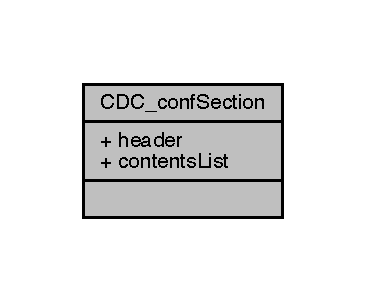
\includegraphics[width=175pt]{struct_c_d_c__conf_section__coll__graph}
\end{center}
\end{figure}
\subsection*{Public Attributes}
\begin{DoxyCompactItemize}
\item 
Q\+String \hyperlink{struct_c_d_c__conf_section_a4cd2f8b187662844e29d66c4ddab046e}{header}
\item 
Q\+String\+List \hyperlink{struct_c_d_c__conf_section_a67a9f966e4b9bb43d54f1640421b6f72}{contents\+List}
\end{DoxyCompactItemize}


\subsection{Detailed Description}
Structure that contains the header and the contents on each section of a configuration file. 



Definition at line 45 of file cdcdefs.\+h.



\subsection{Member Data Documentation}
\hypertarget{struct_c_d_c__conf_section_a67a9f966e4b9bb43d54f1640421b6f72}{\index{C\+D\+C\+\_\+conf\+Section@{C\+D\+C\+\_\+conf\+Section}!contents\+List@{contents\+List}}
\index{contents\+List@{contents\+List}!C\+D\+C\+\_\+conf\+Section@{C\+D\+C\+\_\+conf\+Section}}
\subsubsection[{contents\+List}]{\setlength{\rightskip}{0pt plus 5cm}Q\+String\+List C\+D\+C\+\_\+conf\+Section\+::contents\+List}}\label{struct_c_d_c__conf_section_a67a9f966e4b9bb43d54f1640421b6f72}


Definition at line 47 of file cdcdefs.\+h.

\hypertarget{struct_c_d_c__conf_section_a4cd2f8b187662844e29d66c4ddab046e}{\index{C\+D\+C\+\_\+conf\+Section@{C\+D\+C\+\_\+conf\+Section}!header@{header}}
\index{header@{header}!C\+D\+C\+\_\+conf\+Section@{C\+D\+C\+\_\+conf\+Section}}
\subsubsection[{header}]{\setlength{\rightskip}{0pt plus 5cm}Q\+String C\+D\+C\+\_\+conf\+Section\+::header}}\label{struct_c_d_c__conf_section_a4cd2f8b187662844e29d66c4ddab046e}


Definition at line 46 of file cdcdefs.\+h.



The documentation for this struct was generated from the following file\+:\begin{DoxyCompactItemize}
\item 
/\+Users/martin/\+Workspaces/qt/crossdocs\+\_\+gui/\hyperlink{cdcdefs_8h}{cdcdefs.\+h}\end{DoxyCompactItemize}

\hypertarget{struct_c_d_c__doc_structural_element}{\section{C\+D\+C\+\_\+doc\+Structural\+Element Struct Reference}
\label{struct_c_d_c__doc_structural_element}\index{C\+D\+C\+\_\+doc\+Structural\+Element@{C\+D\+C\+\_\+doc\+Structural\+Element}}
}


Retains data on the structural sections found in a document's content.  




{\ttfamily \#include $<$cdcdefs.\+h$>$}



Collaboration diagram for C\+D\+C\+\_\+doc\+Structural\+Element\+:\nopagebreak
\begin{figure}[H]
\begin{center}
\leavevmode
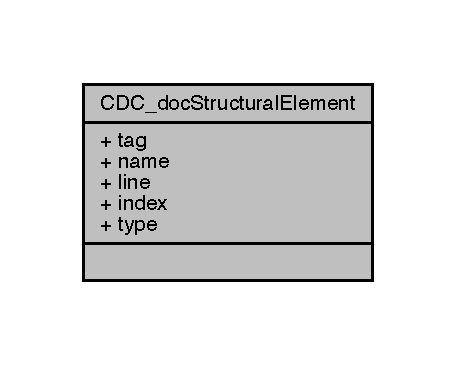
\includegraphics[width=219pt]{struct_c_d_c__doc_structural_element__coll__graph}
\end{center}
\end{figure}
\subsection*{Public Attributes}
\begin{DoxyCompactItemize}
\item 
Q\+String \hyperlink{struct_c_d_c__doc_structural_element_a1c0b32fc629141e98cbbecc122290b5e}{tag}
\item 
Q\+String \hyperlink{struct_c_d_c__doc_structural_element_a03c24ec8c452b6cb8ccf7ea97f8865c8}{name}
\begin{DoxyCompactList}\small\item\em Tag of the structural element (problems will happen if not unique!) \end{DoxyCompactList}\item 
int \hyperlink{struct_c_d_c__doc_structural_element_a115fdf21a90b5c0bc244a8bd395f061d}{line}
\begin{DoxyCompactList}\small\item\em Pretty name of the structural element. \end{DoxyCompactList}\item 
int \hyperlink{struct_c_d_c__doc_structural_element_a009cc844acc8e5d91cc7185ea8a5aab9}{index}
\begin{DoxyCompactList}\small\item\em Line number where the structural element was found. \end{DoxyCompactList}\item 
\hyperlink{cdcdefs_8h_a6116ba1886594c273c61d425c61d6416}{C\+D\+C\+\_\+doc\+Structural\+Element\+Type} \hyperlink{struct_c_d_c__doc_structural_element_a91d8e46c0feb18a294baababa4318f5e}{type}
\begin{DoxyCompactList}\small\item\em Index (column) wherer the structural element. \end{DoxyCompactList}\end{DoxyCompactItemize}


\subsection{Detailed Description}
Retains data on the structural sections found in a document's content. 

Definition at line 89 of file cdcdefs.\+h.



\subsection{Member Data Documentation}
\hypertarget{struct_c_d_c__doc_structural_element_a009cc844acc8e5d91cc7185ea8a5aab9}{\index{C\+D\+C\+\_\+doc\+Structural\+Element@{C\+D\+C\+\_\+doc\+Structural\+Element}!index@{index}}
\index{index@{index}!C\+D\+C\+\_\+doc\+Structural\+Element@{C\+D\+C\+\_\+doc\+Structural\+Element}}
\subsubsection[{index}]{\setlength{\rightskip}{0pt plus 5cm}int C\+D\+C\+\_\+doc\+Structural\+Element\+::index}}\label{struct_c_d_c__doc_structural_element_a009cc844acc8e5d91cc7185ea8a5aab9}


Line number where the structural element was found. 



Definition at line 93 of file cdcdefs.\+h.

\hypertarget{struct_c_d_c__doc_structural_element_a115fdf21a90b5c0bc244a8bd395f061d}{\index{C\+D\+C\+\_\+doc\+Structural\+Element@{C\+D\+C\+\_\+doc\+Structural\+Element}!line@{line}}
\index{line@{line}!C\+D\+C\+\_\+doc\+Structural\+Element@{C\+D\+C\+\_\+doc\+Structural\+Element}}
\subsubsection[{line}]{\setlength{\rightskip}{0pt plus 5cm}int C\+D\+C\+\_\+doc\+Structural\+Element\+::line}}\label{struct_c_d_c__doc_structural_element_a115fdf21a90b5c0bc244a8bd395f061d}


Pretty name of the structural element. 



Definition at line 92 of file cdcdefs.\+h.

\hypertarget{struct_c_d_c__doc_structural_element_a03c24ec8c452b6cb8ccf7ea97f8865c8}{\index{C\+D\+C\+\_\+doc\+Structural\+Element@{C\+D\+C\+\_\+doc\+Structural\+Element}!name@{name}}
\index{name@{name}!C\+D\+C\+\_\+doc\+Structural\+Element@{C\+D\+C\+\_\+doc\+Structural\+Element}}
\subsubsection[{name}]{\setlength{\rightskip}{0pt plus 5cm}Q\+String C\+D\+C\+\_\+doc\+Structural\+Element\+::name}}\label{struct_c_d_c__doc_structural_element_a03c24ec8c452b6cb8ccf7ea97f8865c8}


Tag of the structural element (problems will happen if not unique!) 



Definition at line 91 of file cdcdefs.\+h.

\hypertarget{struct_c_d_c__doc_structural_element_a1c0b32fc629141e98cbbecc122290b5e}{\index{C\+D\+C\+\_\+doc\+Structural\+Element@{C\+D\+C\+\_\+doc\+Structural\+Element}!tag@{tag}}
\index{tag@{tag}!C\+D\+C\+\_\+doc\+Structural\+Element@{C\+D\+C\+\_\+doc\+Structural\+Element}}
\subsubsection[{tag}]{\setlength{\rightskip}{0pt plus 5cm}Q\+String C\+D\+C\+\_\+doc\+Structural\+Element\+::tag}}\label{struct_c_d_c__doc_structural_element_a1c0b32fc629141e98cbbecc122290b5e}


Definition at line 90 of file cdcdefs.\+h.

\hypertarget{struct_c_d_c__doc_structural_element_a91d8e46c0feb18a294baababa4318f5e}{\index{C\+D\+C\+\_\+doc\+Structural\+Element@{C\+D\+C\+\_\+doc\+Structural\+Element}!type@{type}}
\index{type@{type}!C\+D\+C\+\_\+doc\+Structural\+Element@{C\+D\+C\+\_\+doc\+Structural\+Element}}
\subsubsection[{type}]{\setlength{\rightskip}{0pt plus 5cm}{\bf C\+D\+C\+\_\+doc\+Structural\+Element\+Type} C\+D\+C\+\_\+doc\+Structural\+Element\+::type}}\label{struct_c_d_c__doc_structural_element_a91d8e46c0feb18a294baababa4318f5e}


Index (column) wherer the structural element. 



Definition at line 94 of file cdcdefs.\+h.



The documentation for this struct was generated from the following file\+:\begin{DoxyCompactItemize}
\item 
/\+Users/martin/\+Workspaces/qt/crossdocs\+\_\+gui/\hyperlink{cdcdefs_8h}{cdcdefs.\+h}\end{DoxyCompactItemize}

\hypertarget{struct_c_d_c__document}{\section{C\+D\+C\+\_\+document Struct Reference}
\label{struct_c_d_c__document}\index{C\+D\+C\+\_\+document@{C\+D\+C\+\_\+document}}
}


Struct that defines one document's parameters. Each document generates independent.  




{\ttfamily \#include $<$cdcdefs.\+h$>$}



Collaboration diagram for C\+D\+C\+\_\+document\+:\nopagebreak
\begin{figure}[H]
\begin{center}
\leavevmode
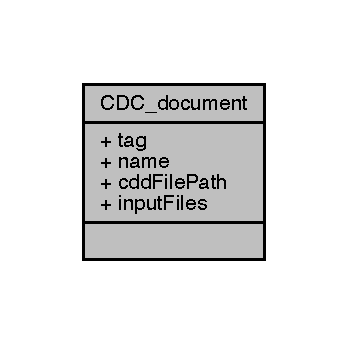
\includegraphics[width=167pt]{struct_c_d_c__document__coll__graph}
\end{center}
\end{figure}
\subsection*{Public Attributes}
\begin{DoxyCompactItemize}
\item 
Q\+String \hyperlink{struct_c_d_c__document_a99da5d8aeec9a1b01a71cb01101aeffd}{tag}
\item 
Q\+String \hyperlink{struct_c_d_c__document_ad2a1ffe07e12dd635b6f0325633c462c}{name}
\begin{DoxyCompactList}\small\item\em Doc tag. Can be used for relative search within a tree if cdd\+File is empty. \end{DoxyCompactList}\item 
Q\+String \hyperlink{struct_c_d_c__document_a6b9d0b788a21919f9abfe32ea84925cb}{cdd\+File\+Path}
\begin{DoxyCompactList}\small\item\em Presentable name. \end{DoxyCompactList}\item 
Q\+List$<$ Q\+File $\ast$ $>$ \hyperlink{struct_c_d_c__document_a22550856ea998c3102deb2b8075d128e}{input\+Files}
\begin{DoxyCompactList}\small\item\em Absolute path for document's cdd configuration file. \end{DoxyCompactList}\end{DoxyCompactItemize}


\subsection{Detailed Description}
Struct that defines one document's parameters. Each document generates independent. 

Definition at line 81 of file cdcdefs.\+h.



\subsection{Member Data Documentation}
\hypertarget{struct_c_d_c__document_a6b9d0b788a21919f9abfe32ea84925cb}{\index{C\+D\+C\+\_\+document@{C\+D\+C\+\_\+document}!cdd\+File\+Path@{cdd\+File\+Path}}
\index{cdd\+File\+Path@{cdd\+File\+Path}!C\+D\+C\+\_\+document@{C\+D\+C\+\_\+document}}
\subsubsection[{cdd\+File\+Path}]{\setlength{\rightskip}{0pt plus 5cm}Q\+String C\+D\+C\+\_\+document\+::cdd\+File\+Path}}\label{struct_c_d_c__document_a6b9d0b788a21919f9abfe32ea84925cb}


Presentable name. 



Definition at line 84 of file cdcdefs.\+h.

\hypertarget{struct_c_d_c__document_a22550856ea998c3102deb2b8075d128e}{\index{C\+D\+C\+\_\+document@{C\+D\+C\+\_\+document}!input\+Files@{input\+Files}}
\index{input\+Files@{input\+Files}!C\+D\+C\+\_\+document@{C\+D\+C\+\_\+document}}
\subsubsection[{input\+Files}]{\setlength{\rightskip}{0pt plus 5cm}Q\+List$<$Q\+File $\ast$$>$ C\+D\+C\+\_\+document\+::input\+Files}}\label{struct_c_d_c__document_a22550856ea998c3102deb2b8075d128e}


Absolute path for document's cdd configuration file. 



Definition at line 85 of file cdcdefs.\+h.

\hypertarget{struct_c_d_c__document_ad2a1ffe07e12dd635b6f0325633c462c}{\index{C\+D\+C\+\_\+document@{C\+D\+C\+\_\+document}!name@{name}}
\index{name@{name}!C\+D\+C\+\_\+document@{C\+D\+C\+\_\+document}}
\subsubsection[{name}]{\setlength{\rightskip}{0pt plus 5cm}Q\+String C\+D\+C\+\_\+document\+::name}}\label{struct_c_d_c__document_ad2a1ffe07e12dd635b6f0325633c462c}


Doc tag. Can be used for relative search within a tree if cdd\+File is empty. 



Definition at line 83 of file cdcdefs.\+h.

\hypertarget{struct_c_d_c__document_a99da5d8aeec9a1b01a71cb01101aeffd}{\index{C\+D\+C\+\_\+document@{C\+D\+C\+\_\+document}!tag@{tag}}
\index{tag@{tag}!C\+D\+C\+\_\+document@{C\+D\+C\+\_\+document}}
\subsubsection[{tag}]{\setlength{\rightskip}{0pt plus 5cm}Q\+String C\+D\+C\+\_\+document\+::tag}}\label{struct_c_d_c__document_a99da5d8aeec9a1b01a71cb01101aeffd}


Definition at line 82 of file cdcdefs.\+h.



The documentation for this struct was generated from the following file\+:\begin{DoxyCompactItemize}
\item 
/\+Users/martin/\+Workspaces/qt/crossdocs\+\_\+gui/\hyperlink{cdcdefs_8h}{cdcdefs.\+h}\end{DoxyCompactItemize}

\hypertarget{structdocument_worker_1_1_c_d_c__input_file}{\section{document\+Worker\+:\+:C\+D\+C\+\_\+input\+File Struct Reference}
\label{structdocument_worker_1_1_c_d_c__input_file}\index{document\+Worker\+::\+C\+D\+C\+\_\+input\+File@{document\+Worker\+::\+C\+D\+C\+\_\+input\+File}}
}


Configuration file for document.  




Collaboration diagram for document\+Worker\+:\+:C\+D\+C\+\_\+input\+File\+:\nopagebreak
\begin{figure}[H]
\begin{center}
\leavevmode
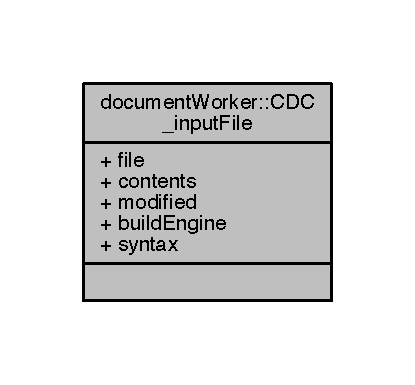
\includegraphics[width=199pt]{structdocument_worker_1_1_c_d_c__input_file__coll__graph}
\end{center}
\end{figure}
\subsection*{Public Attributes}
\begin{DoxyCompactItemize}
\item 
Q\+File $\ast$ \hyperlink{structdocument_worker_1_1_c_d_c__input_file_a807c1fdfcb9e3d0d1112e7fa940505b8}{file}
\item 
Q\+String \hyperlink{structdocument_worker_1_1_c_d_c__input_file_af38edb5a0dfeda3255dd655e736001e0}{contents}
\begin{DoxyCompactList}\small\item\em Stores Q\+File of n-\/th input file. \end{DoxyCompactList}\item 
bool \hyperlink{structdocument_worker_1_1_c_d_c__input_file_a1d8506dc892dc3214443fd12e4c00a95}{modified}
\begin{DoxyCompactList}\small\item\em Stores loaded plain-\/text contents of n-\/th file. \end{DoxyCompactList}\item 
\hyperlink{cdcdefs_8h_abd38cc943467f0d66216a60454d5ee06}{C\+D\+C\+\_\+build\+Engine} \hyperlink{structdocument_worker_1_1_c_d_c__input_file_a31bc229e003dfd135332eb1d57d982f0}{build\+Engine}
\begin{DoxyCompactList}\small\item\em Stores T\+R\+U\+E if file the n-\/th file was modified and not saved. \end{DoxyCompactList}\item 
\hyperlink{cdcdefs_8h_ab649dd84a9663b16384131638df4d313}{C\+D\+C\+\_\+file\+Syntax} \hyperlink{structdocument_worker_1_1_c_d_c__input_file_a7d61569171fa87894c81e9b85575d1be}{syntax}
\begin{DoxyCompactList}\small\item\em Input file's build engine. Defaults to document's setting . \end{DoxyCompactList}\end{DoxyCompactItemize}


\subsection{Detailed Description}
Configuration file for document. 

Definition at line 113 of file documentworker.\+h.



\subsection{Member Data Documentation}
\hypertarget{structdocument_worker_1_1_c_d_c__input_file_a31bc229e003dfd135332eb1d57d982f0}{\index{document\+Worker\+::\+C\+D\+C\+\_\+input\+File@{document\+Worker\+::\+C\+D\+C\+\_\+input\+File}!build\+Engine@{build\+Engine}}
\index{build\+Engine@{build\+Engine}!document\+Worker\+::\+C\+D\+C\+\_\+input\+File@{document\+Worker\+::\+C\+D\+C\+\_\+input\+File}}
\subsubsection[{build\+Engine}]{\setlength{\rightskip}{0pt plus 5cm}{\bf C\+D\+C\+\_\+build\+Engine} document\+Worker\+::\+C\+D\+C\+\_\+input\+File\+::build\+Engine}}\label{structdocument_worker_1_1_c_d_c__input_file_a31bc229e003dfd135332eb1d57d982f0}


Stores T\+R\+U\+E if file the n-\/th file was modified and not saved. 



Definition at line 117 of file documentworker.\+h.

\hypertarget{structdocument_worker_1_1_c_d_c__input_file_af38edb5a0dfeda3255dd655e736001e0}{\index{document\+Worker\+::\+C\+D\+C\+\_\+input\+File@{document\+Worker\+::\+C\+D\+C\+\_\+input\+File}!contents@{contents}}
\index{contents@{contents}!document\+Worker\+::\+C\+D\+C\+\_\+input\+File@{document\+Worker\+::\+C\+D\+C\+\_\+input\+File}}
\subsubsection[{contents}]{\setlength{\rightskip}{0pt plus 5cm}Q\+String document\+Worker\+::\+C\+D\+C\+\_\+input\+File\+::contents}}\label{structdocument_worker_1_1_c_d_c__input_file_af38edb5a0dfeda3255dd655e736001e0}


Stores Q\+File of n-\/th input file. 



Definition at line 115 of file documentworker.\+h.

\hypertarget{structdocument_worker_1_1_c_d_c__input_file_a807c1fdfcb9e3d0d1112e7fa940505b8}{\index{document\+Worker\+::\+C\+D\+C\+\_\+input\+File@{document\+Worker\+::\+C\+D\+C\+\_\+input\+File}!file@{file}}
\index{file@{file}!document\+Worker\+::\+C\+D\+C\+\_\+input\+File@{document\+Worker\+::\+C\+D\+C\+\_\+input\+File}}
\subsubsection[{file}]{\setlength{\rightskip}{0pt plus 5cm}Q\+File$\ast$ document\+Worker\+::\+C\+D\+C\+\_\+input\+File\+::file}}\label{structdocument_worker_1_1_c_d_c__input_file_a807c1fdfcb9e3d0d1112e7fa940505b8}


Definition at line 114 of file documentworker.\+h.

\hypertarget{structdocument_worker_1_1_c_d_c__input_file_a1d8506dc892dc3214443fd12e4c00a95}{\index{document\+Worker\+::\+C\+D\+C\+\_\+input\+File@{document\+Worker\+::\+C\+D\+C\+\_\+input\+File}!modified@{modified}}
\index{modified@{modified}!document\+Worker\+::\+C\+D\+C\+\_\+input\+File@{document\+Worker\+::\+C\+D\+C\+\_\+input\+File}}
\subsubsection[{modified}]{\setlength{\rightskip}{0pt plus 5cm}bool document\+Worker\+::\+C\+D\+C\+\_\+input\+File\+::modified}}\label{structdocument_worker_1_1_c_d_c__input_file_a1d8506dc892dc3214443fd12e4c00a95}


Stores loaded plain-\/text contents of n-\/th file. 



Definition at line 116 of file documentworker.\+h.

\hypertarget{structdocument_worker_1_1_c_d_c__input_file_a7d61569171fa87894c81e9b85575d1be}{\index{document\+Worker\+::\+C\+D\+C\+\_\+input\+File@{document\+Worker\+::\+C\+D\+C\+\_\+input\+File}!syntax@{syntax}}
\index{syntax@{syntax}!document\+Worker\+::\+C\+D\+C\+\_\+input\+File@{document\+Worker\+::\+C\+D\+C\+\_\+input\+File}}
\subsubsection[{syntax}]{\setlength{\rightskip}{0pt plus 5cm}{\bf C\+D\+C\+\_\+file\+Syntax} document\+Worker\+::\+C\+D\+C\+\_\+input\+File\+::syntax}}\label{structdocument_worker_1_1_c_d_c__input_file_a7d61569171fa87894c81e9b85575d1be}


Input file's build engine. Defaults to document's setting . 



Definition at line 118 of file documentworker.\+h.



The documentation for this struct was generated from the following file\+:\begin{DoxyCompactItemize}
\item 
/\+Users/martin/\+Workspaces/qt/crossdocs\+\_\+gui/\hyperlink{documentworker_8h}{documentworker.\+h}\end{DoxyCompactItemize}

\hypertarget{classcdc_main_window}{\section{cdc\+Main\+Window Class Reference}
\label{classcdc_main_window}\index{cdc\+Main\+Window@{cdc\+Main\+Window}}
}


{\ttfamily \#include $<$cdcmainwindow.\+h$>$}



Inheritance diagram for cdc\+Main\+Window\+:\nopagebreak
\begin{figure}[H]
\begin{center}
\leavevmode
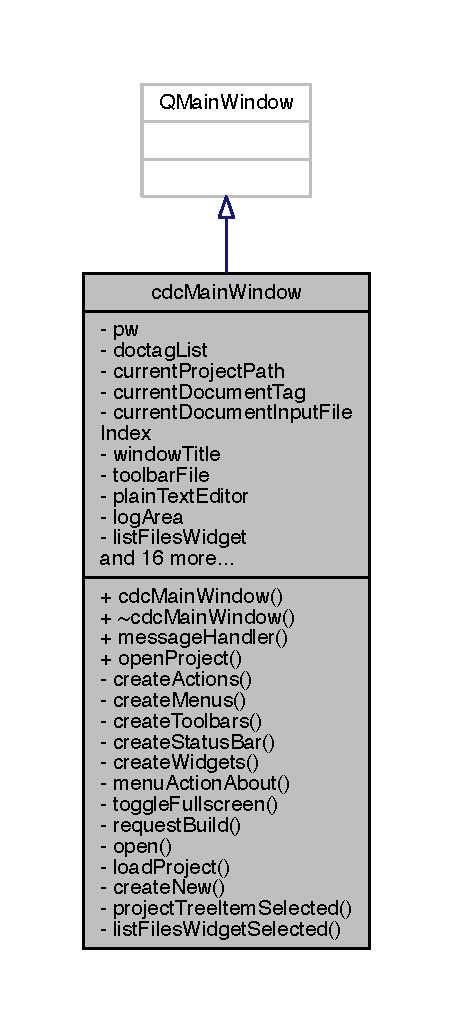
\includegraphics[width=217pt]{classcdc_main_window__inherit__graph}
\end{center}
\end{figure}


Collaboration diagram for cdc\+Main\+Window\+:\nopagebreak
\begin{figure}[H]
\begin{center}
\leavevmode
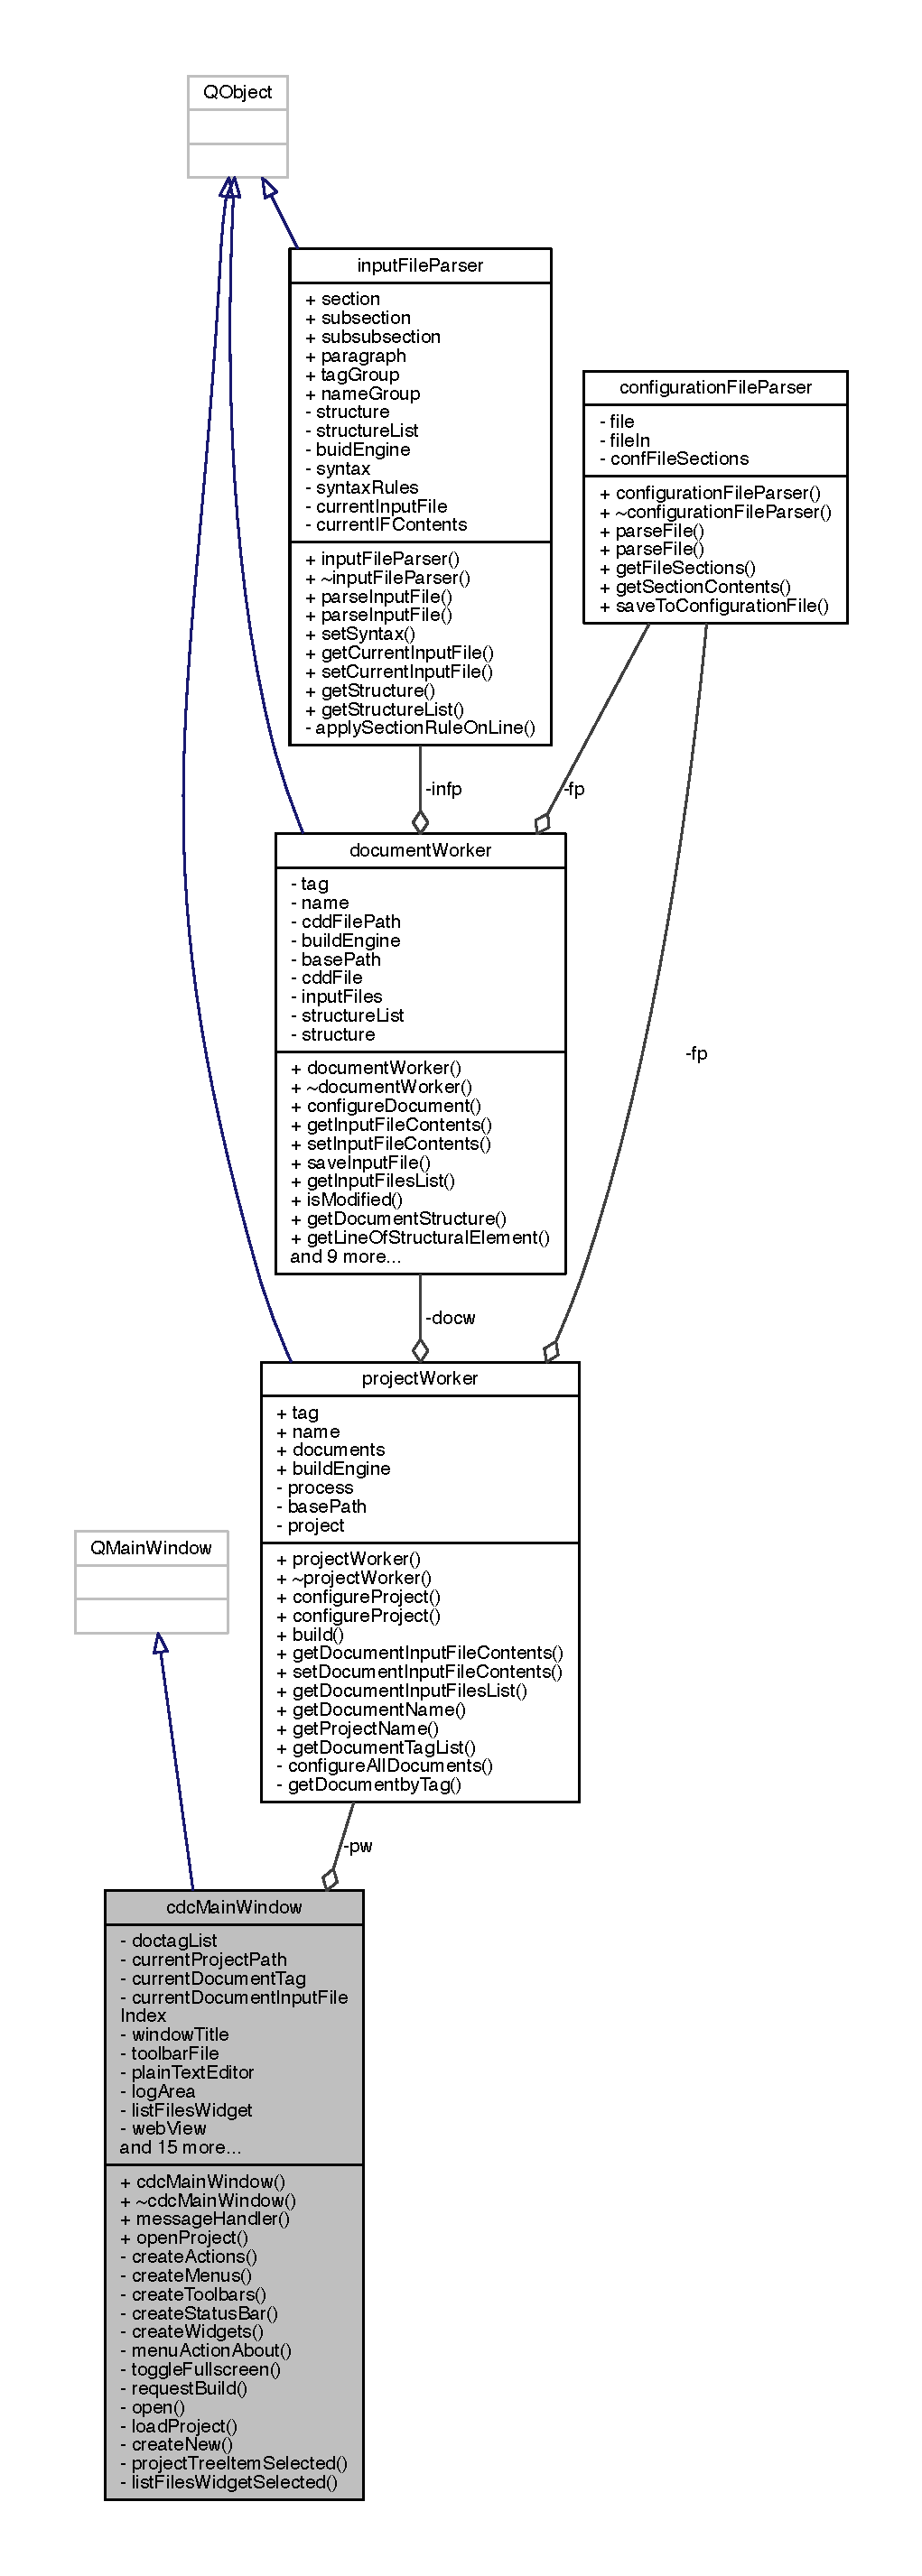
\includegraphics[height=550pt]{classcdc_main_window__coll__graph}
\end{center}
\end{figure}
\subsection*{Public Slots}
\begin{DoxyCompactItemize}
\item 
void \hyperlink{classcdc_main_window_afe66a2955f78dca82931e14113abd139}{message\+Handler} (Qt\+Msg\+Type type, const char $\ast$msg, bool is\+Dialog)
\item 
void \hyperlink{classcdc_main_window_ab0992edf8cb9284fe7068bd24aabce0d}{open\+Project} (Q\+String file\+Name=Q\+String\+::\+Q\+String(\char`\"{}\char`\"{}))
\end{DoxyCompactItemize}
\subsection*{Public Member Functions}
\begin{DoxyCompactItemize}
\item 
\hyperlink{classcdc_main_window_a152934d912eba5b8d46ffc909705e753}{cdc\+Main\+Window} (Q\+Widget $\ast$parent=0)
\item 
\hyperlink{classcdc_main_window_afc27c52a07905eb44b90265ccb716bc4}{$\sim$cdc\+Main\+Window} ()
\end{DoxyCompactItemize}
\subsection*{Private Slots}
\begin{DoxyCompactItemize}
\item 
void \hyperlink{classcdc_main_window_aae83c9e69786db44cddbedc869e778ee}{menu\+Action\+About} ()
\item 
void \hyperlink{classcdc_main_window_a4c5cd1095df7a9c7b81d492f8584cc7c}{toggle\+Fullscreen} (bool)
\item 
void \hyperlink{classcdc_main_window_a3bfb1c19a7c341ec29209ce671a31244}{request\+Build} ()
\item 
void \hyperlink{classcdc_main_window_a788d8721e83a4bdfb7f29364f43c2664}{open} ()
\item 
void \hyperlink{classcdc_main_window_a270552b000c6e8142dfa58d24621b571}{load\+Project} ()
\item 
void \hyperlink{classcdc_main_window_a9922f5b1de24ca399aa8ad18758e9339}{create\+New} ()
\item 
void \hyperlink{classcdc_main_window_ac03dde5c25ceda203773aabb84bc24ef}{project\+Tree\+Item\+Selected} ()
\item 
void \hyperlink{classcdc_main_window_a95ba6457d858d22fc15246a6f1deaf71}{list\+Files\+Widget\+Selected} ()
\end{DoxyCompactItemize}
\subsection*{Private Member Functions}
\begin{DoxyCompactItemize}
\item 
void \hyperlink{classcdc_main_window_a6da58a8decd1c57d5b61a318baff0894}{create\+Actions} ()
\item 
void \hyperlink{classcdc_main_window_ae4951ac1c365e34d3182cca170e1bf9f}{create\+Menus} ()
\item 
void \hyperlink{classcdc_main_window_a1e637d866cb42165fb7f27c92d40f5e0}{create\+Toolbars} ()
\item 
void \hyperlink{classcdc_main_window_a15906e7ebff4d21e4b4e35774458e99e}{create\+Status\+Bar} ()
\item 
void \hyperlink{classcdc_main_window_a14699c304214e6939300e2a9945e9bbe}{create\+Widgets} ()
\end{DoxyCompactItemize}
\subsection*{Private Attributes}
\begin{DoxyCompactItemize}
\item 
\hyperlink{classproject_worker}{project\+Worker} $\ast$ \hyperlink{classcdc_main_window_a2ab9ee82b6b3a303bfecaa9f477f8595}{pw}
\item 
Q\+String\+List \hyperlink{classcdc_main_window_aca67c5aa9dee926f1ea9190b23709d7d}{doctag\+List}
\item 
Q\+String \hyperlink{classcdc_main_window_a2a636f427e14608215f1115de3369ded}{current\+Project\+Path}
\item 
Q\+String \hyperlink{classcdc_main_window_aa819ac3dd6acd06ae65d136a4f683e97}{current\+Document\+Tag}
\item 
int \hyperlink{classcdc_main_window_aca3064de74e5cf938c009d5ab8f2e805}{current\+Document\+Input\+File\+Index}
\item 
Q\+String \hyperlink{classcdc_main_window_a1ca58eeaa25a25ef5f1dbc6772d0853a}{window\+Title}
\item 
Q\+Tool\+Bar $\ast$ \hyperlink{classcdc_main_window_a5d1a9fb552d49501601e0f815e1205f0}{toolbar\+File}
\item 
Q\+Text\+Edit $\ast$ \hyperlink{classcdc_main_window_ad2f451768cf6b6d2d2e828a0598a7b67}{plain\+Text\+Editor}
\item 
Q\+Text\+Edit $\ast$ \hyperlink{classcdc_main_window_acf5379568430403fc8080d3e2fdc22f4}{log\+Area}
\item 
Q\+List\+Widget $\ast$ \hyperlink{classcdc_main_window_a5e658d4cb5bc593d10e30b9fbf680c84}{list\+Files\+Widget}
\item 
Q\+Web\+View $\ast$ \hyperlink{classcdc_main_window_a9b0360abdaa43b49ba788baf4dab83fa}{web\+View}
\item 
Q\+Tree\+View $\ast$ \hyperlink{classcdc_main_window_a5adfe51057f2e53feddc1367cf50609e}{tree\+Project}
\item 
Q\+Menu $\ast$ \hyperlink{classcdc_main_window_a10261cfc57f6d2f7dc8d69c449ded903}{menu\+File}
\item 
Q\+Menu $\ast$ \hyperlink{classcdc_main_window_a0d41f03c46c693ee6a4d82b807aaca6b}{menu\+Edit}
\item 
Q\+Menu $\ast$ \hyperlink{classcdc_main_window_a8ad1d65233c7c537387d633e73693fb2}{menu\+Help}
\item 
Q\+Menu $\ast$ \hyperlink{classcdc_main_window_aff43f7f9a42d9aaa9f468acc48399cc2}{menu\+View}
\item 
Q\+Action $\ast$ \hyperlink{classcdc_main_window_a31bfc3ddbac31b5a2b98871fefd97bee}{action\+Exit}
\item 
Q\+Action $\ast$ \hyperlink{classcdc_main_window_acaec69cb2e1bcea186dbad417d0d354c}{action\+Open}
\item 
Q\+Action $\ast$ \hyperlink{classcdc_main_window_a5b9b87879809858881d876d1108a7900}{action\+Open\+Project}
\item 
Q\+Action $\ast$ \hyperlink{classcdc_main_window_a7e1acb848a40fdf54379bfb5225cf444}{action\+New}
\item 
Q\+Action $\ast$ \hyperlink{classcdc_main_window_a2eda25173588377e053709151eedb45b}{action\+Build}
\item 
Q\+Action $\ast$ \hyperlink{classcdc_main_window_abf4b137386bb0359be919260b3fa191e}{action\+Test}
\item 
Q\+Action $\ast$ \hyperlink{classcdc_main_window_a8a7300a5a0add46d6169ced5671307f9}{action\+About}
\item 
Q\+Action $\ast$ \hyperlink{classcdc_main_window_a5777b81d9c0851fac15e8e29bcba8443}{action\+About\+Qt}
\item 
Q\+Action $\ast$ \hyperlink{classcdc_main_window_a78e4d0015c1666c749ebb982d54f9ce4}{action\+Toggle\+Fullscreen}
\item 
Q\+Action $\ast$ \hyperlink{classcdc_main_window_a5a2cda69acc2d963b38593709d0b191e}{action\+Preferences}
\end{DoxyCompactItemize}


\subsection{Detailed Description}


Definition at line 32 of file cdcmainwindow.\+h.



\subsection{Constructor \& Destructor Documentation}
\hypertarget{classcdc_main_window_a152934d912eba5b8d46ffc909705e753}{\index{cdc\+Main\+Window@{cdc\+Main\+Window}!cdc\+Main\+Window@{cdc\+Main\+Window}}
\index{cdc\+Main\+Window@{cdc\+Main\+Window}!cdc\+Main\+Window@{cdc\+Main\+Window}}
\subsubsection[{cdc\+Main\+Window}]{\setlength{\rightskip}{0pt plus 5cm}cdc\+Main\+Window\+::cdc\+Main\+Window (
\begin{DoxyParamCaption}
\item[{Q\+Widget $\ast$}]{parent = {\ttfamily 0}}
\end{DoxyParamCaption}
)}}\label{classcdc_main_window_a152934d912eba5b8d46ffc909705e753}


Definition at line 24 of file cdcmainwindow.\+cpp.

\hypertarget{classcdc_main_window_afc27c52a07905eb44b90265ccb716bc4}{\index{cdc\+Main\+Window@{cdc\+Main\+Window}!````~cdc\+Main\+Window@{$\sim$cdc\+Main\+Window}}
\index{````~cdc\+Main\+Window@{$\sim$cdc\+Main\+Window}!cdc\+Main\+Window@{cdc\+Main\+Window}}
\subsubsection[{$\sim$cdc\+Main\+Window}]{\setlength{\rightskip}{0pt plus 5cm}cdc\+Main\+Window\+::$\sim$cdc\+Main\+Window (
\begin{DoxyParamCaption}
{}
\end{DoxyParamCaption}
)}}\label{classcdc_main_window_afc27c52a07905eb44b90265ccb716bc4}


Definition at line 44 of file cdcmainwindow.\+cpp.



\subsection{Member Function Documentation}
\hypertarget{classcdc_main_window_a6da58a8decd1c57d5b61a318baff0894}{\index{cdc\+Main\+Window@{cdc\+Main\+Window}!create\+Actions@{create\+Actions}}
\index{create\+Actions@{create\+Actions}!cdc\+Main\+Window@{cdc\+Main\+Window}}
\subsubsection[{create\+Actions}]{\setlength{\rightskip}{0pt plus 5cm}void cdc\+Main\+Window\+::create\+Actions (
\begin{DoxyParamCaption}
{}
\end{DoxyParamCaption}
)\hspace{0.3cm}{\ttfamily [private]}}}\label{classcdc_main_window_a6da58a8decd1c57d5b61a318baff0894}


Definition at line 208 of file cdcmainwindow.\+cpp.

\hypertarget{classcdc_main_window_ae4951ac1c365e34d3182cca170e1bf9f}{\index{cdc\+Main\+Window@{cdc\+Main\+Window}!create\+Menus@{create\+Menus}}
\index{create\+Menus@{create\+Menus}!cdc\+Main\+Window@{cdc\+Main\+Window}}
\subsubsection[{create\+Menus}]{\setlength{\rightskip}{0pt plus 5cm}void cdc\+Main\+Window\+::create\+Menus (
\begin{DoxyParamCaption}
{}
\end{DoxyParamCaption}
)\hspace{0.3cm}{\ttfamily [private]}}}\label{classcdc_main_window_ae4951ac1c365e34d3182cca170e1bf9f}


Definition at line 256 of file cdcmainwindow.\+cpp.

\hypertarget{classcdc_main_window_a9922f5b1de24ca399aa8ad18758e9339}{\index{cdc\+Main\+Window@{cdc\+Main\+Window}!create\+New@{create\+New}}
\index{create\+New@{create\+New}!cdc\+Main\+Window@{cdc\+Main\+Window}}
\subsubsection[{create\+New}]{\setlength{\rightskip}{0pt plus 5cm}void cdc\+Main\+Window\+::create\+New (
\begin{DoxyParamCaption}
{}
\end{DoxyParamCaption}
)\hspace{0.3cm}{\ttfamily [private]}, {\ttfamily [slot]}}}\label{classcdc_main_window_a9922f5b1de24ca399aa8ad18758e9339}


Definition at line 138 of file cdcmainwindow.\+cpp.

\hypertarget{classcdc_main_window_a15906e7ebff4d21e4b4e35774458e99e}{\index{cdc\+Main\+Window@{cdc\+Main\+Window}!create\+Status\+Bar@{create\+Status\+Bar}}
\index{create\+Status\+Bar@{create\+Status\+Bar}!cdc\+Main\+Window@{cdc\+Main\+Window}}
\subsubsection[{create\+Status\+Bar}]{\setlength{\rightskip}{0pt plus 5cm}void cdc\+Main\+Window\+::create\+Status\+Bar (
\begin{DoxyParamCaption}
{}
\end{DoxyParamCaption}
)\hspace{0.3cm}{\ttfamily [private]}}}\label{classcdc_main_window_a15906e7ebff4d21e4b4e35774458e99e}


Definition at line 289 of file cdcmainwindow.\+cpp.

\hypertarget{classcdc_main_window_a1e637d866cb42165fb7f27c92d40f5e0}{\index{cdc\+Main\+Window@{cdc\+Main\+Window}!create\+Toolbars@{create\+Toolbars}}
\index{create\+Toolbars@{create\+Toolbars}!cdc\+Main\+Window@{cdc\+Main\+Window}}
\subsubsection[{create\+Toolbars}]{\setlength{\rightskip}{0pt plus 5cm}void cdc\+Main\+Window\+::create\+Toolbars (
\begin{DoxyParamCaption}
{}
\end{DoxyParamCaption}
)\hspace{0.3cm}{\ttfamily [private]}}}\label{classcdc_main_window_a1e637d866cb42165fb7f27c92d40f5e0}


Definition at line 277 of file cdcmainwindow.\+cpp.

\hypertarget{classcdc_main_window_a14699c304214e6939300e2a9945e9bbe}{\index{cdc\+Main\+Window@{cdc\+Main\+Window}!create\+Widgets@{create\+Widgets}}
\index{create\+Widgets@{create\+Widgets}!cdc\+Main\+Window@{cdc\+Main\+Window}}
\subsubsection[{create\+Widgets}]{\setlength{\rightskip}{0pt plus 5cm}void cdc\+Main\+Window\+::create\+Widgets (
\begin{DoxyParamCaption}
{}
\end{DoxyParamCaption}
)\hspace{0.3cm}{\ttfamily [private]}}}\label{classcdc_main_window_a14699c304214e6939300e2a9945e9bbe}


Definition at line 294 of file cdcmainwindow.\+cpp.

\hypertarget{classcdc_main_window_a95ba6457d858d22fc15246a6f1deaf71}{\index{cdc\+Main\+Window@{cdc\+Main\+Window}!list\+Files\+Widget\+Selected@{list\+Files\+Widget\+Selected}}
\index{list\+Files\+Widget\+Selected@{list\+Files\+Widget\+Selected}!cdc\+Main\+Window@{cdc\+Main\+Window}}
\subsubsection[{list\+Files\+Widget\+Selected}]{\setlength{\rightskip}{0pt plus 5cm}void cdc\+Main\+Window\+::list\+Files\+Widget\+Selected (
\begin{DoxyParamCaption}
{}
\end{DoxyParamCaption}
)\hspace{0.3cm}{\ttfamily [private]}, {\ttfamily [slot]}}}\label{classcdc_main_window_a95ba6457d858d22fc15246a6f1deaf71}


Definition at line 162 of file cdcmainwindow.\+cpp.

\hypertarget{classcdc_main_window_a270552b000c6e8142dfa58d24621b571}{\index{cdc\+Main\+Window@{cdc\+Main\+Window}!load\+Project@{load\+Project}}
\index{load\+Project@{load\+Project}!cdc\+Main\+Window@{cdc\+Main\+Window}}
\subsubsection[{load\+Project}]{\setlength{\rightskip}{0pt plus 5cm}void cdc\+Main\+Window\+::load\+Project (
\begin{DoxyParamCaption}
{}
\end{DoxyParamCaption}
)\hspace{0.3cm}{\ttfamily [private]}, {\ttfamily [slot]}}}\label{classcdc_main_window_a270552b000c6e8142dfa58d24621b571}


Definition at line 115 of file cdcmainwindow.\+cpp.

\hypertarget{classcdc_main_window_aae83c9e69786db44cddbedc869e778ee}{\index{cdc\+Main\+Window@{cdc\+Main\+Window}!menu\+Action\+About@{menu\+Action\+About}}
\index{menu\+Action\+About@{menu\+Action\+About}!cdc\+Main\+Window@{cdc\+Main\+Window}}
\subsubsection[{menu\+Action\+About}]{\setlength{\rightskip}{0pt plus 5cm}void cdc\+Main\+Window\+::menu\+Action\+About (
\begin{DoxyParamCaption}
{}
\end{DoxyParamCaption}
)\hspace{0.3cm}{\ttfamily [private]}, {\ttfamily [slot]}}}\label{classcdc_main_window_aae83c9e69786db44cddbedc869e778ee}


Definition at line 56 of file cdcmainwindow.\+cpp.

\hypertarget{classcdc_main_window_afe66a2955f78dca82931e14113abd139}{\index{cdc\+Main\+Window@{cdc\+Main\+Window}!message\+Handler@{message\+Handler}}
\index{message\+Handler@{message\+Handler}!cdc\+Main\+Window@{cdc\+Main\+Window}}
\subsubsection[{message\+Handler}]{\setlength{\rightskip}{0pt plus 5cm}void cdc\+Main\+Window\+::message\+Handler (
\begin{DoxyParamCaption}
\item[{Qt\+Msg\+Type}]{type, }
\item[{const char $\ast$}]{msg, }
\item[{bool}]{is\+Dialog}
\end{DoxyParamCaption}
)\hspace{0.3cm}{\ttfamily [slot]}}}\label{classcdc_main_window_afe66a2955f78dca82931e14113abd139}


Definition at line 171 of file cdcmainwindow.\+cpp.

\hypertarget{classcdc_main_window_a788d8721e83a4bdfb7f29364f43c2664}{\index{cdc\+Main\+Window@{cdc\+Main\+Window}!open@{open}}
\index{open@{open}!cdc\+Main\+Window@{cdc\+Main\+Window}}
\subsubsection[{open}]{\setlength{\rightskip}{0pt plus 5cm}void cdc\+Main\+Window\+::open (
\begin{DoxyParamCaption}
{}
\end{DoxyParamCaption}
)\hspace{0.3cm}{\ttfamily [private]}, {\ttfamily [slot]}}}\label{classcdc_main_window_a788d8721e83a4bdfb7f29364f43c2664}


Definition at line 81 of file cdcmainwindow.\+cpp.

\hypertarget{classcdc_main_window_ab0992edf8cb9284fe7068bd24aabce0d}{\index{cdc\+Main\+Window@{cdc\+Main\+Window}!open\+Project@{open\+Project}}
\index{open\+Project@{open\+Project}!cdc\+Main\+Window@{cdc\+Main\+Window}}
\subsubsection[{open\+Project}]{\setlength{\rightskip}{0pt plus 5cm}void cdc\+Main\+Window\+::open\+Project (
\begin{DoxyParamCaption}
\item[{Q\+String}]{file\+Name = {\ttfamily QString\+:\+:QString(\char`\"{}\char`\"{})}}
\end{DoxyParamCaption}
)\hspace{0.3cm}{\ttfamily [slot]}}}\label{classcdc_main_window_ab0992edf8cb9284fe7068bd24aabce0d}


Definition at line 102 of file cdcmainwindow.\+cpp.

\hypertarget{classcdc_main_window_ac03dde5c25ceda203773aabb84bc24ef}{\index{cdc\+Main\+Window@{cdc\+Main\+Window}!project\+Tree\+Item\+Selected@{project\+Tree\+Item\+Selected}}
\index{project\+Tree\+Item\+Selected@{project\+Tree\+Item\+Selected}!cdc\+Main\+Window@{cdc\+Main\+Window}}
\subsubsection[{project\+Tree\+Item\+Selected}]{\setlength{\rightskip}{0pt plus 5cm}void cdc\+Main\+Window\+::project\+Tree\+Item\+Selected (
\begin{DoxyParamCaption}
{}
\end{DoxyParamCaption}
)\hspace{0.3cm}{\ttfamily [private]}, {\ttfamily [slot]}}}\label{classcdc_main_window_ac03dde5c25ceda203773aabb84bc24ef}


Definition at line 142 of file cdcmainwindow.\+cpp.

\hypertarget{classcdc_main_window_a3bfb1c19a7c341ec29209ce671a31244}{\index{cdc\+Main\+Window@{cdc\+Main\+Window}!request\+Build@{request\+Build}}
\index{request\+Build@{request\+Build}!cdc\+Main\+Window@{cdc\+Main\+Window}}
\subsubsection[{request\+Build}]{\setlength{\rightskip}{0pt plus 5cm}void cdc\+Main\+Window\+::request\+Build (
\begin{DoxyParamCaption}
{}
\end{DoxyParamCaption}
)\hspace{0.3cm}{\ttfamily [private]}, {\ttfamily [slot]}}}\label{classcdc_main_window_a3bfb1c19a7c341ec29209ce671a31244}


Definition at line 61 of file cdcmainwindow.\+cpp.

\hypertarget{classcdc_main_window_a4c5cd1095df7a9c7b81d492f8584cc7c}{\index{cdc\+Main\+Window@{cdc\+Main\+Window}!toggle\+Fullscreen@{toggle\+Fullscreen}}
\index{toggle\+Fullscreen@{toggle\+Fullscreen}!cdc\+Main\+Window@{cdc\+Main\+Window}}
\subsubsection[{toggle\+Fullscreen}]{\setlength{\rightskip}{0pt plus 5cm}void cdc\+Main\+Window\+::toggle\+Fullscreen (
\begin{DoxyParamCaption}
\item[{bool}]{fs}
\end{DoxyParamCaption}
)\hspace{0.3cm}{\ttfamily [private]}, {\ttfamily [slot]}}}\label{classcdc_main_window_a4c5cd1095df7a9c7b81d492f8584cc7c}


Definition at line 50 of file cdcmainwindow.\+cpp.



\subsection{Member Data Documentation}
\hypertarget{classcdc_main_window_a8a7300a5a0add46d6169ced5671307f9}{\index{cdc\+Main\+Window@{cdc\+Main\+Window}!action\+About@{action\+About}}
\index{action\+About@{action\+About}!cdc\+Main\+Window@{cdc\+Main\+Window}}
\subsubsection[{action\+About}]{\setlength{\rightskip}{0pt plus 5cm}Q\+Action$\ast$ cdc\+Main\+Window\+::action\+About\hspace{0.3cm}{\ttfamily [private]}}}\label{classcdc_main_window_a8a7300a5a0add46d6169ced5671307f9}


Definition at line 92 of file cdcmainwindow.\+h.

\hypertarget{classcdc_main_window_a5777b81d9c0851fac15e8e29bcba8443}{\index{cdc\+Main\+Window@{cdc\+Main\+Window}!action\+About\+Qt@{action\+About\+Qt}}
\index{action\+About\+Qt@{action\+About\+Qt}!cdc\+Main\+Window@{cdc\+Main\+Window}}
\subsubsection[{action\+About\+Qt}]{\setlength{\rightskip}{0pt plus 5cm}Q\+Action$\ast$ cdc\+Main\+Window\+::action\+About\+Qt\hspace{0.3cm}{\ttfamily [private]}}}\label{classcdc_main_window_a5777b81d9c0851fac15e8e29bcba8443}


Definition at line 93 of file cdcmainwindow.\+h.

\hypertarget{classcdc_main_window_a2eda25173588377e053709151eedb45b}{\index{cdc\+Main\+Window@{cdc\+Main\+Window}!action\+Build@{action\+Build}}
\index{action\+Build@{action\+Build}!cdc\+Main\+Window@{cdc\+Main\+Window}}
\subsubsection[{action\+Build}]{\setlength{\rightskip}{0pt plus 5cm}Q\+Action$\ast$ cdc\+Main\+Window\+::action\+Build\hspace{0.3cm}{\ttfamily [private]}}}\label{classcdc_main_window_a2eda25173588377e053709151eedb45b}


Definition at line 90 of file cdcmainwindow.\+h.

\hypertarget{classcdc_main_window_a31bfc3ddbac31b5a2b98871fefd97bee}{\index{cdc\+Main\+Window@{cdc\+Main\+Window}!action\+Exit@{action\+Exit}}
\index{action\+Exit@{action\+Exit}!cdc\+Main\+Window@{cdc\+Main\+Window}}
\subsubsection[{action\+Exit}]{\setlength{\rightskip}{0pt plus 5cm}Q\+Action$\ast$ cdc\+Main\+Window\+::action\+Exit\hspace{0.3cm}{\ttfamily [private]}}}\label{classcdc_main_window_a31bfc3ddbac31b5a2b98871fefd97bee}


Definition at line 86 of file cdcmainwindow.\+h.

\hypertarget{classcdc_main_window_a7e1acb848a40fdf54379bfb5225cf444}{\index{cdc\+Main\+Window@{cdc\+Main\+Window}!action\+New@{action\+New}}
\index{action\+New@{action\+New}!cdc\+Main\+Window@{cdc\+Main\+Window}}
\subsubsection[{action\+New}]{\setlength{\rightskip}{0pt plus 5cm}Q\+Action$\ast$ cdc\+Main\+Window\+::action\+New\hspace{0.3cm}{\ttfamily [private]}}}\label{classcdc_main_window_a7e1acb848a40fdf54379bfb5225cf444}


Definition at line 89 of file cdcmainwindow.\+h.

\hypertarget{classcdc_main_window_acaec69cb2e1bcea186dbad417d0d354c}{\index{cdc\+Main\+Window@{cdc\+Main\+Window}!action\+Open@{action\+Open}}
\index{action\+Open@{action\+Open}!cdc\+Main\+Window@{cdc\+Main\+Window}}
\subsubsection[{action\+Open}]{\setlength{\rightskip}{0pt plus 5cm}Q\+Action$\ast$ cdc\+Main\+Window\+::action\+Open\hspace{0.3cm}{\ttfamily [private]}}}\label{classcdc_main_window_acaec69cb2e1bcea186dbad417d0d354c}


Definition at line 87 of file cdcmainwindow.\+h.

\hypertarget{classcdc_main_window_a5b9b87879809858881d876d1108a7900}{\index{cdc\+Main\+Window@{cdc\+Main\+Window}!action\+Open\+Project@{action\+Open\+Project}}
\index{action\+Open\+Project@{action\+Open\+Project}!cdc\+Main\+Window@{cdc\+Main\+Window}}
\subsubsection[{action\+Open\+Project}]{\setlength{\rightskip}{0pt plus 5cm}Q\+Action$\ast$ cdc\+Main\+Window\+::action\+Open\+Project\hspace{0.3cm}{\ttfamily [private]}}}\label{classcdc_main_window_a5b9b87879809858881d876d1108a7900}


Definition at line 88 of file cdcmainwindow.\+h.

\hypertarget{classcdc_main_window_a5a2cda69acc2d963b38593709d0b191e}{\index{cdc\+Main\+Window@{cdc\+Main\+Window}!action\+Preferences@{action\+Preferences}}
\index{action\+Preferences@{action\+Preferences}!cdc\+Main\+Window@{cdc\+Main\+Window}}
\subsubsection[{action\+Preferences}]{\setlength{\rightskip}{0pt plus 5cm}Q\+Action$\ast$ cdc\+Main\+Window\+::action\+Preferences\hspace{0.3cm}{\ttfamily [private]}}}\label{classcdc_main_window_a5a2cda69acc2d963b38593709d0b191e}


Definition at line 95 of file cdcmainwindow.\+h.

\hypertarget{classcdc_main_window_abf4b137386bb0359be919260b3fa191e}{\index{cdc\+Main\+Window@{cdc\+Main\+Window}!action\+Test@{action\+Test}}
\index{action\+Test@{action\+Test}!cdc\+Main\+Window@{cdc\+Main\+Window}}
\subsubsection[{action\+Test}]{\setlength{\rightskip}{0pt plus 5cm}Q\+Action$\ast$ cdc\+Main\+Window\+::action\+Test\hspace{0.3cm}{\ttfamily [private]}}}\label{classcdc_main_window_abf4b137386bb0359be919260b3fa191e}


Definition at line 91 of file cdcmainwindow.\+h.

\hypertarget{classcdc_main_window_a78e4d0015c1666c749ebb982d54f9ce4}{\index{cdc\+Main\+Window@{cdc\+Main\+Window}!action\+Toggle\+Fullscreen@{action\+Toggle\+Fullscreen}}
\index{action\+Toggle\+Fullscreen@{action\+Toggle\+Fullscreen}!cdc\+Main\+Window@{cdc\+Main\+Window}}
\subsubsection[{action\+Toggle\+Fullscreen}]{\setlength{\rightskip}{0pt plus 5cm}Q\+Action$\ast$ cdc\+Main\+Window\+::action\+Toggle\+Fullscreen\hspace{0.3cm}{\ttfamily [private]}}}\label{classcdc_main_window_a78e4d0015c1666c749ebb982d54f9ce4}


Definition at line 94 of file cdcmainwindow.\+h.

\hypertarget{classcdc_main_window_aca3064de74e5cf938c009d5ab8f2e805}{\index{cdc\+Main\+Window@{cdc\+Main\+Window}!current\+Document\+Input\+File\+Index@{current\+Document\+Input\+File\+Index}}
\index{current\+Document\+Input\+File\+Index@{current\+Document\+Input\+File\+Index}!cdc\+Main\+Window@{cdc\+Main\+Window}}
\subsubsection[{current\+Document\+Input\+File\+Index}]{\setlength{\rightskip}{0pt plus 5cm}int cdc\+Main\+Window\+::current\+Document\+Input\+File\+Index\hspace{0.3cm}{\ttfamily [private]}}}\label{classcdc_main_window_aca3064de74e5cf938c009d5ab8f2e805}


Definition at line 70 of file cdcmainwindow.\+h.

\hypertarget{classcdc_main_window_aa819ac3dd6acd06ae65d136a4f683e97}{\index{cdc\+Main\+Window@{cdc\+Main\+Window}!current\+Document\+Tag@{current\+Document\+Tag}}
\index{current\+Document\+Tag@{current\+Document\+Tag}!cdc\+Main\+Window@{cdc\+Main\+Window}}
\subsubsection[{current\+Document\+Tag}]{\setlength{\rightskip}{0pt plus 5cm}Q\+String cdc\+Main\+Window\+::current\+Document\+Tag\hspace{0.3cm}{\ttfamily [private]}}}\label{classcdc_main_window_aa819ac3dd6acd06ae65d136a4f683e97}


Definition at line 69 of file cdcmainwindow.\+h.

\hypertarget{classcdc_main_window_a2a636f427e14608215f1115de3369ded}{\index{cdc\+Main\+Window@{cdc\+Main\+Window}!current\+Project\+Path@{current\+Project\+Path}}
\index{current\+Project\+Path@{current\+Project\+Path}!cdc\+Main\+Window@{cdc\+Main\+Window}}
\subsubsection[{current\+Project\+Path}]{\setlength{\rightskip}{0pt plus 5cm}Q\+String cdc\+Main\+Window\+::current\+Project\+Path\hspace{0.3cm}{\ttfamily [private]}}}\label{classcdc_main_window_a2a636f427e14608215f1115de3369ded}
\hyperlink{classcdc_main_window}{cdc\+Main\+Window} stores only the documents' tags Relevant implementation information is thus kept hidden. 

Definition at line 68 of file cdcmainwindow.\+h.

\hypertarget{classcdc_main_window_aca67c5aa9dee926f1ea9190b23709d7d}{\index{cdc\+Main\+Window@{cdc\+Main\+Window}!doctag\+List@{doctag\+List}}
\index{doctag\+List@{doctag\+List}!cdc\+Main\+Window@{cdc\+Main\+Window}}
\subsubsection[{doctag\+List}]{\setlength{\rightskip}{0pt plus 5cm}Q\+String\+List cdc\+Main\+Window\+::doctag\+List\hspace{0.3cm}{\ttfamily [private]}}}\label{classcdc_main_window_aca67c5aa9dee926f1ea9190b23709d7d}


Definition at line 65 of file cdcmainwindow.\+h.

\hypertarget{classcdc_main_window_a5e658d4cb5bc593d10e30b9fbf680c84}{\index{cdc\+Main\+Window@{cdc\+Main\+Window}!list\+Files\+Widget@{list\+Files\+Widget}}
\index{list\+Files\+Widget@{list\+Files\+Widget}!cdc\+Main\+Window@{cdc\+Main\+Window}}
\subsubsection[{list\+Files\+Widget}]{\setlength{\rightskip}{0pt plus 5cm}Q\+List\+Widget$\ast$ cdc\+Main\+Window\+::list\+Files\+Widget\hspace{0.3cm}{\ttfamily [private]}}}\label{classcdc_main_window_a5e658d4cb5bc593d10e30b9fbf680c84}


Definition at line 77 of file cdcmainwindow.\+h.

\hypertarget{classcdc_main_window_acf5379568430403fc8080d3e2fdc22f4}{\index{cdc\+Main\+Window@{cdc\+Main\+Window}!log\+Area@{log\+Area}}
\index{log\+Area@{log\+Area}!cdc\+Main\+Window@{cdc\+Main\+Window}}
\subsubsection[{log\+Area}]{\setlength{\rightskip}{0pt plus 5cm}Q\+Text\+Edit$\ast$ cdc\+Main\+Window\+::log\+Area\hspace{0.3cm}{\ttfamily [private]}}}\label{classcdc_main_window_acf5379568430403fc8080d3e2fdc22f4}


Definition at line 76 of file cdcmainwindow.\+h.

\hypertarget{classcdc_main_window_a0d41f03c46c693ee6a4d82b807aaca6b}{\index{cdc\+Main\+Window@{cdc\+Main\+Window}!menu\+Edit@{menu\+Edit}}
\index{menu\+Edit@{menu\+Edit}!cdc\+Main\+Window@{cdc\+Main\+Window}}
\subsubsection[{menu\+Edit}]{\setlength{\rightskip}{0pt plus 5cm}Q\+Menu$\ast$ cdc\+Main\+Window\+::menu\+Edit\hspace{0.3cm}{\ttfamily [private]}}}\label{classcdc_main_window_a0d41f03c46c693ee6a4d82b807aaca6b}


Definition at line 82 of file cdcmainwindow.\+h.

\hypertarget{classcdc_main_window_a10261cfc57f6d2f7dc8d69c449ded903}{\index{cdc\+Main\+Window@{cdc\+Main\+Window}!menu\+File@{menu\+File}}
\index{menu\+File@{menu\+File}!cdc\+Main\+Window@{cdc\+Main\+Window}}
\subsubsection[{menu\+File}]{\setlength{\rightskip}{0pt plus 5cm}Q\+Menu$\ast$ cdc\+Main\+Window\+::menu\+File\hspace{0.3cm}{\ttfamily [private]}}}\label{classcdc_main_window_a10261cfc57f6d2f7dc8d69c449ded903}


Definition at line 81 of file cdcmainwindow.\+h.

\hypertarget{classcdc_main_window_a8ad1d65233c7c537387d633e73693fb2}{\index{cdc\+Main\+Window@{cdc\+Main\+Window}!menu\+Help@{menu\+Help}}
\index{menu\+Help@{menu\+Help}!cdc\+Main\+Window@{cdc\+Main\+Window}}
\subsubsection[{menu\+Help}]{\setlength{\rightskip}{0pt plus 5cm}Q\+Menu$\ast$ cdc\+Main\+Window\+::menu\+Help\hspace{0.3cm}{\ttfamily [private]}}}\label{classcdc_main_window_a8ad1d65233c7c537387d633e73693fb2}


Definition at line 83 of file cdcmainwindow.\+h.

\hypertarget{classcdc_main_window_aff43f7f9a42d9aaa9f468acc48399cc2}{\index{cdc\+Main\+Window@{cdc\+Main\+Window}!menu\+View@{menu\+View}}
\index{menu\+View@{menu\+View}!cdc\+Main\+Window@{cdc\+Main\+Window}}
\subsubsection[{menu\+View}]{\setlength{\rightskip}{0pt plus 5cm}Q\+Menu$\ast$ cdc\+Main\+Window\+::menu\+View\hspace{0.3cm}{\ttfamily [private]}}}\label{classcdc_main_window_aff43f7f9a42d9aaa9f468acc48399cc2}


Definition at line 84 of file cdcmainwindow.\+h.

\hypertarget{classcdc_main_window_ad2f451768cf6b6d2d2e828a0598a7b67}{\index{cdc\+Main\+Window@{cdc\+Main\+Window}!plain\+Text\+Editor@{plain\+Text\+Editor}}
\index{plain\+Text\+Editor@{plain\+Text\+Editor}!cdc\+Main\+Window@{cdc\+Main\+Window}}
\subsubsection[{plain\+Text\+Editor}]{\setlength{\rightskip}{0pt plus 5cm}Q\+Text\+Edit$\ast$ cdc\+Main\+Window\+::plain\+Text\+Editor\hspace{0.3cm}{\ttfamily [private]}}}\label{classcdc_main_window_ad2f451768cf6b6d2d2e828a0598a7b67}


Definition at line 75 of file cdcmainwindow.\+h.

\hypertarget{classcdc_main_window_a2ab9ee82b6b3a303bfecaa9f477f8595}{\index{cdc\+Main\+Window@{cdc\+Main\+Window}!pw@{pw}}
\index{pw@{pw}!cdc\+Main\+Window@{cdc\+Main\+Window}}
\subsubsection[{pw}]{\setlength{\rightskip}{0pt plus 5cm}{\bf project\+Worker}$\ast$ cdc\+Main\+Window\+::pw\hspace{0.3cm}{\ttfamily [private]}}}\label{classcdc_main_window_a2ab9ee82b6b3a303bfecaa9f477f8595}


Definition at line 64 of file cdcmainwindow.\+h.

\hypertarget{classcdc_main_window_a5d1a9fb552d49501601e0f815e1205f0}{\index{cdc\+Main\+Window@{cdc\+Main\+Window}!toolbar\+File@{toolbar\+File}}
\index{toolbar\+File@{toolbar\+File}!cdc\+Main\+Window@{cdc\+Main\+Window}}
\subsubsection[{toolbar\+File}]{\setlength{\rightskip}{0pt plus 5cm}Q\+Tool\+Bar$\ast$ cdc\+Main\+Window\+::toolbar\+File\hspace{0.3cm}{\ttfamily [private]}}}\label{classcdc_main_window_a5d1a9fb552d49501601e0f815e1205f0}


Definition at line 74 of file cdcmainwindow.\+h.

\hypertarget{classcdc_main_window_a5adfe51057f2e53feddc1367cf50609e}{\index{cdc\+Main\+Window@{cdc\+Main\+Window}!tree\+Project@{tree\+Project}}
\index{tree\+Project@{tree\+Project}!cdc\+Main\+Window@{cdc\+Main\+Window}}
\subsubsection[{tree\+Project}]{\setlength{\rightskip}{0pt plus 5cm}Q\+Tree\+View$\ast$ cdc\+Main\+Window\+::tree\+Project\hspace{0.3cm}{\ttfamily [private]}}}\label{classcdc_main_window_a5adfe51057f2e53feddc1367cf50609e}


Definition at line 79 of file cdcmainwindow.\+h.

\hypertarget{classcdc_main_window_a9b0360abdaa43b49ba788baf4dab83fa}{\index{cdc\+Main\+Window@{cdc\+Main\+Window}!web\+View@{web\+View}}
\index{web\+View@{web\+View}!cdc\+Main\+Window@{cdc\+Main\+Window}}
\subsubsection[{web\+View}]{\setlength{\rightskip}{0pt plus 5cm}Q\+Web\+View$\ast$ cdc\+Main\+Window\+::web\+View\hspace{0.3cm}{\ttfamily [private]}}}\label{classcdc_main_window_a9b0360abdaa43b49ba788baf4dab83fa}


Definition at line 78 of file cdcmainwindow.\+h.

\hypertarget{classcdc_main_window_a1ca58eeaa25a25ef5f1dbc6772d0853a}{\index{cdc\+Main\+Window@{cdc\+Main\+Window}!window\+Title@{window\+Title}}
\index{window\+Title@{window\+Title}!cdc\+Main\+Window@{cdc\+Main\+Window}}
\subsubsection[{window\+Title}]{\setlength{\rightskip}{0pt plus 5cm}Q\+String cdc\+Main\+Window\+::window\+Title\hspace{0.3cm}{\ttfamily [private]}}}\label{classcdc_main_window_a1ca58eeaa25a25ef5f1dbc6772d0853a}


Definition at line 73 of file cdcmainwindow.\+h.



The documentation for this class was generated from the following files\+:\begin{DoxyCompactItemize}
\item 
/\+Users/martin/\+Workspaces/qt/crossdocs\+\_\+gui/\hyperlink{cdcmainwindow_8h}{cdcmainwindow.\+h}\item 
/\+Users/martin/\+Workspaces/qt/crossdocs\+\_\+gui/\hyperlink{cdcmainwindow_8cpp}{cdcmainwindow.\+cpp}\end{DoxyCompactItemize}

\hypertarget{classconfiguration_file_parser}{\section{configuration\+File\+Parser Class Reference}
\label{classconfiguration_file_parser}\index{configuration\+File\+Parser@{configuration\+File\+Parser}}
}


{\ttfamily \#include $<$configurationfileparser.\+h$>$}



Collaboration diagram for configuration\+File\+Parser\+:\nopagebreak
\begin{figure}[H]
\begin{center}
\leavevmode
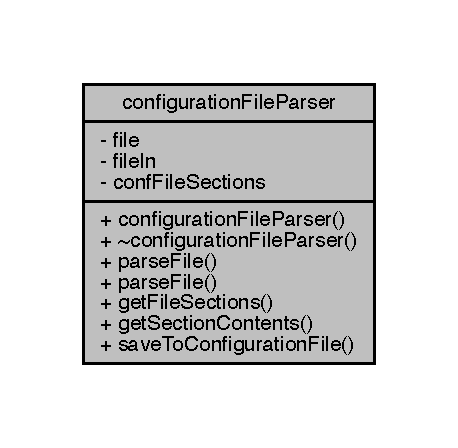
\includegraphics[width=220pt]{classconfiguration_file_parser__coll__graph}
\end{center}
\end{figure}
\subsection*{Public Member Functions}
\begin{DoxyCompactItemize}
\item 
\hyperlink{classconfiguration_file_parser_a88e1b98b7623b2171754db03844b2f2e}{configuration\+File\+Parser} ()
\item 
\hyperlink{classconfiguration_file_parser_ad58b1489837edb4b93a6f9c8ce7c8205}{$\sim$configuration\+File\+Parser} ()
\item 
bool \hyperlink{classconfiguration_file_parser_a54096c6c98ac28b99fcf23da24fcec1d}{parse\+File} (Q\+String fpath, \hyperlink{cdcdefs_8h_a7a1ca742b5a041762c1b5784532bd7fd}{C\+D\+C\+\_\+status} $\ast$ret\+Status=N\+U\+L\+L)
\begin{DoxyCompactList}\small\item\em Parses configuration file in {\itshape fpath}. \end{DoxyCompactList}\item 
bool \hyperlink{classconfiguration_file_parser_aff72b19dd3fb860a9d0917cbb444a504}{parse\+File} (Q\+Dir fpath, \hyperlink{cdcdefs_8h_a7a1ca742b5a041762c1b5784532bd7fd}{C\+D\+C\+\_\+status} $\ast$ret\+Status=N\+U\+L\+L)
\begin{DoxyCompactList}\small\item\em Overloads previous definition of parse\+File to deal with {\itshape Q\+Dir} type of inputs. \end{DoxyCompactList}\item 
Q\+String\+List \hyperlink{classconfiguration_file_parser_a16112cdbdab9ee6ae509aab850697356}{get\+File\+Sections} ()
\begin{DoxyCompactList}\small\item\em Returns the list with all the commands (strings ending with '\+:') found. \end{DoxyCompactList}\item 
Q\+String\+List \hyperlink{classconfiguration_file_parser_a7ca368e0b88cc355f69f572b42763938}{get\+Section\+Contents} (Q\+String sec\+Name)
\begin{DoxyCompactList}\small\item\em Returns the with the contents of a specific section. \end{DoxyCompactList}\item 
bool \hyperlink{classconfiguration_file_parser_ad2e01512b0a5454c0e719982b30699f6}{save\+To\+Configuration\+File} (Q\+String filename, \hyperlink{cdcdefs_8h_adfd872d2c7ac9d9182576c76af28ea98}{C\+D\+C\+\_\+conf\+List} sections)
\begin{DoxyCompactList}\small\item\em Saves {\itshape sections} to {\itshape filename} according to C\+D\+C's syntax. \end{DoxyCompactList}\end{DoxyCompactItemize}
\subsection*{Private Attributes}
\begin{DoxyCompactItemize}
\item 
Q\+File $\ast$ \hyperlink{classconfiguration_file_parser_a699c9d49daf1310225c672e070b93960}{file}
\begin{DoxyCompactList}\small\item\em Current file being handled. \end{DoxyCompactList}\item 
Q\+Text\+Stream $\ast$ \hyperlink{classconfiguration_file_parser_ad85b3428033be9a146b3f35a31b2f756}{file\+In}
\begin{DoxyCompactList}\small\item\em Text stream of the current file handle. \end{DoxyCompactList}\item 
Q\+List$<$ \hyperlink{struct_c_d_c__conf_section}{C\+D\+C\+\_\+conf\+Section} $>$ \hyperlink{classconfiguration_file_parser_a87df99e40e77025aa5a3d9b9f79d7be9}{conf\+File\+Sections}
\begin{DoxyCompactList}\small\item\em List of type \hyperlink{struct_c_d_c__conf_section}{C\+D\+C\+\_\+conf\+Section} containing the sections of the read document. \end{DoxyCompactList}\end{DoxyCompactItemize}


\subsection{Detailed Description}


Definition at line 46 of file configurationfileparser.\+h.



\subsection{Constructor \& Destructor Documentation}
\hypertarget{classconfiguration_file_parser_a88e1b98b7623b2171754db03844b2f2e}{\index{configuration\+File\+Parser@{configuration\+File\+Parser}!configuration\+File\+Parser@{configuration\+File\+Parser}}
\index{configuration\+File\+Parser@{configuration\+File\+Parser}!configuration\+File\+Parser@{configuration\+File\+Parser}}
\subsubsection[{configuration\+File\+Parser}]{\setlength{\rightskip}{0pt plus 5cm}configuration\+File\+Parser\+::configuration\+File\+Parser (
\begin{DoxyParamCaption}
{}
\end{DoxyParamCaption}
)}}\label{classconfiguration_file_parser_a88e1b98b7623b2171754db03844b2f2e}


Definition at line 27 of file configurationfileparser.\+cpp.

\hypertarget{classconfiguration_file_parser_ad58b1489837edb4b93a6f9c8ce7c8205}{\index{configuration\+File\+Parser@{configuration\+File\+Parser}!````~configuration\+File\+Parser@{$\sim$configuration\+File\+Parser}}
\index{````~configuration\+File\+Parser@{$\sim$configuration\+File\+Parser}!configuration\+File\+Parser@{configuration\+File\+Parser}}
\subsubsection[{$\sim$configuration\+File\+Parser}]{\setlength{\rightskip}{0pt plus 5cm}configuration\+File\+Parser\+::$\sim$configuration\+File\+Parser (
\begin{DoxyParamCaption}
{}
\end{DoxyParamCaption}
)}}\label{classconfiguration_file_parser_ad58b1489837edb4b93a6f9c8ce7c8205}


Definition at line 29 of file configurationfileparser.\+cpp.



\subsection{Member Function Documentation}
\hypertarget{classconfiguration_file_parser_a16112cdbdab9ee6ae509aab850697356}{\index{configuration\+File\+Parser@{configuration\+File\+Parser}!get\+File\+Sections@{get\+File\+Sections}}
\index{get\+File\+Sections@{get\+File\+Sections}!configuration\+File\+Parser@{configuration\+File\+Parser}}
\subsubsection[{get\+File\+Sections}]{\setlength{\rightskip}{0pt plus 5cm}Q\+String\+List configuration\+File\+Parser\+::get\+File\+Sections (
\begin{DoxyParamCaption}
{}
\end{DoxyParamCaption}
)}}\label{classconfiguration_file_parser_a16112cdbdab9ee6ae509aab850697356}


Returns the list with all the commands (strings ending with '\+:') found. 



Definition at line 140 of file configurationfileparser.\+cpp.

\hypertarget{classconfiguration_file_parser_a7ca368e0b88cc355f69f572b42763938}{\index{configuration\+File\+Parser@{configuration\+File\+Parser}!get\+Section\+Contents@{get\+Section\+Contents}}
\index{get\+Section\+Contents@{get\+Section\+Contents}!configuration\+File\+Parser@{configuration\+File\+Parser}}
\subsubsection[{get\+Section\+Contents}]{\setlength{\rightskip}{0pt plus 5cm}Q\+String\+List configuration\+File\+Parser\+::get\+Section\+Contents (
\begin{DoxyParamCaption}
\item[{Q\+String}]{sec\+Name}
\end{DoxyParamCaption}
)}}\label{classconfiguration_file_parser_a7ca368e0b88cc355f69f572b42763938}


Returns the with the contents of a specific section. 

Returns an empty list if the section does not exist or has no contents. 

Definition at line 147 of file configurationfileparser.\+cpp.

\hypertarget{classconfiguration_file_parser_a54096c6c98ac28b99fcf23da24fcec1d}{\index{configuration\+File\+Parser@{configuration\+File\+Parser}!parse\+File@{parse\+File}}
\index{parse\+File@{parse\+File}!configuration\+File\+Parser@{configuration\+File\+Parser}}
\subsubsection[{parse\+File}]{\setlength{\rightskip}{0pt plus 5cm}bool configuration\+File\+Parser\+::parse\+File (
\begin{DoxyParamCaption}
\item[{Q\+String}]{fpath, }
\item[{{\bf C\+D\+C\+\_\+status} $\ast$}]{ret\+Status = {\ttfamily NULL}}
\end{DoxyParamCaption}
)}}\label{classconfiguration_file_parser_a54096c6c98ac28b99fcf23da24fcec1d}


Parses configuration file in {\itshape fpath}. 

To implement the read operation of the configuration file in a flexible fashion, a very simple finite state machine is implemented. Four states are possible\+:
\begin{DoxyItemize}
\item {\bfseries idle\+:} Starting state; corresponds to reading an empty line or comment;
\item {\bfseries at-\/header}\+: Found a line with a single string (not whitespace-\/separated) that ends with '\+:'
\item {\bfseries at-\/argument}\+: After finding at least one header (command), found a line with a single string.
\item {\bfseries fail\+:} Something went wrong. Function returns.
\end{DoxyItemize}


\begin{DoxyParams}{Parameters}
{\em fpath} & The full path of the file to be parsed. \\
\hline
\end{DoxyParams}
\begin{DoxyReturn}{Returns}
Whether the file was correctly parsed or not. 
\end{DoxyReturn}
Finite state machine 

Definition at line 33 of file configurationfileparser.\+cpp.

\hypertarget{classconfiguration_file_parser_aff72b19dd3fb860a9d0917cbb444a504}{\index{configuration\+File\+Parser@{configuration\+File\+Parser}!parse\+File@{parse\+File}}
\index{parse\+File@{parse\+File}!configuration\+File\+Parser@{configuration\+File\+Parser}}
\subsubsection[{parse\+File}]{\setlength{\rightskip}{0pt plus 5cm}bool configuration\+File\+Parser\+::parse\+File (
\begin{DoxyParamCaption}
\item[{Q\+Dir}]{fpath, }
\item[{{\bf C\+D\+C\+\_\+status} $\ast$}]{ret\+Status = {\ttfamily NULL}}
\end{DoxyParamCaption}
)\hspace{0.3cm}{\ttfamily [inline]}}}\label{classconfiguration_file_parser_aff72b19dd3fb860a9d0917cbb444a504}


Overloads previous definition of parse\+File to deal with {\itshape Q\+Dir} type of inputs. 



Definition at line 68 of file configurationfileparser.\+h.

\hypertarget{classconfiguration_file_parser_ad2e01512b0a5454c0e719982b30699f6}{\index{configuration\+File\+Parser@{configuration\+File\+Parser}!save\+To\+Configuration\+File@{save\+To\+Configuration\+File}}
\index{save\+To\+Configuration\+File@{save\+To\+Configuration\+File}!configuration\+File\+Parser@{configuration\+File\+Parser}}
\subsubsection[{save\+To\+Configuration\+File}]{\setlength{\rightskip}{0pt plus 5cm}bool configuration\+File\+Parser\+::save\+To\+Configuration\+File (
\begin{DoxyParamCaption}
\item[{Q\+String}]{filename, }
\item[{{\bf C\+D\+C\+\_\+conf\+List}}]{sections}
\end{DoxyParamCaption}
)}}\label{classconfiguration_file_parser_ad2e01512b0a5454c0e719982b30699f6}


Saves {\itshape sections} to {\itshape filename} according to C\+D\+C's syntax. 



Definition at line 158 of file configurationfileparser.\+cpp.



\subsection{Member Data Documentation}
\hypertarget{classconfiguration_file_parser_a87df99e40e77025aa5a3d9b9f79d7be9}{\index{configuration\+File\+Parser@{configuration\+File\+Parser}!conf\+File\+Sections@{conf\+File\+Sections}}
\index{conf\+File\+Sections@{conf\+File\+Sections}!configuration\+File\+Parser@{configuration\+File\+Parser}}
\subsubsection[{conf\+File\+Sections}]{\setlength{\rightskip}{0pt plus 5cm}Q\+List$<${\bf C\+D\+C\+\_\+conf\+Section}$>$ configuration\+File\+Parser\+::conf\+File\+Sections\hspace{0.3cm}{\ttfamily [private]}}}\label{classconfiguration_file_parser_a87df99e40e77025aa5a3d9b9f79d7be9}


List of type \hyperlink{struct_c_d_c__conf_section}{C\+D\+C\+\_\+conf\+Section} containing the sections of the read document. 



Definition at line 93 of file configurationfileparser.\+h.

\hypertarget{classconfiguration_file_parser_a699c9d49daf1310225c672e070b93960}{\index{configuration\+File\+Parser@{configuration\+File\+Parser}!file@{file}}
\index{file@{file}!configuration\+File\+Parser@{configuration\+File\+Parser}}
\subsubsection[{file}]{\setlength{\rightskip}{0pt plus 5cm}Q\+File$\ast$ configuration\+File\+Parser\+::file\hspace{0.3cm}{\ttfamily [private]}}}\label{classconfiguration_file_parser_a699c9d49daf1310225c672e070b93960}


Current file being handled. 



Definition at line 89 of file configurationfileparser.\+h.

\hypertarget{classconfiguration_file_parser_ad85b3428033be9a146b3f35a31b2f756}{\index{configuration\+File\+Parser@{configuration\+File\+Parser}!file\+In@{file\+In}}
\index{file\+In@{file\+In}!configuration\+File\+Parser@{configuration\+File\+Parser}}
\subsubsection[{file\+In}]{\setlength{\rightskip}{0pt plus 5cm}Q\+Text\+Stream$\ast$ configuration\+File\+Parser\+::file\+In\hspace{0.3cm}{\ttfamily [private]}}}\label{classconfiguration_file_parser_ad85b3428033be9a146b3f35a31b2f756}


Text stream of the current file handle. 



Definition at line 91 of file configurationfileparser.\+h.



The documentation for this class was generated from the following files\+:\begin{DoxyCompactItemize}
\item 
/\+Users/martin/\+Workspaces/qt/crossdocs\+\_\+gui/\hyperlink{configurationfileparser_8h}{configurationfileparser.\+h}\item 
/\+Users/martin/\+Workspaces/qt/crossdocs\+\_\+gui/\hyperlink{configurationfileparser_8cpp}{configurationfileparser.\+cpp}\end{DoxyCompactItemize}

\hypertarget{classdocument_worker}{\section{document\+Worker Class Reference}
\label{classdocument_worker}\index{document\+Worker@{document\+Worker}}
}


{\ttfamily \#include $<$documentworker.\+h$>$}



Inheritance diagram for document\+Worker\+:\nopagebreak
\begin{figure}[H]
\begin{center}
\leavevmode
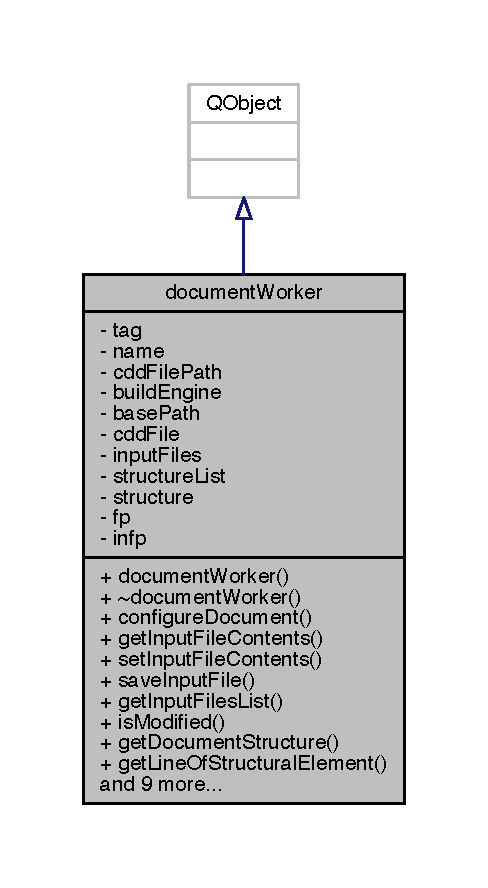
\includegraphics[width=234pt]{classdocument_worker__inherit__graph}
\end{center}
\end{figure}


Collaboration diagram for document\+Worker\+:\nopagebreak
\begin{figure}[H]
\begin{center}
\leavevmode
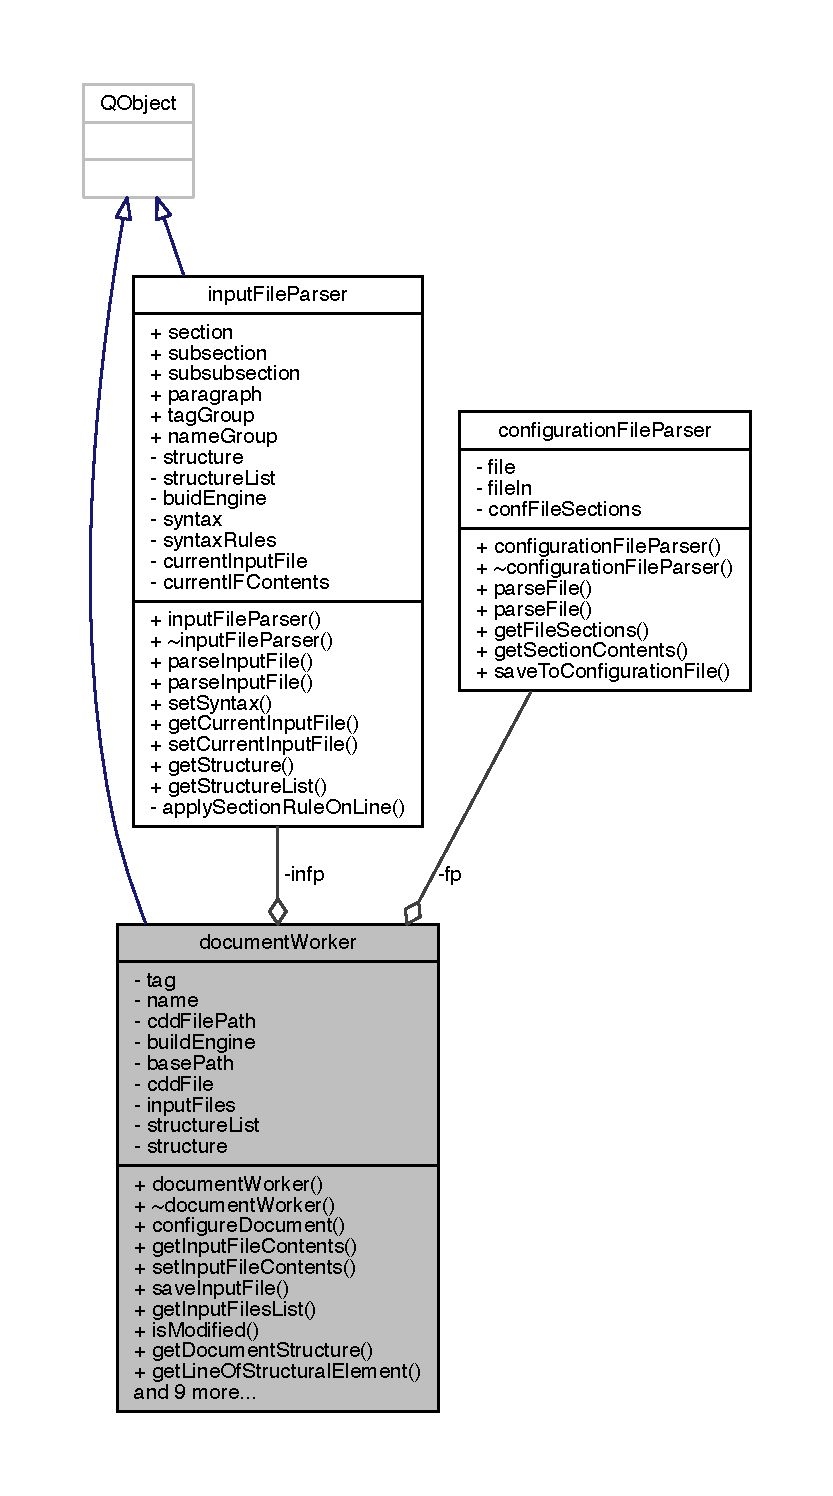
\includegraphics[height=550pt]{classdocument_worker__coll__graph}
\end{center}
\end{figure}
\subsection*{Classes}
\begin{DoxyCompactItemize}
\item 
struct \hyperlink{structdocument_worker_1_1_c_d_c__input_file}{C\+D\+C\+\_\+input\+File}
\begin{DoxyCompactList}\small\item\em Configuration file for document. \end{DoxyCompactList}\end{DoxyCompactItemize}
\subsection*{Public Member Functions}
\begin{DoxyCompactItemize}
\item 
\hyperlink{classdocument_worker_adaab16ea74637a4ebab8eff342aca101}{document\+Worker} (Q\+Object $\ast$parent=0)
\item 
\hyperlink{classdocument_worker_ae51bc4a6da3cd1e769a3690771a4596a}{$\sim$document\+Worker} ()
\item 
bool \hyperlink{classdocument_worker_ab222bea1a23276a9edcce412bf4d524a}{configure\+Document} (Q\+String doc\+Conf\+Path=Q\+String\+::\+Q\+String(\char`\"{}\char`\"{}), \hyperlink{cdcdefs_8h_a7a1ca742b5a041762c1b5784532bd7fd}{C\+D\+C\+\_\+status} $\ast$ret\+Status=N\+U\+L\+L)
\item 
Q\+String \hyperlink{classdocument_worker_aefcc1bfe56d564865818ded4b258c20e}{get\+Input\+File\+Contents} (int index, \hyperlink{cdcdefs_8h_a7a1ca742b5a041762c1b5784532bd7fd}{C\+D\+C\+\_\+status} $\ast$ret\+Status=N\+U\+L\+L)
\begin{DoxyCompactList}\small\item\em Reads contents of file into input\+File\+Contents and the returns them. Reads the file once from the filesystem into application, then return the struct. \end{DoxyCompactList}\item 
void \hyperlink{classdocument_worker_a255b9a45fb833eb41b37461928bf5c4e}{set\+Input\+File\+Contents} (int index, Q\+String content, \hyperlink{cdcdefs_8h_a7a1ca742b5a041762c1b5784532bd7fd}{C\+D\+C\+\_\+status} $\ast$ret\+Status=N\+U\+L\+L)
\begin{DoxyCompactList}\small\item\em Sets the n-\/th input\+File\+Contents element to the given {\itshape content} argument. The contents of the n-\/th input file are altered and the n-\/th {\itshape modified} flag is set. \end{DoxyCompactList}\item 
bool \hyperlink{classdocument_worker_a58ac3a2179ce52dde55b19cf458a7aae}{save\+Input\+File} (int index, \hyperlink{cdcdefs_8h_a7a1ca742b5a041762c1b5784532bd7fd}{C\+D\+C\+\_\+status} $\ast$ret\+Status=N\+U\+L\+L)
\begin{DoxyCompactList}\small\item\em Saves the content of the n-\/th input\+File\+Contents to the file. \end{DoxyCompactList}\item 
Q\+String\+List \hyperlink{classdocument_worker_a827ee0e7099be86c5d20c2fe2fbbafe7}{get\+Input\+Files\+List} ()
\begin{DoxyCompactList}\small\item\em Returns a string list containing the names of all input files. \end{DoxyCompactList}\item 
bool \hyperlink{classdocument_worker_a3549424368574c196404d135eb454a21}{is\+Modified} (int index)
\begin{DoxyCompactList}\small\item\em is\+Modified \end{DoxyCompactList}\item 
Q\+Standard\+Item\+Model $\ast$ \hyperlink{classdocument_worker_a46683d81223a5d0fff3606338e15af9d}{get\+Document\+Structure} ()
\begin{DoxyCompactList}\small\item\em Creates and returns the document's structure (sections, subsections, etc.) Uses the \hyperlink{classinput_file_parser_ad632f2b78c34b72cbaf8105b8762cf9f}{input\+File\+Parser\+::parse\+Input\+File()} method to generate the structure for each input file. Applies this sequentially to each input file and then stitches those structures together, which generates the structure of the \char`\"{}bigger picture\char`\"{}. Simultaneously updates the internal structural element list, that is later used for line number and index information checking. \end{DoxyCompactList}\item 
int \hyperlink{classdocument_worker_a480cf18ca31e3275cb2ea99a1e5b838d}{get\+Line\+Of\+Structural\+Element} (Q\+String elemtag)
\item 
int \hyperlink{classdocument_worker_ac793de2aa348e0d86fb14fa7b14e2f83}{get\+Index\+Of\+Structural\+Element} (Q\+String elemtag)
\item 
Q\+String \hyperlink{classdocument_worker_a9d582a2b8ebb32779ac0b63f3328761a}{get\+Tag} ()
\item 
void \hyperlink{classdocument_worker_ac405fdf4aef95008f2ab00db978017ed}{set\+Tag} (Q\+String value)
\item 
Q\+String \hyperlink{classdocument_worker_abd073cc857adc0df597e6db51449f132}{get\+Name} ()
\item 
void \hyperlink{classdocument_worker_a5b8cf60dd7735536ff94323bebb539f4}{set\+Name} (Q\+String value)
\item 
Q\+String \hyperlink{classdocument_worker_a7c63b5e0013522cc3cac9c347b8a95a5}{get\+Conf\+File\+Path} ()
\item 
void \hyperlink{classdocument_worker_a46f83322e76b85ebc067d48b7b00d5d6}{set\+Conf\+File\+Path} (Q\+String value)
\item 
\hyperlink{cdcdefs_8h_abd38cc943467f0d66216a60454d5ee06}{C\+D\+C\+\_\+build\+Engine} \hyperlink{classdocument_worker_aa33dbe64a646425038a1c80984ba7e17}{get\+Build\+Engine} ()
\item 
void \hyperlink{classdocument_worker_aea01eceaa4dfee75a4ef827a0e300558}{set\+Build\+Engine} (\hyperlink{cdcdefs_8h_abd38cc943467f0d66216a60454d5ee06}{C\+D\+C\+\_\+build\+Engine} value)
\end{DoxyCompactItemize}
\subsection*{Private Attributes}
\begin{DoxyCompactItemize}
\item 
Q\+String \hyperlink{classdocument_worker_a06432e8a28e33071cbb02d7739558ab0}{tag}
\item 
Q\+String \hyperlink{classdocument_worker_af67a64425e1e24d88333afda12eb4d1d}{name}
\item 
Q\+String \hyperlink{classdocument_worker_ad2f131c1430b72e3eab8b5cc9a6e920e}{cdd\+File\+Path}
\item 
\hyperlink{cdcdefs_8h_abd38cc943467f0d66216a60454d5ee06}{C\+D\+C\+\_\+build\+Engine} \hyperlink{classdocument_worker_ab5c27d8e6fd6d96d881d84259dc3538a}{build\+Engine}
\item 
Q\+String \hyperlink{classdocument_worker_a7e7c868c0d0132c45e240eb5e08bbf09}{base\+Path}
\item 
Q\+File $\ast$ \hyperlink{classdocument_worker_ae5dabdc7bbf00675b9a2ed4541e43d63}{cdd\+File}
\begin{DoxyCompactList}\small\item\em Relative to the cdd file. \end{DoxyCompactList}\item 
Q\+List$<$ \hyperlink{structdocument_worker_1_1_c_d_c__input_file}{C\+D\+C\+\_\+input\+File} $>$ \hyperlink{classdocument_worker_a5812c9d02689c044852beb5904c24e82}{input\+Files}
\item 
Q\+List$<$ \hyperlink{struct_c_d_c__doc_structural_element}{C\+D\+C\+\_\+doc\+Structural\+Element} $>$ \hyperlink{classdocument_worker_a18623c1f7f73e476f7c82a02e9752469}{structure\+List}
\item 
Q\+Standard\+Item\+Model $\ast$ \hyperlink{classdocument_worker_af05a07271fc523897d0154400f6dddb0}{structure}
\item 
\hyperlink{classconfiguration_file_parser}{configuration\+File\+Parser} $\ast$ \hyperlink{classdocument_worker_a1825443dff2970960623c0b1979ce85f}{fp}
\item 
\hyperlink{classinput_file_parser}{input\+File\+Parser} $\ast$ \hyperlink{classdocument_worker_a0568a560290f197dcb16ebdb15593e3b}{infp}
\end{DoxyCompactItemize}


\subsection{Detailed Description}


Definition at line 33 of file documentworker.\+h.



\subsection{Constructor \& Destructor Documentation}
\hypertarget{classdocument_worker_adaab16ea74637a4ebab8eff342aca101}{\index{document\+Worker@{document\+Worker}!document\+Worker@{document\+Worker}}
\index{document\+Worker@{document\+Worker}!document\+Worker@{document\+Worker}}
\subsubsection[{document\+Worker}]{\setlength{\rightskip}{0pt plus 5cm}document\+Worker\+::document\+Worker (
\begin{DoxyParamCaption}
\item[{Q\+Object $\ast$}]{parent = {\ttfamily 0}}
\end{DoxyParamCaption}
)}}\label{classdocument_worker_adaab16ea74637a4ebab8eff342aca101}


Definition at line 29 of file documentworker.\+cpp.

\hypertarget{classdocument_worker_ae51bc4a6da3cd1e769a3690771a4596a}{\index{document\+Worker@{document\+Worker}!````~document\+Worker@{$\sim$document\+Worker}}
\index{````~document\+Worker@{$\sim$document\+Worker}!document\+Worker@{document\+Worker}}
\subsubsection[{$\sim$document\+Worker}]{\setlength{\rightskip}{0pt plus 5cm}document\+Worker\+::$\sim$document\+Worker (
\begin{DoxyParamCaption}
{}
\end{DoxyParamCaption}
)}}\label{classdocument_worker_ae51bc4a6da3cd1e769a3690771a4596a}


Definition at line 38 of file documentworker.\+cpp.



\subsection{Member Function Documentation}
\hypertarget{classdocument_worker_ab222bea1a23276a9edcce412bf4d524a}{\index{document\+Worker@{document\+Worker}!configure\+Document@{configure\+Document}}
\index{configure\+Document@{configure\+Document}!document\+Worker@{document\+Worker}}
\subsubsection[{configure\+Document}]{\setlength{\rightskip}{0pt plus 5cm}bool document\+Worker\+::configure\+Document (
\begin{DoxyParamCaption}
\item[{Q\+String}]{doc\+Conf\+Path = {\ttfamily QString\+:\+:QString(\char`\"{}\char`\"{})}, }
\item[{{\bf C\+D\+C\+\_\+status} $\ast$}]{ret\+Status = {\ttfamily NULL}}
\end{DoxyParamCaption}
)}}\label{classdocument_worker_ab222bea1a23276a9edcce412bf4d524a}


Definition at line 49 of file documentworker.\+cpp.

\hypertarget{classdocument_worker_aa33dbe64a646425038a1c80984ba7e17}{\index{document\+Worker@{document\+Worker}!get\+Build\+Engine@{get\+Build\+Engine}}
\index{get\+Build\+Engine@{get\+Build\+Engine}!document\+Worker@{document\+Worker}}
\subsubsection[{get\+Build\+Engine}]{\setlength{\rightskip}{0pt plus 5cm}{\bf C\+D\+C\+\_\+build\+Engine} document\+Worker\+::get\+Build\+Engine (
\begin{DoxyParamCaption}
{}
\end{DoxyParamCaption}
)\hspace{0.3cm}{\ttfamily [inline]}}}\label{classdocument_worker_aa33dbe64a646425038a1c80984ba7e17}


Definition at line 101 of file documentworker.\+h.

\hypertarget{classdocument_worker_a7c63b5e0013522cc3cac9c347b8a95a5}{\index{document\+Worker@{document\+Worker}!get\+Conf\+File\+Path@{get\+Conf\+File\+Path}}
\index{get\+Conf\+File\+Path@{get\+Conf\+File\+Path}!document\+Worker@{document\+Worker}}
\subsubsection[{get\+Conf\+File\+Path}]{\setlength{\rightskip}{0pt plus 5cm}Q\+String document\+Worker\+::get\+Conf\+File\+Path (
\begin{DoxyParamCaption}
{}
\end{DoxyParamCaption}
)\hspace{0.3cm}{\ttfamily [inline]}}}\label{classdocument_worker_a7c63b5e0013522cc3cac9c347b8a95a5}


Definition at line 99 of file documentworker.\+h.

\hypertarget{classdocument_worker_a46683d81223a5d0fff3606338e15af9d}{\index{document\+Worker@{document\+Worker}!get\+Document\+Structure@{get\+Document\+Structure}}
\index{get\+Document\+Structure@{get\+Document\+Structure}!document\+Worker@{document\+Worker}}
\subsubsection[{get\+Document\+Structure}]{\setlength{\rightskip}{0pt plus 5cm}Q\+Standard\+Item\+Model $\ast$ document\+Worker\+::get\+Document\+Structure (
\begin{DoxyParamCaption}
{}
\end{DoxyParamCaption}
)}}\label{classdocument_worker_a46683d81223a5d0fff3606338e15af9d}


Creates and returns the document's structure (sections, subsections, etc.) Uses the \hyperlink{classinput_file_parser_ad632f2b78c34b72cbaf8105b8762cf9f}{input\+File\+Parser\+::parse\+Input\+File()} method to generate the structure for each input file. Applies this sequentially to each input file and then stitches those structures together, which generates the structure of the \char`\"{}bigger picture\char`\"{}. Simultaneously updates the internal structural element list, that is later used for line number and index information checking. 

\begin{DoxyAttention}{Attention}
This whole thing is based on the idea that A\+L\+L stuctural tags in a document are different. Violating this will generate unexpected behaviors! 
\end{DoxyAttention}
\begin{DoxyReturn}{Returns}
The {\bfseries Q\+Standard\+Item\+Model} object containing the representation of the document's structure. 
\end{DoxyReturn}


Definition at line 208 of file documentworker.\+cpp.

\hypertarget{classdocument_worker_ac793de2aa348e0d86fb14fa7b14e2f83}{\index{document\+Worker@{document\+Worker}!get\+Index\+Of\+Structural\+Element@{get\+Index\+Of\+Structural\+Element}}
\index{get\+Index\+Of\+Structural\+Element@{get\+Index\+Of\+Structural\+Element}!document\+Worker@{document\+Worker}}
\subsubsection[{get\+Index\+Of\+Structural\+Element}]{\setlength{\rightskip}{0pt plus 5cm}int document\+Worker\+::get\+Index\+Of\+Structural\+Element (
\begin{DoxyParamCaption}
\item[{Q\+String}]{elemtag}
\end{DoxyParamCaption}
)}}\label{classdocument_worker_ac793de2aa348e0d86fb14fa7b14e2f83}


Definition at line 233 of file documentworker.\+cpp.

\hypertarget{classdocument_worker_aefcc1bfe56d564865818ded4b258c20e}{\index{document\+Worker@{document\+Worker}!get\+Input\+File\+Contents@{get\+Input\+File\+Contents}}
\index{get\+Input\+File\+Contents@{get\+Input\+File\+Contents}!document\+Worker@{document\+Worker}}
\subsubsection[{get\+Input\+File\+Contents}]{\setlength{\rightskip}{0pt plus 5cm}Q\+String document\+Worker\+::get\+Input\+File\+Contents (
\begin{DoxyParamCaption}
\item[{int}]{index, }
\item[{{\bf C\+D\+C\+\_\+status} $\ast$}]{ret\+Status = {\ttfamily NULL}}
\end{DoxyParamCaption}
)}}\label{classdocument_worker_aefcc1bfe56d564865818ded4b258c20e}


Reads contents of file into input\+File\+Contents and the returns them. Reads the file once from the filesystem into application, then return the struct. 


\begin{DoxyParams}{Parameters}
{\em index} & Index of the file in the internal input\+Files structure. \\
\hline
\end{DoxyParams}
\begin{DoxyReturn}{Returns}
String containing the whole plain-\/text file. 
\end{DoxyReturn}


Definition at line 139 of file documentworker.\+cpp.

\hypertarget{classdocument_worker_a827ee0e7099be86c5d20c2fe2fbbafe7}{\index{document\+Worker@{document\+Worker}!get\+Input\+Files\+List@{get\+Input\+Files\+List}}
\index{get\+Input\+Files\+List@{get\+Input\+Files\+List}!document\+Worker@{document\+Worker}}
\subsubsection[{get\+Input\+Files\+List}]{\setlength{\rightskip}{0pt plus 5cm}Q\+String\+List document\+Worker\+::get\+Input\+Files\+List (
\begin{DoxyParamCaption}
{}
\end{DoxyParamCaption}
)}}\label{classdocument_worker_a827ee0e7099be86c5d20c2fe2fbbafe7}


Returns a string list containing the names of all input files. 

\begin{DoxyReturn}{Returns}
Q\+String\+List with full paths of all input files. Empty list if smth went wrong. 
\end{DoxyReturn}


Definition at line 193 of file documentworker.\+cpp.

\hypertarget{classdocument_worker_a480cf18ca31e3275cb2ea99a1e5b838d}{\index{document\+Worker@{document\+Worker}!get\+Line\+Of\+Structural\+Element@{get\+Line\+Of\+Structural\+Element}}
\index{get\+Line\+Of\+Structural\+Element@{get\+Line\+Of\+Structural\+Element}!document\+Worker@{document\+Worker}}
\subsubsection[{get\+Line\+Of\+Structural\+Element}]{\setlength{\rightskip}{0pt plus 5cm}int document\+Worker\+::get\+Line\+Of\+Structural\+Element (
\begin{DoxyParamCaption}
\item[{Q\+String}]{elemtag}
\end{DoxyParamCaption}
)}}\label{classdocument_worker_a480cf18ca31e3275cb2ea99a1e5b838d}


Definition at line 224 of file documentworker.\+cpp.

\hypertarget{classdocument_worker_abd073cc857adc0df597e6db51449f132}{\index{document\+Worker@{document\+Worker}!get\+Name@{get\+Name}}
\index{get\+Name@{get\+Name}!document\+Worker@{document\+Worker}}
\subsubsection[{get\+Name}]{\setlength{\rightskip}{0pt plus 5cm}Q\+String document\+Worker\+::get\+Name (
\begin{DoxyParamCaption}
{}
\end{DoxyParamCaption}
)\hspace{0.3cm}{\ttfamily [inline]}}}\label{classdocument_worker_abd073cc857adc0df597e6db51449f132}


Definition at line 97 of file documentworker.\+h.

\hypertarget{classdocument_worker_a9d582a2b8ebb32779ac0b63f3328761a}{\index{document\+Worker@{document\+Worker}!get\+Tag@{get\+Tag}}
\index{get\+Tag@{get\+Tag}!document\+Worker@{document\+Worker}}
\subsubsection[{get\+Tag}]{\setlength{\rightskip}{0pt plus 5cm}Q\+String document\+Worker\+::get\+Tag (
\begin{DoxyParamCaption}
{}
\end{DoxyParamCaption}
)\hspace{0.3cm}{\ttfamily [inline]}}}\label{classdocument_worker_a9d582a2b8ebb32779ac0b63f3328761a}


Definition at line 95 of file documentworker.\+h.

\hypertarget{classdocument_worker_a3549424368574c196404d135eb454a21}{\index{document\+Worker@{document\+Worker}!is\+Modified@{is\+Modified}}
\index{is\+Modified@{is\+Modified}!document\+Worker@{document\+Worker}}
\subsubsection[{is\+Modified}]{\setlength{\rightskip}{0pt plus 5cm}bool document\+Worker\+::is\+Modified (
\begin{DoxyParamCaption}
\item[{int}]{index}
\end{DoxyParamCaption}
)}}\label{classdocument_worker_a3549424368574c196404d135eb454a21}


is\+Modified 


\begin{DoxyParams}{Parameters}
{\em index} & \\
\hline
\end{DoxyParams}
\begin{DoxyReturn}{Returns}
T\+R\+U\+E if the file at $<$index$>$ was modified through \hyperlink{classdocument_worker_a255b9a45fb833eb41b37461928bf5c4e}{set\+Input\+File\+Contents()} . 
\end{DoxyReturn}


Definition at line 200 of file documentworker.\+cpp.

\hypertarget{classdocument_worker_a58ac3a2179ce52dde55b19cf458a7aae}{\index{document\+Worker@{document\+Worker}!save\+Input\+File@{save\+Input\+File}}
\index{save\+Input\+File@{save\+Input\+File}!document\+Worker@{document\+Worker}}
\subsubsection[{save\+Input\+File}]{\setlength{\rightskip}{0pt plus 5cm}bool document\+Worker\+::save\+Input\+File (
\begin{DoxyParamCaption}
\item[{int}]{index, }
\item[{{\bf C\+D\+C\+\_\+status} $\ast$}]{ret\+Status = {\ttfamily NULL}}
\end{DoxyParamCaption}
)}}\label{classdocument_worker_a58ac3a2179ce52dde55b19cf458a7aae}


Saves the content of the n-\/th input\+File\+Contents to the file. 


\begin{DoxyParams}{Parameters}
{\em index} & Index of the file to be saved. \\
\hline
{\em ret\+Status} & Status of the operation. \\
\hline
\end{DoxyParams}
\begin{DoxyReturn}{Returns}
Whether the operation succeded. 
\end{DoxyReturn}


Definition at line 173 of file documentworker.\+cpp.

\hypertarget{classdocument_worker_aea01eceaa4dfee75a4ef827a0e300558}{\index{document\+Worker@{document\+Worker}!set\+Build\+Engine@{set\+Build\+Engine}}
\index{set\+Build\+Engine@{set\+Build\+Engine}!document\+Worker@{document\+Worker}}
\subsubsection[{set\+Build\+Engine}]{\setlength{\rightskip}{0pt plus 5cm}void document\+Worker\+::set\+Build\+Engine (
\begin{DoxyParamCaption}
\item[{{\bf C\+D\+C\+\_\+build\+Engine}}]{value}
\end{DoxyParamCaption}
)\hspace{0.3cm}{\ttfamily [inline]}}}\label{classdocument_worker_aea01eceaa4dfee75a4ef827a0e300558}


Definition at line 102 of file documentworker.\+h.

\hypertarget{classdocument_worker_a46f83322e76b85ebc067d48b7b00d5d6}{\index{document\+Worker@{document\+Worker}!set\+Conf\+File\+Path@{set\+Conf\+File\+Path}}
\index{set\+Conf\+File\+Path@{set\+Conf\+File\+Path}!document\+Worker@{document\+Worker}}
\subsubsection[{set\+Conf\+File\+Path}]{\setlength{\rightskip}{0pt plus 5cm}void document\+Worker\+::set\+Conf\+File\+Path (
\begin{DoxyParamCaption}
\item[{Q\+String}]{value}
\end{DoxyParamCaption}
)\hspace{0.3cm}{\ttfamily [inline]}}}\label{classdocument_worker_a46f83322e76b85ebc067d48b7b00d5d6}


Definition at line 100 of file documentworker.\+h.

\hypertarget{classdocument_worker_a255b9a45fb833eb41b37461928bf5c4e}{\index{document\+Worker@{document\+Worker}!set\+Input\+File\+Contents@{set\+Input\+File\+Contents}}
\index{set\+Input\+File\+Contents@{set\+Input\+File\+Contents}!document\+Worker@{document\+Worker}}
\subsubsection[{set\+Input\+File\+Contents}]{\setlength{\rightskip}{0pt plus 5cm}void document\+Worker\+::set\+Input\+File\+Contents (
\begin{DoxyParamCaption}
\item[{int}]{index, }
\item[{Q\+String}]{content, }
\item[{{\bf C\+D\+C\+\_\+status} $\ast$}]{ret\+Status = {\ttfamily NULL}}
\end{DoxyParamCaption}
)}}\label{classdocument_worker_a255b9a45fb833eb41b37461928bf5c4e}


Sets the n-\/th input\+File\+Contents element to the given {\itshape content} argument. The contents of the n-\/th input file are altered and the n-\/th {\itshape modified} flag is set. 


\begin{DoxyParams}{Parameters}
{\em index} & Index of the document to be changed (i.\+e., element in input\+File\+Contents) \\
\hline
{\em content} & Q\+String containing the contents of the file. \\
\hline
\end{DoxyParams}


Definition at line 160 of file documentworker.\+cpp.

\hypertarget{classdocument_worker_a5b8cf60dd7735536ff94323bebb539f4}{\index{document\+Worker@{document\+Worker}!set\+Name@{set\+Name}}
\index{set\+Name@{set\+Name}!document\+Worker@{document\+Worker}}
\subsubsection[{set\+Name}]{\setlength{\rightskip}{0pt plus 5cm}void document\+Worker\+::set\+Name (
\begin{DoxyParamCaption}
\item[{Q\+String}]{value}
\end{DoxyParamCaption}
)\hspace{0.3cm}{\ttfamily [inline]}}}\label{classdocument_worker_a5b8cf60dd7735536ff94323bebb539f4}


Definition at line 98 of file documentworker.\+h.

\hypertarget{classdocument_worker_ac405fdf4aef95008f2ab00db978017ed}{\index{document\+Worker@{document\+Worker}!set\+Tag@{set\+Tag}}
\index{set\+Tag@{set\+Tag}!document\+Worker@{document\+Worker}}
\subsubsection[{set\+Tag}]{\setlength{\rightskip}{0pt plus 5cm}void document\+Worker\+::set\+Tag (
\begin{DoxyParamCaption}
\item[{Q\+String}]{value}
\end{DoxyParamCaption}
)\hspace{0.3cm}{\ttfamily [inline]}}}\label{classdocument_worker_ac405fdf4aef95008f2ab00db978017ed}


Definition at line 96 of file documentworker.\+h.



\subsection{Member Data Documentation}
\hypertarget{classdocument_worker_a7e7c868c0d0132c45e240eb5e08bbf09}{\index{document\+Worker@{document\+Worker}!base\+Path@{base\+Path}}
\index{base\+Path@{base\+Path}!document\+Worker@{document\+Worker}}
\subsubsection[{base\+Path}]{\setlength{\rightskip}{0pt plus 5cm}Q\+String document\+Worker\+::base\+Path\hspace{0.3cm}{\ttfamily [private]}}}\label{classdocument_worker_a7e7c868c0d0132c45e240eb5e08bbf09}


Definition at line 110 of file documentworker.\+h.

\hypertarget{classdocument_worker_ab5c27d8e6fd6d96d881d84259dc3538a}{\index{document\+Worker@{document\+Worker}!build\+Engine@{build\+Engine}}
\index{build\+Engine@{build\+Engine}!document\+Worker@{document\+Worker}}
\subsubsection[{build\+Engine}]{\setlength{\rightskip}{0pt plus 5cm}{\bf C\+D\+C\+\_\+build\+Engine} document\+Worker\+::build\+Engine\hspace{0.3cm}{\ttfamily [private]}}}\label{classdocument_worker_ab5c27d8e6fd6d96d881d84259dc3538a}


Definition at line 108 of file documentworker.\+h.

\hypertarget{classdocument_worker_ae5dabdc7bbf00675b9a2ed4541e43d63}{\index{document\+Worker@{document\+Worker}!cdd\+File@{cdd\+File}}
\index{cdd\+File@{cdd\+File}!document\+Worker@{document\+Worker}}
\subsubsection[{cdd\+File}]{\setlength{\rightskip}{0pt plus 5cm}Q\+File$\ast$ document\+Worker\+::cdd\+File\hspace{0.3cm}{\ttfamily [private]}}}\label{classdocument_worker_ae5dabdc7bbf00675b9a2ed4541e43d63}


Relative to the cdd file. 



Definition at line 111 of file documentworker.\+h.

\hypertarget{classdocument_worker_ad2f131c1430b72e3eab8b5cc9a6e920e}{\index{document\+Worker@{document\+Worker}!cdd\+File\+Path@{cdd\+File\+Path}}
\index{cdd\+File\+Path@{cdd\+File\+Path}!document\+Worker@{document\+Worker}}
\subsubsection[{cdd\+File\+Path}]{\setlength{\rightskip}{0pt plus 5cm}Q\+String document\+Worker\+::cdd\+File\+Path\hspace{0.3cm}{\ttfamily [private]}}}\label{classdocument_worker_ad2f131c1430b72e3eab8b5cc9a6e920e}


Definition at line 107 of file documentworker.\+h.

\hypertarget{classdocument_worker_a1825443dff2970960623c0b1979ce85f}{\index{document\+Worker@{document\+Worker}!fp@{fp}}
\index{fp@{fp}!document\+Worker@{document\+Worker}}
\subsubsection[{fp}]{\setlength{\rightskip}{0pt plus 5cm}{\bf configuration\+File\+Parser}$\ast$ document\+Worker\+::fp\hspace{0.3cm}{\ttfamily [private]}}}\label{classdocument_worker_a1825443dff2970960623c0b1979ce85f}


Definition at line 125 of file documentworker.\+h.

\hypertarget{classdocument_worker_a0568a560290f197dcb16ebdb15593e3b}{\index{document\+Worker@{document\+Worker}!infp@{infp}}
\index{infp@{infp}!document\+Worker@{document\+Worker}}
\subsubsection[{infp}]{\setlength{\rightskip}{0pt plus 5cm}{\bf input\+File\+Parser}$\ast$ document\+Worker\+::infp\hspace{0.3cm}{\ttfamily [private]}}}\label{classdocument_worker_a0568a560290f197dcb16ebdb15593e3b}


Definition at line 126 of file documentworker.\+h.

\hypertarget{classdocument_worker_a5812c9d02689c044852beb5904c24e82}{\index{document\+Worker@{document\+Worker}!input\+Files@{input\+Files}}
\index{input\+Files@{input\+Files}!document\+Worker@{document\+Worker}}
\subsubsection[{input\+Files}]{\setlength{\rightskip}{0pt plus 5cm}Q\+List$<${\bf C\+D\+C\+\_\+input\+File}$>$ document\+Worker\+::input\+Files\hspace{0.3cm}{\ttfamily [private]}}}\label{classdocument_worker_a5812c9d02689c044852beb5904c24e82}


Definition at line 121 of file documentworker.\+h.

\hypertarget{classdocument_worker_af67a64425e1e24d88333afda12eb4d1d}{\index{document\+Worker@{document\+Worker}!name@{name}}
\index{name@{name}!document\+Worker@{document\+Worker}}
\subsubsection[{name}]{\setlength{\rightskip}{0pt plus 5cm}Q\+String document\+Worker\+::name\hspace{0.3cm}{\ttfamily [private]}}}\label{classdocument_worker_af67a64425e1e24d88333afda12eb4d1d}


Definition at line 106 of file documentworker.\+h.

\hypertarget{classdocument_worker_af05a07271fc523897d0154400f6dddb0}{\index{document\+Worker@{document\+Worker}!structure@{structure}}
\index{structure@{structure}!document\+Worker@{document\+Worker}}
\subsubsection[{structure}]{\setlength{\rightskip}{0pt plus 5cm}Q\+Standard\+Item\+Model$\ast$ document\+Worker\+::structure\hspace{0.3cm}{\ttfamily [private]}}}\label{classdocument_worker_af05a07271fc523897d0154400f6dddb0}


Definition at line 123 of file documentworker.\+h.

\hypertarget{classdocument_worker_a18623c1f7f73e476f7c82a02e9752469}{\index{document\+Worker@{document\+Worker}!structure\+List@{structure\+List}}
\index{structure\+List@{structure\+List}!document\+Worker@{document\+Worker}}
\subsubsection[{structure\+List}]{\setlength{\rightskip}{0pt plus 5cm}Q\+List$<${\bf C\+D\+C\+\_\+doc\+Structural\+Element}$>$ document\+Worker\+::structure\+List\hspace{0.3cm}{\ttfamily [private]}}}\label{classdocument_worker_a18623c1f7f73e476f7c82a02e9752469}


Definition at line 122 of file documentworker.\+h.

\hypertarget{classdocument_worker_a06432e8a28e33071cbb02d7739558ab0}{\index{document\+Worker@{document\+Worker}!tag@{tag}}
\index{tag@{tag}!document\+Worker@{document\+Worker}}
\subsubsection[{tag}]{\setlength{\rightskip}{0pt plus 5cm}Q\+String document\+Worker\+::tag\hspace{0.3cm}{\ttfamily [private]}}}\label{classdocument_worker_a06432e8a28e33071cbb02d7739558ab0}


Definition at line 105 of file documentworker.\+h.



The documentation for this class was generated from the following files\+:\begin{DoxyCompactItemize}
\item 
/\+Users/martin/\+Workspaces/qt/crossdocs\+\_\+gui/\hyperlink{documentworker_8h}{documentworker.\+h}\item 
/\+Users/martin/\+Workspaces/qt/crossdocs\+\_\+gui/\hyperlink{documentworker_8cpp}{documentworker.\+cpp}\end{DoxyCompactItemize}

\hypertarget{classinput_file_parser}{\section{input\+File\+Parser Class Reference}
\label{classinput_file_parser}\index{input\+File\+Parser@{input\+File\+Parser}}
}


{\ttfamily \#include $<$inputfileparser.\+h$>$}



Inheritance diagram for input\+File\+Parser\+:\nopagebreak
\begin{figure}[H]
\begin{center}
\leavevmode
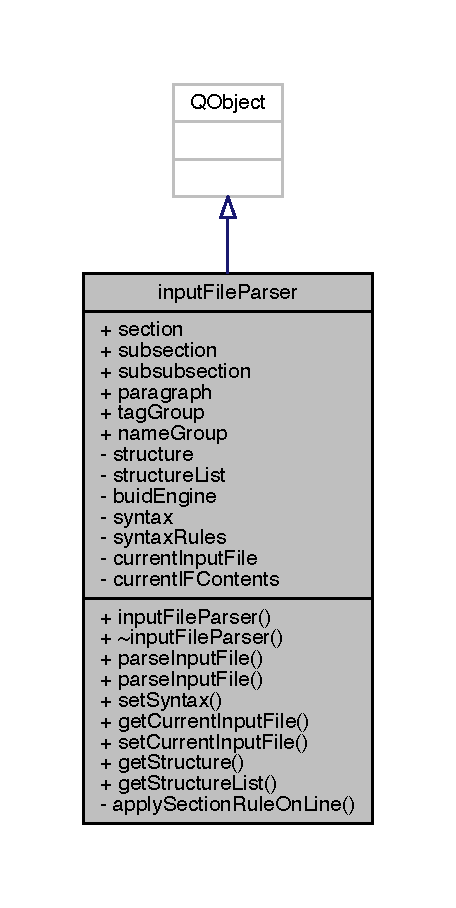
\includegraphics[width=219pt]{classinput_file_parser__inherit__graph}
\end{center}
\end{figure}


Collaboration diagram for input\+File\+Parser\+:\nopagebreak
\begin{figure}[H]
\begin{center}
\leavevmode
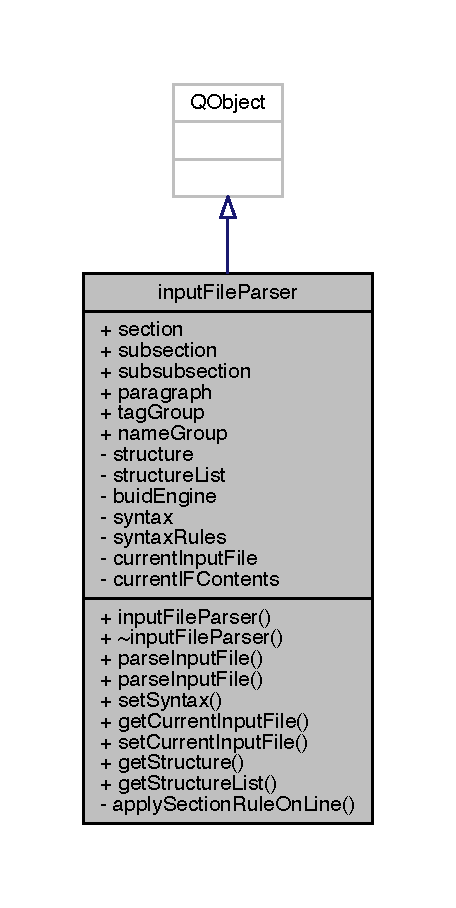
\includegraphics[width=219pt]{classinput_file_parser__coll__graph}
\end{center}
\end{figure}
\subsection*{Public Member Functions}
\begin{DoxyCompactItemize}
\item 
\hyperlink{classinput_file_parser_ad6dae9aa76c40b59ebb5471614815380}{input\+File\+Parser} (Q\+Object $\ast$parent=0)
\item 
\hyperlink{classinput_file_parser_acedec7ed52e2b6222c8cb21844552e9e}{$\sim$input\+File\+Parser} ()
\item 
bool \hyperlink{classinput_file_parser_ad632f2b78c34b72cbaf8105b8762cf9f}{parse\+Input\+File} (Q\+String ifcontents=Q\+String\+::\+Q\+String(\char`\"{}\char`\"{}))
\begin{DoxyCompactList}\small\item\em parse\+Input\+File \end{DoxyCompactList}\item 
bool \hyperlink{classinput_file_parser_a5822704ff80b0fcbfd18f90d0c5d73e9}{parse\+Input\+File} (Q\+File $\ast$ifile)
\begin{DoxyCompactList}\small\item\em parse\+Input\+File \end{DoxyCompactList}\item 
void \hyperlink{classinput_file_parser_afcdec3f3ebb30d601441602e7c6aefe7}{set\+Syntax} (\hyperlink{cdcdefs_8h_ab649dd84a9663b16384131638df4d313}{C\+D\+C\+\_\+file\+Syntax} fsyntax)
\item 
Q\+File $\ast$ \hyperlink{classinput_file_parser_aeba4ba60f2dd40f1e574d57453973904}{get\+Current\+Input\+File} ()
\item 
void \hyperlink{classinput_file_parser_a23af707bf06a90d1e81458415f1d3b96}{set\+Current\+Input\+File} (Q\+File $\ast$value)
\item 
Q\+Standard\+Item\+Model $\ast$ \hyperlink{classinput_file_parser_abd1a6e741e6320d407d8bb4f7d426fff}{get\+Structure} ()
\item 
Q\+List$<$ \hyperlink{struct_c_d_c__doc_structural_element}{C\+D\+C\+\_\+doc\+Structural\+Element} $>$ \hyperlink{classinput_file_parser_ab28a0b22999c9a20ec8c3a72a2c40a7e}{get\+Structure\+List} ()
\end{DoxyCompactItemize}
\subsection*{Private Types}
\begin{DoxyCompactItemize}
\item 
enum \hyperlink{classinput_file_parser_afc7cd4c5ba9e85faf16c9a7b0fec3782}{C\+D\+C\+\_\+p\+States} \{ \\*
\hyperlink{classinput_file_parser_afc7cd4c5ba9e85faf16c9a7b0fec3782aec2f993aec2c27fc750119ab17b16cdb}{C\+D\+C\+\_\+p\+States\+::idle}, 
\hyperlink{classinput_file_parser_afc7cd4c5ba9e85faf16c9a7b0fec3782a12f1613ee9319cfdae1209e5608673fc}{C\+D\+C\+\_\+p\+States\+::at\+\_\+section}, 
\hyperlink{classinput_file_parser_afc7cd4c5ba9e85faf16c9a7b0fec3782a26df3654912116c869d7f61361778779}{C\+D\+C\+\_\+p\+States\+::at\+\_\+subsection}, 
\hyperlink{classinput_file_parser_afc7cd4c5ba9e85faf16c9a7b0fec3782aae921dba06eaa30a3e72e83ad1acfd6f}{C\+D\+C\+\_\+p\+States\+::at\+\_\+subsubsection}, 
\\*
\hyperlink{classinput_file_parser_afc7cd4c5ba9e85faf16c9a7b0fec3782a9588d5dfe50cd47cc712b45d681a4650}{C\+D\+C\+\_\+p\+States\+::at\+\_\+paragraph}
 \}
\begin{DoxyCompactList}\small\item\em Current active input file's contents. \end{DoxyCompactList}\end{DoxyCompactItemize}
\subsection*{Private Member Functions}
\begin{DoxyCompactItemize}
\item 
bool \hyperlink{classinput_file_parser_aede806deb50683f402a34b157b69869f}{apply\+Section\+Rule\+On\+Line} (\hyperlink{cdcdefs_8h_a6116ba1886594c273c61d425c61d6416}{C\+D\+C\+\_\+doc\+Structural\+Element\+Type} type, Q\+String line, int curr\+Line)
\begin{DoxyCompactList}\small\item\em apply\+Section\+Rule\+On\+Line \end{DoxyCompactList}\end{DoxyCompactItemize}
\subsection*{Private Attributes}
\begin{DoxyCompactItemize}
\item 
Q\+Standard\+Item\+Model $\ast$ \hyperlink{classinput_file_parser_ac875012f371d91ecfc383e61f49ed0d4}{structure}
\item 
Q\+List$<$ \hyperlink{struct_c_d_c__doc_structural_element}{C\+D\+C\+\_\+doc\+Structural\+Element} $>$ \hyperlink{classinput_file_parser_a74bd2cbf0855006b5586da0b00c9420b}{structure\+List}
\begin{DoxyCompactList}\small\item\em Structure of the input file (sections, subsecions...) \end{DoxyCompactList}\item 
\hyperlink{cdcdefs_8h_abd38cc943467f0d66216a60454d5ee06}{C\+D\+C\+\_\+build\+Engine} \hyperlink{classinput_file_parser_aa4ec122a74489e07523207b7077a936b}{buid\+Engine}
\item 
\hyperlink{cdcdefs_8h_ab649dd84a9663b16384131638df4d313}{C\+D\+C\+\_\+file\+Syntax} \hyperlink{classinput_file_parser_a9528ecb148895886207571dcaa920626}{syntax}
\item 
\begin{tabbing}
xx\=xx\=xx\=xx\=xx\=xx\=xx\=xx\=xx\=\kill
struct \{\\
\>QRegExp \hyperlink{classinput_file_parser_a7ab3cafcf0f20989346e4d73cc18de88}{section}\\
\>QRegExp \hyperlink{classinput_file_parser_a70c6d19dc97306b9de996ae534198e96}{subsection}\\
\>QRegExp \hyperlink{classinput_file_parser_a3b119638757867ee5fd27f20cbbc56ec}{subsubsection}\\
\>QRegExp \hyperlink{classinput_file_parser_a2701509e686e9c80ff9ca419d4431dad}{paragraph}\\
\>int \hyperlink{classinput_file_parser_ab142598be7ed31c434e5230c3feed1c1}{tagGroup}\\
\>int \hyperlink{classinput_file_parser_a3f70a628f3cfbc541da8b90970f09db3}{nameGroup}\\
\} \hyperlink{classinput_file_parser_a47a7cdb8d77cae8fc1e81e86afb9ff31}{syntaxRules}\\

\end{tabbing}\item 
Q\+File $\ast$ \hyperlink{classinput_file_parser_a09bd8a795ff58263e9afa2ff1200c4cc}{current\+Input\+File}
\item 
Q\+String \hyperlink{classinput_file_parser_a112d1bd30d2093be8eb76ed02333a322}{current\+I\+F\+Contents}
\begin{DoxyCompactList}\small\item\em Handle to the current input file. \end{DoxyCompactList}\end{DoxyCompactItemize}


\subsection{Detailed Description}


Definition at line 34 of file inputfileparser.\+h.



\subsection{Member Enumeration Documentation}
\hypertarget{classinput_file_parser_afc7cd4c5ba9e85faf16c9a7b0fec3782}{\index{input\+File\+Parser@{input\+File\+Parser}!C\+D\+C\+\_\+p\+States@{C\+D\+C\+\_\+p\+States}}
\index{C\+D\+C\+\_\+p\+States@{C\+D\+C\+\_\+p\+States}!input\+File\+Parser@{input\+File\+Parser}}
\subsubsection[{C\+D\+C\+\_\+p\+States}]{\setlength{\rightskip}{0pt plus 5cm}enum {\bf input\+File\+Parser\+::\+C\+D\+C\+\_\+p\+States}\hspace{0.3cm}{\ttfamily [strong]}, {\ttfamily [private]}}}\label{classinput_file_parser_afc7cd4c5ba9e85faf16c9a7b0fec3782}


Current active input file's contents. 

States for the parsing state machine \begin{Desc}
\item[Enumerator]\par
\begin{description}
\index{idle@{idle}!input\+File\+Parser@{input\+File\+Parser}}\index{input\+File\+Parser@{input\+File\+Parser}!idle@{idle}}\item[{\em 
\hypertarget{classinput_file_parser_afc7cd4c5ba9e85faf16c9a7b0fec3782aec2f993aec2c27fc750119ab17b16cdb}{idle}\label{classinput_file_parser_afc7cd4c5ba9e85faf16c9a7b0fec3782aec2f993aec2c27fc750119ab17b16cdb}
}]\index{at\+\_\+section@{at\+\_\+section}!input\+File\+Parser@{input\+File\+Parser}}\index{input\+File\+Parser@{input\+File\+Parser}!at\+\_\+section@{at\+\_\+section}}\item[{\em 
\hypertarget{classinput_file_parser_afc7cd4c5ba9e85faf16c9a7b0fec3782a12f1613ee9319cfdae1209e5608673fc}{at\+\_\+section}\label{classinput_file_parser_afc7cd4c5ba9e85faf16c9a7b0fec3782a12f1613ee9319cfdae1209e5608673fc}
}]Didn't find anything. \index{at\+\_\+subsection@{at\+\_\+subsection}!input\+File\+Parser@{input\+File\+Parser}}\index{input\+File\+Parser@{input\+File\+Parser}!at\+\_\+subsection@{at\+\_\+subsection}}\item[{\em 
\hypertarget{classinput_file_parser_afc7cd4c5ba9e85faf16c9a7b0fec3782a26df3654912116c869d7f61361778779}{at\+\_\+subsection}\label{classinput_file_parser_afc7cd4c5ba9e85faf16c9a7b0fec3782a26df3654912116c869d7f61361778779}
}]Found a section header. Will append subsections to it, if any. \index{at\+\_\+subsubsection@{at\+\_\+subsubsection}!input\+File\+Parser@{input\+File\+Parser}}\index{input\+File\+Parser@{input\+File\+Parser}!at\+\_\+subsubsection@{at\+\_\+subsubsection}}\item[{\em 
\hypertarget{classinput_file_parser_afc7cd4c5ba9e85faf16c9a7b0fec3782aae921dba06eaa30a3e72e83ad1acfd6f}{at\+\_\+subsubsection}\label{classinput_file_parser_afc7cd4c5ba9e85faf16c9a7b0fec3782aae921dba06eaa30a3e72e83ad1acfd6f}
}]Found a subsection header. Will append subsubsections to it, if any. \index{at\+\_\+paragraph@{at\+\_\+paragraph}!input\+File\+Parser@{input\+File\+Parser}}\index{input\+File\+Parser@{input\+File\+Parser}!at\+\_\+paragraph@{at\+\_\+paragraph}}\item[{\em 
\hypertarget{classinput_file_parser_afc7cd4c5ba9e85faf16c9a7b0fec3782a9588d5dfe50cd47cc712b45d681a4650}{at\+\_\+paragraph}\label{classinput_file_parser_afc7cd4c5ba9e85faf16c9a7b0fec3782a9588d5dfe50cd47cc712b45d681a4650}
}]Found a subsubsection header. Will append paragraphs to it, if any. Found a paragraph header \end{description}
\end{Desc}


Definition at line 85 of file inputfileparser.\+h.



\subsection{Constructor \& Destructor Documentation}
\hypertarget{classinput_file_parser_ad6dae9aa76c40b59ebb5471614815380}{\index{input\+File\+Parser@{input\+File\+Parser}!input\+File\+Parser@{input\+File\+Parser}}
\index{input\+File\+Parser@{input\+File\+Parser}!input\+File\+Parser@{input\+File\+Parser}}
\subsubsection[{input\+File\+Parser}]{\setlength{\rightskip}{0pt plus 5cm}input\+File\+Parser\+::input\+File\+Parser (
\begin{DoxyParamCaption}
\item[{Q\+Object $\ast$}]{parent = {\ttfamily 0}}
\end{DoxyParamCaption}
)}}\label{classinput_file_parser_ad6dae9aa76c40b59ebb5471614815380}


Definition at line 22 of file inputfileparser.\+cpp.

\hypertarget{classinput_file_parser_acedec7ed52e2b6222c8cb21844552e9e}{\index{input\+File\+Parser@{input\+File\+Parser}!````~input\+File\+Parser@{$\sim$input\+File\+Parser}}
\index{````~input\+File\+Parser@{$\sim$input\+File\+Parser}!input\+File\+Parser@{input\+File\+Parser}}
\subsubsection[{$\sim$input\+File\+Parser}]{\setlength{\rightskip}{0pt plus 5cm}input\+File\+Parser\+::$\sim$input\+File\+Parser (
\begin{DoxyParamCaption}
{}
\end{DoxyParamCaption}
)}}\label{classinput_file_parser_acedec7ed52e2b6222c8cb21844552e9e}


Definition at line 28 of file inputfileparser.\+cpp.



\subsection{Member Function Documentation}
\hypertarget{classinput_file_parser_aede806deb50683f402a34b157b69869f}{\index{input\+File\+Parser@{input\+File\+Parser}!apply\+Section\+Rule\+On\+Line@{apply\+Section\+Rule\+On\+Line}}
\index{apply\+Section\+Rule\+On\+Line@{apply\+Section\+Rule\+On\+Line}!input\+File\+Parser@{input\+File\+Parser}}
\subsubsection[{apply\+Section\+Rule\+On\+Line}]{\setlength{\rightskip}{0pt plus 5cm}bool input\+File\+Parser\+::apply\+Section\+Rule\+On\+Line (
\begin{DoxyParamCaption}
\item[{{\bf C\+D\+C\+\_\+doc\+Structural\+Element\+Type}}]{type, }
\item[{Q\+String}]{line, }
\item[{int}]{curr\+Line}
\end{DoxyParamCaption}
)\hspace{0.3cm}{\ttfamily [private]}}}\label{classinput_file_parser_aede806deb50683f402a34b157b69869f}


apply\+Section\+Rule\+On\+Line 


\begin{DoxyParams}{Parameters}
{\em type} & \\
\hline
{\em line} & \\
\hline
\end{DoxyParams}
\begin{DoxyReturn}{Returns}
If the desired section was found in that particular line. 
\end{DoxyReturn}


Definition at line 123 of file inputfileparser.\+cpp.

\hypertarget{classinput_file_parser_aeba4ba60f2dd40f1e574d57453973904}{\index{input\+File\+Parser@{input\+File\+Parser}!get\+Current\+Input\+File@{get\+Current\+Input\+File}}
\index{get\+Current\+Input\+File@{get\+Current\+Input\+File}!input\+File\+Parser@{input\+File\+Parser}}
\subsubsection[{get\+Current\+Input\+File}]{\setlength{\rightskip}{0pt plus 5cm}Q\+File$\ast$ input\+File\+Parser\+::get\+Current\+Input\+File (
\begin{DoxyParamCaption}
{}
\end{DoxyParamCaption}
)\hspace{0.3cm}{\ttfamily [inline]}}}\label{classinput_file_parser_aeba4ba60f2dd40f1e574d57453973904}


Definition at line 57 of file inputfileparser.\+h.

\hypertarget{classinput_file_parser_abd1a6e741e6320d407d8bb4f7d426fff}{\index{input\+File\+Parser@{input\+File\+Parser}!get\+Structure@{get\+Structure}}
\index{get\+Structure@{get\+Structure}!input\+File\+Parser@{input\+File\+Parser}}
\subsubsection[{get\+Structure}]{\setlength{\rightskip}{0pt plus 5cm}Q\+Standard\+Item\+Model$\ast$ input\+File\+Parser\+::get\+Structure (
\begin{DoxyParamCaption}
{}
\end{DoxyParamCaption}
)\hspace{0.3cm}{\ttfamily [inline]}}}\label{classinput_file_parser_abd1a6e741e6320d407d8bb4f7d426fff}


Definition at line 60 of file inputfileparser.\+h.

\hypertarget{classinput_file_parser_ab28a0b22999c9a20ec8c3a72a2c40a7e}{\index{input\+File\+Parser@{input\+File\+Parser}!get\+Structure\+List@{get\+Structure\+List}}
\index{get\+Structure\+List@{get\+Structure\+List}!input\+File\+Parser@{input\+File\+Parser}}
\subsubsection[{get\+Structure\+List}]{\setlength{\rightskip}{0pt plus 5cm}Q\+List$<${\bf C\+D\+C\+\_\+doc\+Structural\+Element}$>$ input\+File\+Parser\+::get\+Structure\+List (
\begin{DoxyParamCaption}
{}
\end{DoxyParamCaption}
)\hspace{0.3cm}{\ttfamily [inline]}}}\label{classinput_file_parser_ab28a0b22999c9a20ec8c3a72a2c40a7e}


Definition at line 62 of file inputfileparser.\+h.

\hypertarget{classinput_file_parser_ad632f2b78c34b72cbaf8105b8762cf9f}{\index{input\+File\+Parser@{input\+File\+Parser}!parse\+Input\+File@{parse\+Input\+File}}
\index{parse\+Input\+File@{parse\+Input\+File}!input\+File\+Parser@{input\+File\+Parser}}
\subsubsection[{parse\+Input\+File}]{\setlength{\rightskip}{0pt plus 5cm}bool input\+File\+Parser\+::parse\+Input\+File (
\begin{DoxyParamCaption}
\item[{Q\+String}]{ifcontents = {\ttfamily QString\+:\+:QString(\char`\"{}\char`\"{})}}
\end{DoxyParamCaption}
)}}\label{classinput_file_parser_ad632f2b78c34b72cbaf8105b8762cf9f}


parse\+Input\+File 


\begin{DoxyParams}{Parameters}
{\em ifcontents} & \\
\hline
\end{DoxyParams}
\begin{DoxyReturn}{Returns}

\end{DoxyReturn}


Definition at line 46 of file inputfileparser.\+cpp.

\hypertarget{classinput_file_parser_a5822704ff80b0fcbfd18f90d0c5d73e9}{\index{input\+File\+Parser@{input\+File\+Parser}!parse\+Input\+File@{parse\+Input\+File}}
\index{parse\+Input\+File@{parse\+Input\+File}!input\+File\+Parser@{input\+File\+Parser}}
\subsubsection[{parse\+Input\+File}]{\setlength{\rightskip}{0pt plus 5cm}bool input\+File\+Parser\+::parse\+Input\+File (
\begin{DoxyParamCaption}
\item[{Q\+File $\ast$}]{ifile}
\end{DoxyParamCaption}
)}}\label{classinput_file_parser_a5822704ff80b0fcbfd18f90d0c5d73e9}


parse\+Input\+File 


\begin{DoxyParams}{Parameters}
{\em ifile} & \\
\hline
\end{DoxyParams}
\begin{DoxyReturn}{Returns}

\end{DoxyReturn}


Definition at line 36 of file inputfileparser.\+cpp.

\hypertarget{classinput_file_parser_a23af707bf06a90d1e81458415f1d3b96}{\index{input\+File\+Parser@{input\+File\+Parser}!set\+Current\+Input\+File@{set\+Current\+Input\+File}}
\index{set\+Current\+Input\+File@{set\+Current\+Input\+File}!input\+File\+Parser@{input\+File\+Parser}}
\subsubsection[{set\+Current\+Input\+File}]{\setlength{\rightskip}{0pt plus 5cm}void input\+File\+Parser\+::set\+Current\+Input\+File (
\begin{DoxyParamCaption}
\item[{Q\+File $\ast$}]{value}
\end{DoxyParamCaption}
)\hspace{0.3cm}{\ttfamily [inline]}}}\label{classinput_file_parser_a23af707bf06a90d1e81458415f1d3b96}


Definition at line 58 of file inputfileparser.\+h.

\hypertarget{classinput_file_parser_afcdec3f3ebb30d601441602e7c6aefe7}{\index{input\+File\+Parser@{input\+File\+Parser}!set\+Syntax@{set\+Syntax}}
\index{set\+Syntax@{set\+Syntax}!input\+File\+Parser@{input\+File\+Parser}}
\subsubsection[{set\+Syntax}]{\setlength{\rightskip}{0pt plus 5cm}void input\+File\+Parser\+::set\+Syntax (
\begin{DoxyParamCaption}
\item[{{\bf C\+D\+C\+\_\+file\+Syntax}}]{fsyntax}
\end{DoxyParamCaption}
)}}\label{classinput_file_parser_afcdec3f3ebb30d601441602e7c6aefe7}


Definition at line 103 of file inputfileparser.\+cpp.



\subsection{Member Data Documentation}
\hypertarget{classinput_file_parser_aa4ec122a74489e07523207b7077a936b}{\index{input\+File\+Parser@{input\+File\+Parser}!buid\+Engine@{buid\+Engine}}
\index{buid\+Engine@{buid\+Engine}!input\+File\+Parser@{input\+File\+Parser}}
\subsubsection[{buid\+Engine}]{\setlength{\rightskip}{0pt plus 5cm}{\bf C\+D\+C\+\_\+build\+Engine} input\+File\+Parser\+::buid\+Engine\hspace{0.3cm}{\ttfamily [private]}}}\label{classinput_file_parser_aa4ec122a74489e07523207b7077a936b}


Definition at line 69 of file inputfileparser.\+h.

\hypertarget{classinput_file_parser_a112d1bd30d2093be8eb76ed02333a322}{\index{input\+File\+Parser@{input\+File\+Parser}!current\+I\+F\+Contents@{current\+I\+F\+Contents}}
\index{current\+I\+F\+Contents@{current\+I\+F\+Contents}!input\+File\+Parser@{input\+File\+Parser}}
\subsubsection[{current\+I\+F\+Contents}]{\setlength{\rightskip}{0pt plus 5cm}Q\+String input\+File\+Parser\+::current\+I\+F\+Contents\hspace{0.3cm}{\ttfamily [private]}}}\label{classinput_file_parser_a112d1bd30d2093be8eb76ed02333a322}


Handle to the current input file. 



Definition at line 82 of file inputfileparser.\+h.

\hypertarget{classinput_file_parser_a09bd8a795ff58263e9afa2ff1200c4cc}{\index{input\+File\+Parser@{input\+File\+Parser}!current\+Input\+File@{current\+Input\+File}}
\index{current\+Input\+File@{current\+Input\+File}!input\+File\+Parser@{input\+File\+Parser}}
\subsubsection[{current\+Input\+File}]{\setlength{\rightskip}{0pt plus 5cm}Q\+File$\ast$ input\+File\+Parser\+::current\+Input\+File\hspace{0.3cm}{\ttfamily [private]}}}\label{classinput_file_parser_a09bd8a795ff58263e9afa2ff1200c4cc}


Definition at line 81 of file inputfileparser.\+h.

\hypertarget{classinput_file_parser_a3f70a628f3cfbc541da8b90970f09db3}{\index{input\+File\+Parser@{input\+File\+Parser}!name\+Group@{name\+Group}}
\index{name\+Group@{name\+Group}!input\+File\+Parser@{input\+File\+Parser}}
\subsubsection[{name\+Group}]{\setlength{\rightskip}{0pt plus 5cm}int input\+File\+Parser\+::name\+Group}}\label{classinput_file_parser_a3f70a628f3cfbc541da8b90970f09db3}


Definition at line 78 of file inputfileparser.\+h.

\hypertarget{classinput_file_parser_a2701509e686e9c80ff9ca419d4431dad}{\index{input\+File\+Parser@{input\+File\+Parser}!paragraph@{paragraph}}
\index{paragraph@{paragraph}!input\+File\+Parser@{input\+File\+Parser}}
\subsubsection[{paragraph}]{\setlength{\rightskip}{0pt plus 5cm}Q\+Reg\+Exp input\+File\+Parser\+::paragraph}}\label{classinput_file_parser_a2701509e686e9c80ff9ca419d4431dad}


Definition at line 76 of file inputfileparser.\+h.

\hypertarget{classinput_file_parser_a7ab3cafcf0f20989346e4d73cc18de88}{\index{input\+File\+Parser@{input\+File\+Parser}!section@{section}}
\index{section@{section}!input\+File\+Parser@{input\+File\+Parser}}
\subsubsection[{section}]{\setlength{\rightskip}{0pt plus 5cm}Q\+Reg\+Exp input\+File\+Parser\+::section}}\label{classinput_file_parser_a7ab3cafcf0f20989346e4d73cc18de88}


Definition at line 73 of file inputfileparser.\+h.

\hypertarget{classinput_file_parser_ac875012f371d91ecfc383e61f49ed0d4}{\index{input\+File\+Parser@{input\+File\+Parser}!structure@{structure}}
\index{structure@{structure}!input\+File\+Parser@{input\+File\+Parser}}
\subsubsection[{structure}]{\setlength{\rightskip}{0pt plus 5cm}Q\+Standard\+Item\+Model$\ast$ input\+File\+Parser\+::structure\hspace{0.3cm}{\ttfamily [private]}}}\label{classinput_file_parser_ac875012f371d91ecfc383e61f49ed0d4}


Definition at line 65 of file inputfileparser.\+h.

\hypertarget{classinput_file_parser_a74bd2cbf0855006b5586da0b00c9420b}{\index{input\+File\+Parser@{input\+File\+Parser}!structure\+List@{structure\+List}}
\index{structure\+List@{structure\+List}!input\+File\+Parser@{input\+File\+Parser}}
\subsubsection[{structure\+List}]{\setlength{\rightskip}{0pt plus 5cm}Q\+List$<${\bf C\+D\+C\+\_\+doc\+Structural\+Element}$>$ input\+File\+Parser\+::structure\+List\hspace{0.3cm}{\ttfamily [private]}}}\label{classinput_file_parser_a74bd2cbf0855006b5586da0b00c9420b}


Structure of the input file (sections, subsecions...) 



Definition at line 67 of file inputfileparser.\+h.

\hypertarget{classinput_file_parser_a70c6d19dc97306b9de996ae534198e96}{\index{input\+File\+Parser@{input\+File\+Parser}!subsection@{subsection}}
\index{subsection@{subsection}!input\+File\+Parser@{input\+File\+Parser}}
\subsubsection[{subsection}]{\setlength{\rightskip}{0pt plus 5cm}Q\+Reg\+Exp input\+File\+Parser\+::subsection}}\label{classinput_file_parser_a70c6d19dc97306b9de996ae534198e96}


Definition at line 74 of file inputfileparser.\+h.

\hypertarget{classinput_file_parser_a3b119638757867ee5fd27f20cbbc56ec}{\index{input\+File\+Parser@{input\+File\+Parser}!subsubsection@{subsubsection}}
\index{subsubsection@{subsubsection}!input\+File\+Parser@{input\+File\+Parser}}
\subsubsection[{subsubsection}]{\setlength{\rightskip}{0pt plus 5cm}Q\+Reg\+Exp input\+File\+Parser\+::subsubsection}}\label{classinput_file_parser_a3b119638757867ee5fd27f20cbbc56ec}


Definition at line 75 of file inputfileparser.\+h.

\hypertarget{classinput_file_parser_a9528ecb148895886207571dcaa920626}{\index{input\+File\+Parser@{input\+File\+Parser}!syntax@{syntax}}
\index{syntax@{syntax}!input\+File\+Parser@{input\+File\+Parser}}
\subsubsection[{syntax}]{\setlength{\rightskip}{0pt plus 5cm}{\bf C\+D\+C\+\_\+file\+Syntax} input\+File\+Parser\+::syntax\hspace{0.3cm}{\ttfamily [private]}}}\label{classinput_file_parser_a9528ecb148895886207571dcaa920626}


Definition at line 70 of file inputfileparser.\+h.

\hypertarget{classinput_file_parser_a47a7cdb8d77cae8fc1e81e86afb9ff31}{\index{input\+File\+Parser@{input\+File\+Parser}!syntax\+Rules@{syntax\+Rules}}
\index{syntax\+Rules@{syntax\+Rules}!input\+File\+Parser@{input\+File\+Parser}}
\subsubsection[{syntax\+Rules}]{\setlength{\rightskip}{0pt plus 5cm}struct \{ ... \}   input\+File\+Parser\+::syntax\+Rules\hspace{0.3cm}{\ttfamily [private]}}}\label{classinput_file_parser_a47a7cdb8d77cae8fc1e81e86afb9ff31}
\hypertarget{classinput_file_parser_ab142598be7ed31c434e5230c3feed1c1}{\index{input\+File\+Parser@{input\+File\+Parser}!tag\+Group@{tag\+Group}}
\index{tag\+Group@{tag\+Group}!input\+File\+Parser@{input\+File\+Parser}}
\subsubsection[{tag\+Group}]{\setlength{\rightskip}{0pt plus 5cm}int input\+File\+Parser\+::tag\+Group}}\label{classinput_file_parser_ab142598be7ed31c434e5230c3feed1c1}


Definition at line 77 of file inputfileparser.\+h.



The documentation for this class was generated from the following files\+:\begin{DoxyCompactItemize}
\item 
/\+Users/martin/\+Workspaces/qt/crossdocs\+\_\+gui/\hyperlink{inputfileparser_8h}{inputfileparser.\+h}\item 
/\+Users/martin/\+Workspaces/qt/crossdocs\+\_\+gui/\hyperlink{inputfileparser_8cpp}{inputfileparser.\+cpp}\end{DoxyCompactItemize}

\hypertarget{classproject_worker}{\section{project\+Worker Class Reference}
\label{classproject_worker}\index{project\+Worker@{project\+Worker}}
}


{\ttfamily \#include $<$projectworker.\+h$>$}



Inheritance diagram for project\+Worker\+:\nopagebreak
\begin{figure}[H]
\begin{center}
\leavevmode
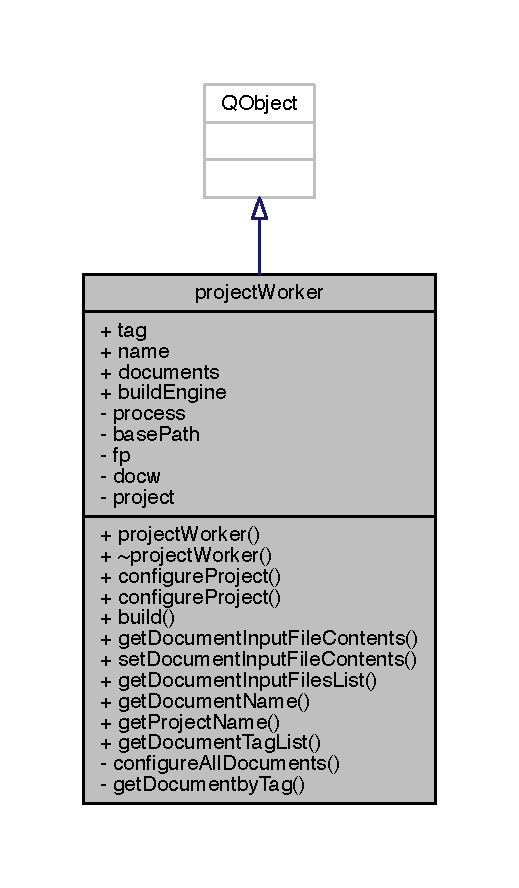
\includegraphics[width=249pt]{classproject_worker__inherit__graph}
\end{center}
\end{figure}


Collaboration diagram for project\+Worker\+:\nopagebreak
\begin{figure}[H]
\begin{center}
\leavevmode
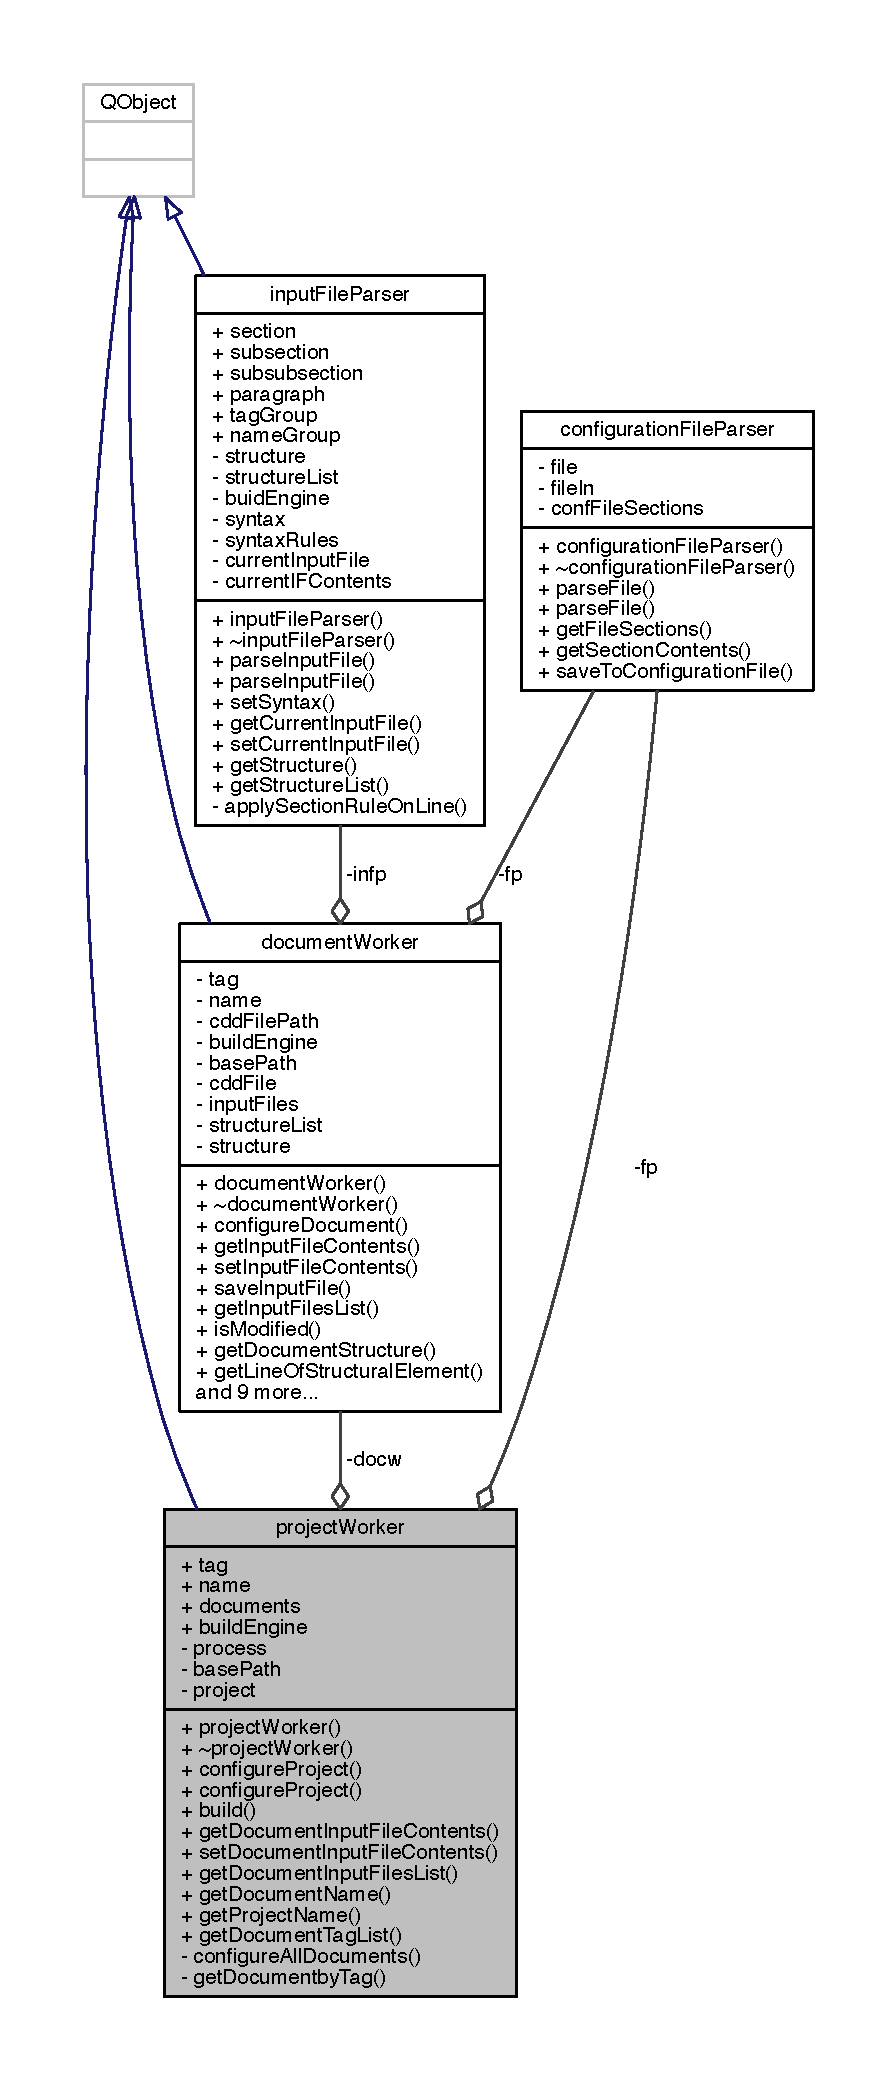
\includegraphics[height=550pt]{classproject_worker__coll__graph}
\end{center}
\end{figure}
\subsection*{Public Member Functions}
\begin{DoxyCompactItemize}
\item 
\hyperlink{classproject_worker_a1fc4d7a88361b1f46232f7839f9ed40f}{project\+Worker} (Q\+Object $\ast$parent=0)
\item 
\hyperlink{classproject_worker_a584073fedfbbc9465ae1bdb16c9187f0}{$\sim$project\+Worker} ()
\item 
bool \hyperlink{classproject_worker_a1693b92f8d27a4487eb58827c6741de8}{configure\+Project} (Q\+String prjconffile, \hyperlink{cdcdefs_8h_a7a1ca742b5a041762c1b5784532bd7fd}{C\+D\+C\+\_\+status} $\ast$ret\+Status=N\+U\+L\+L)
\begin{DoxyCompactList}\small\item\em Runs \hyperlink{classconfiguration_file_parser}{configuration\+File\+Parser} on prjconffile and builds internal project model. \end{DoxyCompactList}\item 
bool \hyperlink{classproject_worker_a3674849ec41f25950e60277bdc2e1a68}{configure\+Project} (Q\+Dir pcf, \hyperlink{cdcdefs_8h_a7a1ca742b5a041762c1b5784532bd7fd}{C\+D\+C\+\_\+status} $\ast$r\+St=N\+U\+L\+L)
\item 
bool \hyperlink{classproject_worker_ae616cf4cb8461ef98b9f13e25751e5a8}{build} (Q\+String prjconffile=Q\+String\+::\+Q\+String(\char`\"{}\char`\"{}), \hyperlink{cdcdefs_8h_a7a1ca742b5a041762c1b5784532bd7fd}{C\+D\+C\+\_\+status} $\ast$ret\+Status=N\+U\+L\+L)
\item 
Q\+String \hyperlink{classproject_worker_ac9c8f8d67e7968c3537d0a8b78362706}{get\+Document\+Input\+File\+Contents} (Q\+String doctag, int if\+Index, \hyperlink{cdcdefs_8h_a7a1ca742b5a041762c1b5784532bd7fd}{C\+D\+C\+\_\+status} $\ast$ret\+Status=N\+U\+L\+L)
\begin{DoxyCompactList}\small\item\em Returns the contents of a certain input file from a document. \end{DoxyCompactList}\item 
void \hyperlink{classproject_worker_ae5f11f2acab566dc8a55eb758ba94834}{set\+Document\+Input\+File\+Contents} (Q\+String doctag, int if\+Index, Q\+String content, \hyperlink{cdcdefs_8h_a7a1ca742b5a041762c1b5784532bd7fd}{C\+D\+C\+\_\+status} $\ast$ret\+Status=N\+U\+L\+L)
\begin{DoxyCompactList}\small\item\em Changes the contents of the input file from a document. Also checks if this input file is referenced by more than one document, and updates all references. Check also \hyperlink{classdocument_worker_aefcc1bfe56d564865818ded4b258c20e}{document\+Worker\+::get\+Input\+File\+Contents()} . \end{DoxyCompactList}\item 
Q\+String\+List \hyperlink{classproject_worker_a87e5d67dc1b313ab1d0a0f48f20fbabf}{get\+Document\+Input\+Files\+List} (Q\+String doctag)
\item 
Q\+String \hyperlink{classproject_worker_aacc955ad8a4a700e677f02322d457e5c}{get\+Document\+Name} (Q\+String doctag)
\item 
Q\+String \hyperlink{classproject_worker_a111a4e4aa9a87786819792d06047fa71}{get\+Project\+Name} ()
\item 
Q\+String\+List \hyperlink{classproject_worker_aa90487309a19fddcf97555ac783089b9}{get\+Document\+Tag\+List} ()
\end{DoxyCompactItemize}
\subsection*{Private Member Functions}
\begin{DoxyCompactItemize}
\item 
bool \hyperlink{classproject_worker_a98cedd223de4c9507a6c1b0bf05eb1e6}{configure\+All\+Documents} ()
\begin{DoxyCompactList}\small\item\em Configures all documents already in the project strucutre. If one (or more) document fails to parse, the function will carry on parsing all the other docs, but will return false nontheless. \end{DoxyCompactList}\item 
\hyperlink{classdocument_worker}{document\+Worker} $\ast$ \hyperlink{classproject_worker_a11b102e3b0ae2d129aed9a2e105ff8f4}{get\+Documentby\+Tag} (Q\+String \hyperlink{classproject_worker_aba02c11fc0a014e1743feff1d8347ad2}{tag})
\begin{DoxyCompactList}\small\item\em Returns the pointer to the project's document with the specified tag. Internal function that is used as general document getter for all other indirect document manipultions. \end{DoxyCompactList}\end{DoxyCompactItemize}
\subsection*{Private Attributes}
\begin{DoxyCompactItemize}
\item 
Q\+Process $\ast$ \hyperlink{classproject_worker_a862f3fc1a316f1542e843281e2667344}{process}
\item 
Q\+String \hyperlink{classproject_worker_acebb1a43f3056c7bb74bfe8d6bd0411e}{base\+Path}
\item 
\hyperlink{classconfiguration_file_parser}{configuration\+File\+Parser} $\ast$ \hyperlink{classproject_worker_a3e67d186faa22b7cfa338ae9e0272da0}{fp}
\item 
\hyperlink{classdocument_worker}{document\+Worker} $\ast$ \hyperlink{classproject_worker_a5bd23894e1f09311b4bebcd92c644e8b}{docw}
\item 
\begin{tabbing}
xx\=xx\=xx\=xx\=xx\=xx\=xx\=xx\=xx\=\kill
struct \{\\
\>QString \hyperlink{classproject_worker_aba02c11fc0a014e1743feff1d8347ad2}{tag}\\
\>QString \hyperlink{classproject_worker_a133798ef8a45a15919e4f65e2bb3df71}{name}\\
\>QList$<$ \hyperlink{classdocument_worker}{documentWorker} $\ast$ $>$ \hyperlink{classproject_worker_acdd055f2642057c2766e0aeded1237c5}{documents}\\
\>\hyperlink{cdcdefs_8h_abd38cc943467f0d66216a60454d5ee06}{CDC\_buildEngine} \hyperlink{classproject_worker_a88c5f6033c06ee66f102642cfe32497c}{buildEngine}\\
\} \hyperlink{classproject_worker_a1e4589fdd07b5d6063e703b211dd8aa9}{project}\\

\end{tabbing}\begin{DoxyCompactList}\small\item\em Struct that contains the current project's params. Only one prj at a time. \end{DoxyCompactList}\end{DoxyCompactItemize}


\subsection{Detailed Description}


Definition at line 36 of file projectworker.\+h.



\subsection{Constructor \& Destructor Documentation}
\hypertarget{classproject_worker_a1fc4d7a88361b1f46232f7839f9ed40f}{\index{project\+Worker@{project\+Worker}!project\+Worker@{project\+Worker}}
\index{project\+Worker@{project\+Worker}!project\+Worker@{project\+Worker}}
\subsubsection[{project\+Worker}]{\setlength{\rightskip}{0pt plus 5cm}project\+Worker\+::project\+Worker (
\begin{DoxyParamCaption}
\item[{Q\+Object $\ast$}]{parent = {\ttfamily 0}}
\end{DoxyParamCaption}
)}}\label{classproject_worker_a1fc4d7a88361b1f46232f7839f9ed40f}


Definition at line 28 of file projectworker.\+cpp.

\hypertarget{classproject_worker_a584073fedfbbc9465ae1bdb16c9187f0}{\index{project\+Worker@{project\+Worker}!````~project\+Worker@{$\sim$project\+Worker}}
\index{````~project\+Worker@{$\sim$project\+Worker}!project\+Worker@{project\+Worker}}
\subsubsection[{$\sim$project\+Worker}]{\setlength{\rightskip}{0pt plus 5cm}project\+Worker\+::$\sim$project\+Worker (
\begin{DoxyParamCaption}
{}
\end{DoxyParamCaption}
)}}\label{classproject_worker_a584073fedfbbc9465ae1bdb16c9187f0}


Definition at line 35 of file projectworker.\+cpp.



\subsection{Member Function Documentation}
\hypertarget{classproject_worker_ae616cf4cb8461ef98b9f13e25751e5a8}{\index{project\+Worker@{project\+Worker}!build@{build}}
\index{build@{build}!project\+Worker@{project\+Worker}}
\subsubsection[{build}]{\setlength{\rightskip}{0pt plus 5cm}bool project\+Worker\+::build (
\begin{DoxyParamCaption}
\item[{Q\+String}]{prjconffile = {\ttfamily QString\+:\+:QString(\char`\"{}\char`\"{})}, }
\item[{{\bf C\+D\+C\+\_\+status} $\ast$}]{ret\+Status = {\ttfamily NULL}}
\end{DoxyParamCaption}
)}}\label{classproject_worker_ae616cf4cb8461ef98b9f13e25751e5a8}


Definition at line 125 of file projectworker.\+cpp.

\hypertarget{classproject_worker_a98cedd223de4c9507a6c1b0bf05eb1e6}{\index{project\+Worker@{project\+Worker}!configure\+All\+Documents@{configure\+All\+Documents}}
\index{configure\+All\+Documents@{configure\+All\+Documents}!project\+Worker@{project\+Worker}}
\subsubsection[{configure\+All\+Documents}]{\setlength{\rightskip}{0pt plus 5cm}bool project\+Worker\+::configure\+All\+Documents (
\begin{DoxyParamCaption}
{}
\end{DoxyParamCaption}
)\hspace{0.3cm}{\ttfamily [private]}}}\label{classproject_worker_a98cedd223de4c9507a6c1b0bf05eb1e6}


Configures all documents already in the project strucutre. If one (or more) document fails to parse, the function will carry on parsing all the other docs, but will return false nontheless. 

\begin{DoxyReturn}{Returns}
Whether parse went ok. Return false if at least one document failed to parse. 
\end{DoxyReturn}


Definition at line 178 of file projectworker.\+cpp.

\hypertarget{classproject_worker_a1693b92f8d27a4487eb58827c6741de8}{\index{project\+Worker@{project\+Worker}!configure\+Project@{configure\+Project}}
\index{configure\+Project@{configure\+Project}!project\+Worker@{project\+Worker}}
\subsubsection[{configure\+Project}]{\setlength{\rightskip}{0pt plus 5cm}bool project\+Worker\+::configure\+Project (
\begin{DoxyParamCaption}
\item[{Q\+String}]{prjconffile, }
\item[{{\bf C\+D\+C\+\_\+status} $\ast$}]{ret\+Status = {\ttfamily NULL}}
\end{DoxyParamCaption}
)}}\label{classproject_worker_a1693b92f8d27a4487eb58827c6741de8}


Runs \hyperlink{classconfiguration_file_parser}{configuration\+File\+Parser} on prjconffile and builds internal project model. 


\begin{DoxyParams}{Parameters}
{\em prjconffile} & {\bfseries Q\+String} containing the full path to the configuration file. \\
\hline
{\em ret\+Status} & C\+D\+C\+\_\+status of the operation. \\
\hline
\end{DoxyParams}
\begin{DoxyReturn}{Returns}
Whether parse went ok (\hyperlink{cdcdefs_8h_a7a1ca742b5a041762c1b5784532bd7fda444bcb3a3fcf8389296c49467f27e1d6}{C\+D\+C\+\_\+status\+::ok}). 
\end{DoxyReturn}


Definition at line 44 of file projectworker.\+cpp.

\hypertarget{classproject_worker_a3674849ec41f25950e60277bdc2e1a68}{\index{project\+Worker@{project\+Worker}!configure\+Project@{configure\+Project}}
\index{configure\+Project@{configure\+Project}!project\+Worker@{project\+Worker}}
\subsubsection[{configure\+Project}]{\setlength{\rightskip}{0pt plus 5cm}bool project\+Worker\+::configure\+Project (
\begin{DoxyParamCaption}
\item[{Q\+Dir}]{pcf, }
\item[{{\bf C\+D\+C\+\_\+status} $\ast$}]{r\+St = {\ttfamily NULL}}
\end{DoxyParamCaption}
)\hspace{0.3cm}{\ttfamily [inline]}}}\label{classproject_worker_a3674849ec41f25950e60277bdc2e1a68}


Definition at line 51 of file projectworker.\+h.

\hypertarget{classproject_worker_a11b102e3b0ae2d129aed9a2e105ff8f4}{\index{project\+Worker@{project\+Worker}!get\+Documentby\+Tag@{get\+Documentby\+Tag}}
\index{get\+Documentby\+Tag@{get\+Documentby\+Tag}!project\+Worker@{project\+Worker}}
\subsubsection[{get\+Documentby\+Tag}]{\setlength{\rightskip}{0pt plus 5cm}{\bf document\+Worker} $\ast$ project\+Worker\+::get\+Documentby\+Tag (
\begin{DoxyParamCaption}
\item[{Q\+String}]{tag}
\end{DoxyParamCaption}
)\hspace{0.3cm}{\ttfamily [private]}}}\label{classproject_worker_a11b102e3b0ae2d129aed9a2e105ff8f4}


Returns the pointer to the project's document with the specified tag. Internal function that is used as general document getter for all other indirect document manipultions. 


\begin{DoxyParams}{Parameters}
{\em tag} & Tag of the desired document. \\
\hline
\end{DoxyParams}
\begin{DoxyReturn}{Returns}
Pointer to the \hyperlink{classdocument_worker}{document\+Worker}. Returns empty \hyperlink{classdocument_worker}{document\+Worker} if no tag is found 
\end{DoxyReturn}


Definition at line 186 of file projectworker.\+cpp.

\hypertarget{classproject_worker_ac9c8f8d67e7968c3537d0a8b78362706}{\index{project\+Worker@{project\+Worker}!get\+Document\+Input\+File\+Contents@{get\+Document\+Input\+File\+Contents}}
\index{get\+Document\+Input\+File\+Contents@{get\+Document\+Input\+File\+Contents}!project\+Worker@{project\+Worker}}
\subsubsection[{get\+Document\+Input\+File\+Contents}]{\setlength{\rightskip}{0pt plus 5cm}Q\+String project\+Worker\+::get\+Document\+Input\+File\+Contents (
\begin{DoxyParamCaption}
\item[{Q\+String}]{doctag, }
\item[{int}]{if\+Index, }
\item[{{\bf C\+D\+C\+\_\+status} $\ast$}]{ret\+Status = {\ttfamily NULL}}
\end{DoxyParamCaption}
)}}\label{classproject_worker_ac9c8f8d67e7968c3537d0a8b78362706}


Returns the contents of a certain input file from a document. 


\begin{DoxyParams}{Parameters}
{\em doctag} & \\
\hline
{\em if\+Index} & \\
\hline
{\em ret\+Status} & \\
\hline
\end{DoxyParams}
\begin{DoxyReturn}{Returns}

\end{DoxyReturn}


Definition at line 142 of file projectworker.\+cpp.

\hypertarget{classproject_worker_a87e5d67dc1b313ab1d0a0f48f20fbabf}{\index{project\+Worker@{project\+Worker}!get\+Document\+Input\+Files\+List@{get\+Document\+Input\+Files\+List}}
\index{get\+Document\+Input\+Files\+List@{get\+Document\+Input\+Files\+List}!project\+Worker@{project\+Worker}}
\subsubsection[{get\+Document\+Input\+Files\+List}]{\setlength{\rightskip}{0pt plus 5cm}Q\+String\+List project\+Worker\+::get\+Document\+Input\+Files\+List (
\begin{DoxyParamCaption}
\item[{Q\+String}]{doctag}
\end{DoxyParamCaption}
)}}\label{classproject_worker_a87e5d67dc1b313ab1d0a0f48f20fbabf}


Definition at line 160 of file projectworker.\+cpp.

\hypertarget{classproject_worker_aacc955ad8a4a700e677f02322d457e5c}{\index{project\+Worker@{project\+Worker}!get\+Document\+Name@{get\+Document\+Name}}
\index{get\+Document\+Name@{get\+Document\+Name}!project\+Worker@{project\+Worker}}
\subsubsection[{get\+Document\+Name}]{\setlength{\rightskip}{0pt plus 5cm}Q\+String project\+Worker\+::get\+Document\+Name (
\begin{DoxyParamCaption}
\item[{Q\+String}]{doctag}
\end{DoxyParamCaption}
)}}\label{classproject_worker_aacc955ad8a4a700e677f02322d457e5c}


Definition at line 164 of file projectworker.\+cpp.

\hypertarget{classproject_worker_aa90487309a19fddcf97555ac783089b9}{\index{project\+Worker@{project\+Worker}!get\+Document\+Tag\+List@{get\+Document\+Tag\+List}}
\index{get\+Document\+Tag\+List@{get\+Document\+Tag\+List}!project\+Worker@{project\+Worker}}
\subsubsection[{get\+Document\+Tag\+List}]{\setlength{\rightskip}{0pt plus 5cm}Q\+String\+List project\+Worker\+::get\+Document\+Tag\+List (
\begin{DoxyParamCaption}
{}
\end{DoxyParamCaption}
)}}\label{classproject_worker_aa90487309a19fddcf97555ac783089b9}


Definition at line 168 of file projectworker.\+cpp.

\hypertarget{classproject_worker_a111a4e4aa9a87786819792d06047fa71}{\index{project\+Worker@{project\+Worker}!get\+Project\+Name@{get\+Project\+Name}}
\index{get\+Project\+Name@{get\+Project\+Name}!project\+Worker@{project\+Worker}}
\subsubsection[{get\+Project\+Name}]{\setlength{\rightskip}{0pt plus 5cm}Q\+String project\+Worker\+::get\+Project\+Name (
\begin{DoxyParamCaption}
{}
\end{DoxyParamCaption}
)\hspace{0.3cm}{\ttfamily [inline]}}}\label{classproject_worker_a111a4e4aa9a87786819792d06047fa71}


Definition at line 80 of file projectworker.\+h.

\hypertarget{classproject_worker_ae5f11f2acab566dc8a55eb758ba94834}{\index{project\+Worker@{project\+Worker}!set\+Document\+Input\+File\+Contents@{set\+Document\+Input\+File\+Contents}}
\index{set\+Document\+Input\+File\+Contents@{set\+Document\+Input\+File\+Contents}!project\+Worker@{project\+Worker}}
\subsubsection[{set\+Document\+Input\+File\+Contents}]{\setlength{\rightskip}{0pt plus 5cm}void project\+Worker\+::set\+Document\+Input\+File\+Contents (
\begin{DoxyParamCaption}
\item[{Q\+String}]{doctag, }
\item[{int}]{if\+Index, }
\item[{Q\+String}]{content, }
\item[{{\bf C\+D\+C\+\_\+status} $\ast$}]{ret\+Status = {\ttfamily NULL}}
\end{DoxyParamCaption}
)}}\label{classproject_worker_ae5f11f2acab566dc8a55eb758ba94834}


Changes the contents of the input file from a document. Also checks if this input file is referenced by more than one document, and updates all references. Check also \hyperlink{classdocument_worker_aefcc1bfe56d564865818ded4b258c20e}{document\+Worker\+::get\+Input\+File\+Contents()} . 


\begin{DoxyParams}{Parameters}
{\em doctag} & Tag of the desired document. \\
\hline
{\em if\+Index} & Index of the desired input file in that particular document. \\
\hline
{\em content} & \\
\hline
{\em ret\+Status} & \\
\hline
\end{DoxyParams}


Definition at line 146 of file projectworker.\+cpp.



\subsection{Member Data Documentation}
\hypertarget{classproject_worker_acebb1a43f3056c7bb74bfe8d6bd0411e}{\index{project\+Worker@{project\+Worker}!base\+Path@{base\+Path}}
\index{base\+Path@{base\+Path}!project\+Worker@{project\+Worker}}
\subsubsection[{base\+Path}]{\setlength{\rightskip}{0pt plus 5cm}Q\+String project\+Worker\+::base\+Path\hspace{0.3cm}{\ttfamily [private]}}}\label{classproject_worker_acebb1a43f3056c7bb74bfe8d6bd0411e}


Definition at line 86 of file projectworker.\+h.

\hypertarget{classproject_worker_a88c5f6033c06ee66f102642cfe32497c}{\index{project\+Worker@{project\+Worker}!build\+Engine@{build\+Engine}}
\index{build\+Engine@{build\+Engine}!project\+Worker@{project\+Worker}}
\subsubsection[{build\+Engine}]{\setlength{\rightskip}{0pt plus 5cm}{\bf C\+D\+C\+\_\+build\+Engine} project\+Worker\+::build\+Engine}}\label{classproject_worker_a88c5f6033c06ee66f102642cfe32497c}


Definition at line 95 of file projectworker.\+h.

\hypertarget{classproject_worker_acdd055f2642057c2766e0aeded1237c5}{\index{project\+Worker@{project\+Worker}!documents@{documents}}
\index{documents@{documents}!project\+Worker@{project\+Worker}}
\subsubsection[{documents}]{\setlength{\rightskip}{0pt plus 5cm}Q\+List$<${\bf document\+Worker} $\ast$$>$ project\+Worker\+::documents}}\label{classproject_worker_acdd055f2642057c2766e0aeded1237c5}


Definition at line 94 of file projectworker.\+h.

\hypertarget{classproject_worker_a5bd23894e1f09311b4bebcd92c644e8b}{\index{project\+Worker@{project\+Worker}!docw@{docw}}
\index{docw@{docw}!project\+Worker@{project\+Worker}}
\subsubsection[{docw}]{\setlength{\rightskip}{0pt plus 5cm}{\bf document\+Worker}$\ast$ project\+Worker\+::docw\hspace{0.3cm}{\ttfamily [private]}}}\label{classproject_worker_a5bd23894e1f09311b4bebcd92c644e8b}


Definition at line 88 of file projectworker.\+h.

\hypertarget{classproject_worker_a3e67d186faa22b7cfa338ae9e0272da0}{\index{project\+Worker@{project\+Worker}!fp@{fp}}
\index{fp@{fp}!project\+Worker@{project\+Worker}}
\subsubsection[{fp}]{\setlength{\rightskip}{0pt plus 5cm}{\bf configuration\+File\+Parser}$\ast$ project\+Worker\+::fp\hspace{0.3cm}{\ttfamily [private]}}}\label{classproject_worker_a3e67d186faa22b7cfa338ae9e0272da0}


Definition at line 87 of file projectworker.\+h.

\hypertarget{classproject_worker_a133798ef8a45a15919e4f65e2bb3df71}{\index{project\+Worker@{project\+Worker}!name@{name}}
\index{name@{name}!project\+Worker@{project\+Worker}}
\subsubsection[{name}]{\setlength{\rightskip}{0pt plus 5cm}Q\+String project\+Worker\+::name}}\label{classproject_worker_a133798ef8a45a15919e4f65e2bb3df71}


Definition at line 93 of file projectworker.\+h.

\hypertarget{classproject_worker_a862f3fc1a316f1542e843281e2667344}{\index{project\+Worker@{project\+Worker}!process@{process}}
\index{process@{process}!project\+Worker@{project\+Worker}}
\subsubsection[{process}]{\setlength{\rightskip}{0pt plus 5cm}Q\+Process$\ast$ project\+Worker\+::process\hspace{0.3cm}{\ttfamily [private]}}}\label{classproject_worker_a862f3fc1a316f1542e843281e2667344}


Definition at line 85 of file projectworker.\+h.

\hypertarget{classproject_worker_a1e4589fdd07b5d6063e703b211dd8aa9}{\index{project\+Worker@{project\+Worker}!project@{project}}
\index{project@{project}!project\+Worker@{project\+Worker}}
\subsubsection[{project}]{\setlength{\rightskip}{0pt plus 5cm}struct \{ ... \}   project\+Worker\+::project\hspace{0.3cm}{\ttfamily [private]}}}\label{classproject_worker_a1e4589fdd07b5d6063e703b211dd8aa9}


Struct that contains the current project's params. Only one prj at a time. 

\hypertarget{classproject_worker_aba02c11fc0a014e1743feff1d8347ad2}{\index{project\+Worker@{project\+Worker}!tag@{tag}}
\index{tag@{tag}!project\+Worker@{project\+Worker}}
\subsubsection[{tag}]{\setlength{\rightskip}{0pt plus 5cm}Q\+String project\+Worker\+::tag}}\label{classproject_worker_aba02c11fc0a014e1743feff1d8347ad2}


Definition at line 92 of file projectworker.\+h.



The documentation for this class was generated from the following files\+:\begin{DoxyCompactItemize}
\item 
/\+Users/martin/\+Workspaces/qt/crossdocs\+\_\+gui/\hyperlink{projectworker_8h}{projectworker.\+h}\item 
/\+Users/martin/\+Workspaces/qt/crossdocs\+\_\+gui/\hyperlink{projectworker_8cpp}{projectworker.\+cpp}\end{DoxyCompactItemize}

\chapter{File Documentation}
\hypertarget{cdcdefs_8h}{\section{/\+Users/martin/\+Workspaces/qt/crossdocs\+\_\+gui/cdcdefs.h File Reference}
\label{cdcdefs_8h}\index{/\+Users/martin/\+Workspaces/qt/crossdocs\+\_\+gui/cdcdefs.\+h@{/\+Users/martin/\+Workspaces/qt/crossdocs\+\_\+gui/cdcdefs.\+h}}
}


Classes, namespaces and types for Cross\+Docs.  


{\ttfamily \#include $<$Q\+String$>$}\\*
{\ttfamily \#include $<$Q\+String\+List$>$}\\*
{\ttfamily \#include $<$Q\+File$>$}\\*
{\ttfamily \#include $<$Q\+Variant$>$}\\*
Include dependency graph for cdcdefs.\+h\+:\nopagebreak
\begin{figure}[H]
\begin{center}
\leavevmode
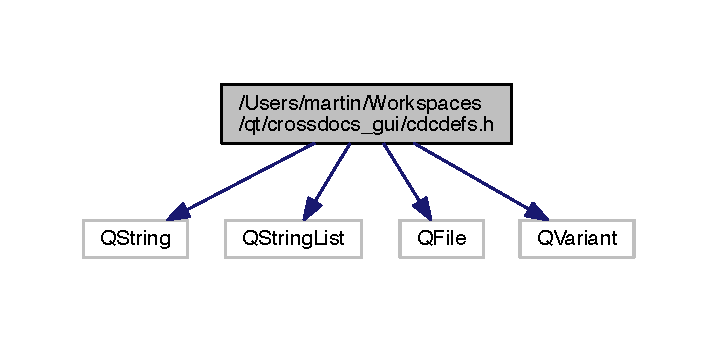
\includegraphics[width=344pt]{cdcdefs_8h__incl}
\end{center}
\end{figure}
This graph shows which files directly or indirectly include this file\+:\nopagebreak
\begin{figure}[H]
\begin{center}
\leavevmode
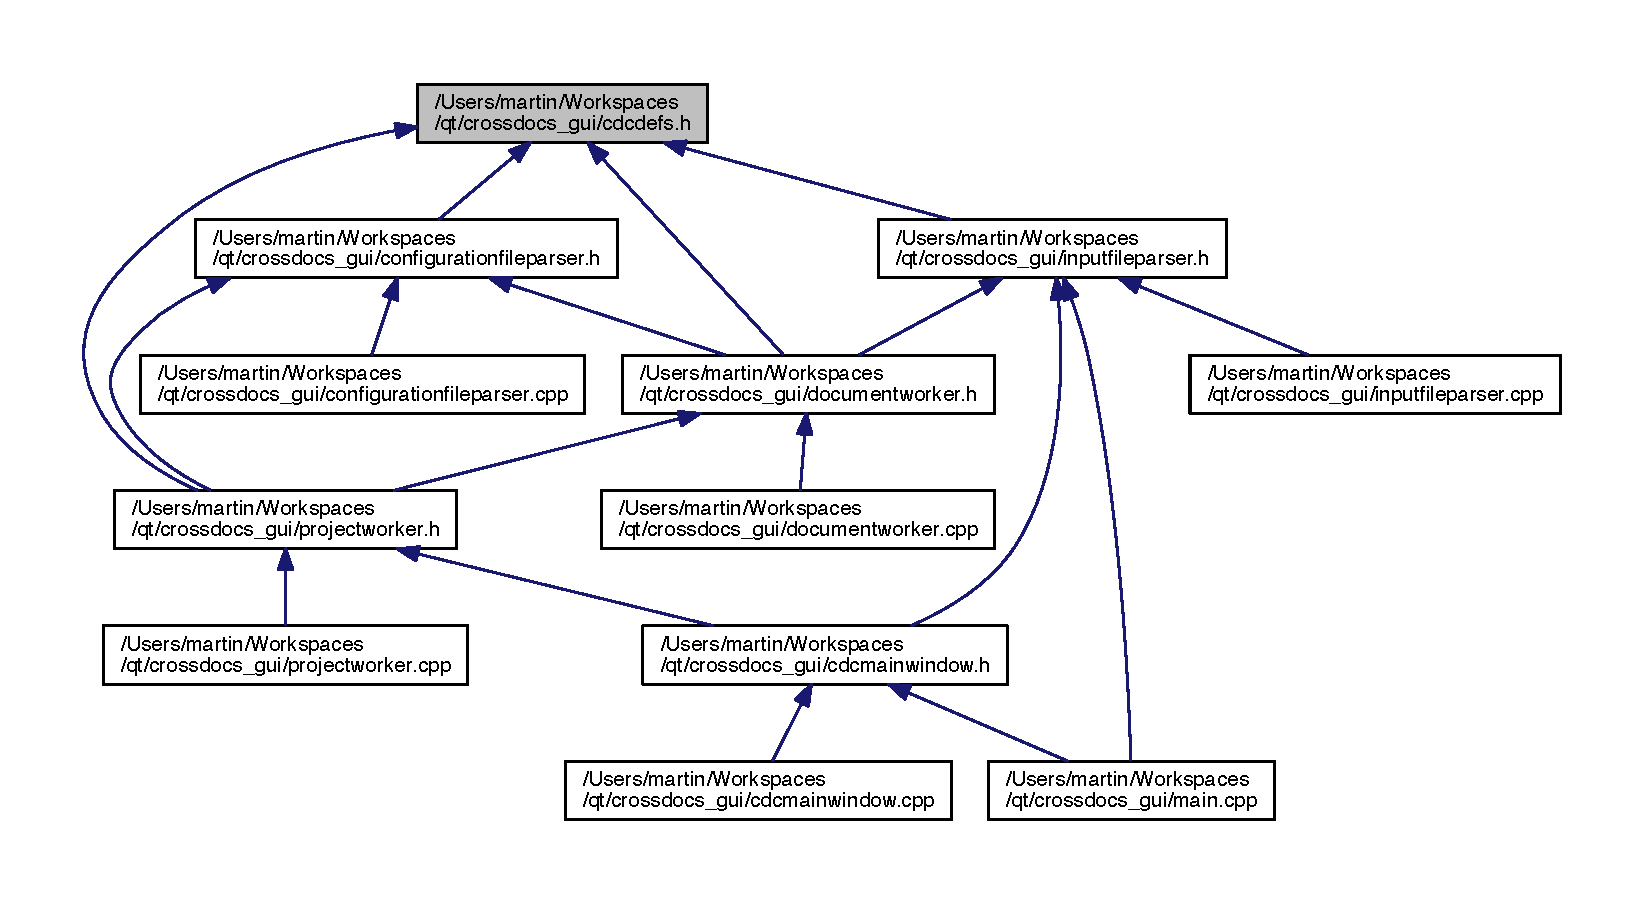
\includegraphics[width=350pt]{cdcdefs_8h__dep__incl}
\end{center}
\end{figure}
\subsection*{Classes}
\begin{DoxyCompactItemize}
\item 
struct \hyperlink{struct_c_d_c__conf_section}{C\+D\+C\+\_\+conf\+Section}
\begin{DoxyCompactList}\small\item\em Structure that contains the header and the contents on each section of a configuration file. \end{DoxyCompactList}\item 
struct \hyperlink{struct_c_d_c__document}{C\+D\+C\+\_\+document}
\begin{DoxyCompactList}\small\item\em Struct that defines one document's parameters. Each document generates independent. \end{DoxyCompactList}\item 
struct \hyperlink{struct_c_d_c__doc_structural_element}{C\+D\+C\+\_\+doc\+Structural\+Element}
\begin{DoxyCompactList}\small\item\em Retains data on the structural sections found in a document's content. \end{DoxyCompactList}\end{DoxyCompactItemize}
\subsection*{Macros}
\begin{DoxyCompactItemize}
\item 
\#define \hyperlink{cdcdefs_8h_a5319875240e8b9b15d9102bf004ba17c}{C\+D\+C\+\_\+\+C\+O\+N\+F\+\_\+\+C\+O\+M\+M\+E\+N\+T}~'\#'
\item 
\#define \hyperlink{cdcdefs_8h_aa6ab19268f451f221daab3ad6d8a682d}{C\+D\+C\+\_\+\+C\+O\+N\+F\+\_\+\+C\+O\+M\+M\+A\+N\+D}~'\+:'
\end{DoxyCompactItemize}
\subsection*{Typedefs}
\begin{DoxyCompactItemize}
\item 
typedef Q\+List$<$ \hyperlink{struct_c_d_c__conf_section}{C\+D\+C\+\_\+conf\+Section} $>$ \hyperlink{cdcdefs_8h_adfd872d2c7ac9d9182576c76af28ea98}{C\+D\+C\+\_\+conf\+List}
\begin{DoxyCompactList}\small\item\em A list of configuration sections. \end{DoxyCompactList}\end{DoxyCompactItemize}
\subsection*{Enumerations}
\begin{DoxyCompactItemize}
\item 
enum \hyperlink{cdcdefs_8h_a7a1ca742b5a041762c1b5784532bd7fd}{C\+D\+C\+\_\+status} \{ \hyperlink{cdcdefs_8h_a7a1ca742b5a041762c1b5784532bd7fda444bcb3a3fcf8389296c49467f27e1d6}{C\+D\+C\+\_\+status\+::ok}, 
\hyperlink{cdcdefs_8h_a7a1ca742b5a041762c1b5784532bd7fda4b4c3d08948825f5fe6b51a1087d503e}{C\+D\+C\+\_\+status\+::io\+Error}, 
\hyperlink{cdcdefs_8h_a7a1ca742b5a041762c1b5784532bd7fda4ce4bdb863d80653ca5b8ad2831c194a}{C\+D\+C\+\_\+status\+::syntax\+Error}, 
\hyperlink{cdcdefs_8h_a7a1ca742b5a041762c1b5784532bd7fda5d748d6271889c2a5fd663d379854752}{C\+D\+C\+\_\+status\+::param\+Error}
 \}
\begin{DoxyCompactList}\small\item\em Enumeration for possible return status on C\+D\+C's methods. \end{DoxyCompactList}\item 
enum \hyperlink{cdcdefs_8h_abd38cc943467f0d66216a60454d5ee06}{C\+D\+C\+\_\+build\+Engine} \{ \hyperlink{cdcdefs_8h_abd38cc943467f0d66216a60454d5ee06a1259e5bf3dfd3ef0991fa65ceeda6fec}{C\+D\+C\+\_\+build\+Engine\+::doxygen}, 
\hyperlink{cdcdefs_8h_abd38cc943467f0d66216a60454d5ee06a590fc197fe73db0aa2ec03687a372eea}{C\+D\+C\+\_\+build\+Engine\+::markdown}, 
\hyperlink{cdcdefs_8h_abd38cc943467f0d66216a60454d5ee06a8b9035807842a4e4dbe009f3f1478127}{C\+D\+C\+\_\+build\+Engine\+::custom}, 
\hyperlink{cdcdefs_8h_abd38cc943467f0d66216a60454d5ee06a334c4a4c42fdb79d7ebc3e73b517e6f8}{C\+D\+C\+\_\+build\+Engine\+::none}
 \}
\begin{DoxyCompactList}\small\item\em For furhter versions -\/ will allow different doc build setups. \end{DoxyCompactList}\item 
enum \hyperlink{cdcdefs_8h_ab649dd84a9663b16384131638df4d313}{C\+D\+C\+\_\+file\+Syntax} \{ \\*
\hyperlink{cdcdefs_8h_ab649dd84a9663b16384131638df4d313a1259e5bf3dfd3ef0991fa65ceeda6fec}{C\+D\+C\+\_\+file\+Syntax\+::doxygen}, 
\hyperlink{cdcdefs_8h_ab649dd84a9663b16384131638df4d313a25f7e525b5c0641e1eb1fb3bdbeb15b5}{C\+D\+C\+\_\+file\+Syntax\+::latex}, 
\hyperlink{cdcdefs_8h_ab649dd84a9663b16384131638df4d313afc35fdc70d5fc69d269883a822c7a53e}{C\+D\+C\+\_\+file\+Syntax\+::html}, 
\hyperlink{cdcdefs_8h_ab649dd84a9663b16384131638df4d313a590fc197fe73db0aa2ec03687a372eea}{C\+D\+C\+\_\+file\+Syntax\+::markdown}, 
\\*
\hyperlink{cdcdefs_8h_ab649dd84a9663b16384131638df4d313a334c4a4c42fdb79d7ebc3e73b517e6f8}{C\+D\+C\+\_\+file\+Syntax\+::none}
 \}
\begin{DoxyCompactList}\small\item\em Defines which syntatical analysis will be performed on a input file. \end{DoxyCompactList}\item 
enum \hyperlink{cdcdefs_8h_a6116ba1886594c273c61d425c61d6416}{C\+D\+C\+\_\+doc\+Structural\+Element\+Type} \{ \hyperlink{cdcdefs_8h_a6116ba1886594c273c61d425c61d6416a73d5342eba070f636ac3246f319bf77f}{C\+D\+C\+\_\+doc\+Structural\+Element\+Type\+::section}, 
\hyperlink{cdcdefs_8h_a6116ba1886594c273c61d425c61d6416a1fa651846210bac7a80f4a684ddd0637}{C\+D\+C\+\_\+doc\+Structural\+Element\+Type\+::subsection}, 
\hyperlink{cdcdefs_8h_a6116ba1886594c273c61d425c61d6416a77d2431676d2643b29bcce4cedc64843}{C\+D\+C\+\_\+doc\+Structural\+Element\+Type\+::subsubsection}, 
\hyperlink{cdcdefs_8h_a6116ba1886594c273c61d425c61d6416a32a97fa20c7928bbe37dea5aec0ebdbd}{C\+D\+C\+\_\+doc\+Structural\+Element\+Type\+::paragraph}
 \}
\end{DoxyCompactItemize}


\subsection{Detailed Description}
Classes, namespaces and types for Cross\+Docs. 



 / \+\_\+\+\_\+ \textbackslash{} $\vert$ \+\_\+ \textbackslash{} $\vert$ / \textbackslash{}/\+\_\+ \+\_\+\+\_\+ \+\_\+\+\_\+\+\_\+ \+\_\+\+\_\+\+\_\+ \+\_\+\+\_\+\+\_\+$\vert$ $\vert$ $\vert$ $\vert$\+\_\+\+\_\+\+\_\+ \+\_\+\+\_\+\+\_\+ \+\_\+\+\_\+\+\_\+ $\vert$ $\vert$ $\vert$ '\+\_\+\+\_\+/ \+\_\+ \textbackslash{}/ \+\_\+\+\_\+/ \+\_\+\+\_\+$\vert$ $\vert$ $\vert$ / \+\_\+ \textbackslash{} / \+\_\+\+\_\+/ \+\_\+\+\_\+$\vert$ $\vert$ \+\_\+\+\_\+/\textbackslash{} $\vert$ $\vert$ $\vert$\+\_\+$\vert$ \+\_\+\+\_\+ \+\_\+\+\_\+ \textbackslash{} $\vert$/ / $\vert$\+\_\+$\vert$ $\vert$ (\+\_\+\+\_\+\+\_\+\+\_\+ \textbackslash{} \+\_\+\+\_\+\+\_\+\+\_\+/\+\_\+$\vert$ \+\_\+\+\_\+\+\_\+/$\vert$\+\_\+\+\_\+\+\_\+/\+\_\+\+\_\+\+\_\+/\+\_\+\+\_\+\+\_\+/ \+\_\+\+\_\+\+\_\+/ \+\_\+\+\_\+\+\_\+$\vert$\+\_\+\+\_\+\+\_\+/

\begin{DoxyAuthor}{Author}
Martin Vincent Bloedorn 
\end{DoxyAuthor}
\begin{DoxyVersion}{Version}
V0.\+1.\+0 
\end{DoxyVersion}
\begin{DoxyDate}{Date}
15-\/\+August-\/2014 
\end{DoxyDate}


Definition in file \hyperlink{cdcdefs_8h_source}{cdcdefs.\+h}.



\subsection{Macro Definition Documentation}
\hypertarget{cdcdefs_8h_aa6ab19268f451f221daab3ad6d8a682d}{\index{cdcdefs.\+h@{cdcdefs.\+h}!C\+D\+C\+\_\+\+C\+O\+N\+F\+\_\+\+C\+O\+M\+M\+A\+N\+D@{C\+D\+C\+\_\+\+C\+O\+N\+F\+\_\+\+C\+O\+M\+M\+A\+N\+D}}
\index{C\+D\+C\+\_\+\+C\+O\+N\+F\+\_\+\+C\+O\+M\+M\+A\+N\+D@{C\+D\+C\+\_\+\+C\+O\+N\+F\+\_\+\+C\+O\+M\+M\+A\+N\+D}!cdcdefs.\+h@{cdcdefs.\+h}}
\subsubsection[{C\+D\+C\+\_\+\+C\+O\+N\+F\+\_\+\+C\+O\+M\+M\+A\+N\+D}]{\setlength{\rightskip}{0pt plus 5cm}\#define C\+D\+C\+\_\+\+C\+O\+N\+F\+\_\+\+C\+O\+M\+M\+A\+N\+D~'\+:'}}\label{cdcdefs_8h_aa6ab19268f451f221daab3ad6d8a682d}


Definition at line 99 of file cdcdefs.\+h.

\hypertarget{cdcdefs_8h_a5319875240e8b9b15d9102bf004ba17c}{\index{cdcdefs.\+h@{cdcdefs.\+h}!C\+D\+C\+\_\+\+C\+O\+N\+F\+\_\+\+C\+O\+M\+M\+E\+N\+T@{C\+D\+C\+\_\+\+C\+O\+N\+F\+\_\+\+C\+O\+M\+M\+E\+N\+T}}
\index{C\+D\+C\+\_\+\+C\+O\+N\+F\+\_\+\+C\+O\+M\+M\+E\+N\+T@{C\+D\+C\+\_\+\+C\+O\+N\+F\+\_\+\+C\+O\+M\+M\+E\+N\+T}!cdcdefs.\+h@{cdcdefs.\+h}}
\subsubsection[{C\+D\+C\+\_\+\+C\+O\+N\+F\+\_\+\+C\+O\+M\+M\+E\+N\+T}]{\setlength{\rightskip}{0pt plus 5cm}\#define C\+D\+C\+\_\+\+C\+O\+N\+F\+\_\+\+C\+O\+M\+M\+E\+N\+T~'\#'}}\label{cdcdefs_8h_a5319875240e8b9b15d9102bf004ba17c}


Definition at line 98 of file cdcdefs.\+h.



\subsection{Typedef Documentation}
\hypertarget{cdcdefs_8h_adfd872d2c7ac9d9182576c76af28ea98}{\index{cdcdefs.\+h@{cdcdefs.\+h}!C\+D\+C\+\_\+conf\+List@{C\+D\+C\+\_\+conf\+List}}
\index{C\+D\+C\+\_\+conf\+List@{C\+D\+C\+\_\+conf\+List}!cdcdefs.\+h@{cdcdefs.\+h}}
\subsubsection[{C\+D\+C\+\_\+conf\+List}]{\setlength{\rightskip}{0pt plus 5cm}typedef Q\+List$<${\bf C\+D\+C\+\_\+conf\+Section}$>$ {\bf C\+D\+C\+\_\+conf\+List}}}\label{cdcdefs_8h_adfd872d2c7ac9d9182576c76af28ea98}


A list of configuration sections. 

Represents data obtained from a conf file, or data that will be saved to a file. 

Definition at line 54 of file cdcdefs.\+h.



\subsection{Enumeration Type Documentation}
\hypertarget{cdcdefs_8h_abd38cc943467f0d66216a60454d5ee06}{\index{cdcdefs.\+h@{cdcdefs.\+h}!C\+D\+C\+\_\+build\+Engine@{C\+D\+C\+\_\+build\+Engine}}
\index{C\+D\+C\+\_\+build\+Engine@{C\+D\+C\+\_\+build\+Engine}!cdcdefs.\+h@{cdcdefs.\+h}}
\subsubsection[{C\+D\+C\+\_\+build\+Engine}]{\setlength{\rightskip}{0pt plus 5cm}enum {\bf C\+D\+C\+\_\+build\+Engine}\hspace{0.3cm}{\ttfamily [strong]}}}\label{cdcdefs_8h_abd38cc943467f0d66216a60454d5ee06}


For furhter versions -\/ will allow different doc build setups. 

\begin{Desc}
\item[Enumerator]\par
\begin{description}
\index{doxygen@{doxygen}!cdcdefs.\+h@{cdcdefs.\+h}}\index{cdcdefs.\+h@{cdcdefs.\+h}!doxygen@{doxygen}}\item[{\em 
\hypertarget{cdcdefs_8h_abd38cc943467f0d66216a60454d5ee06a1259e5bf3dfd3ef0991fa65ceeda6fec}{doxygen}\label{cdcdefs_8h_abd38cc943467f0d66216a60454d5ee06a1259e5bf3dfd3ef0991fa65ceeda6fec}
}]\index{markdown@{markdown}!cdcdefs.\+h@{cdcdefs.\+h}}\index{cdcdefs.\+h@{cdcdefs.\+h}!markdown@{markdown}}\item[{\em 
\hypertarget{cdcdefs_8h_abd38cc943467f0d66216a60454d5ee06a590fc197fe73db0aa2ec03687a372eea}{markdown}\label{cdcdefs_8h_abd38cc943467f0d66216a60454d5ee06a590fc197fe73db0aa2ec03687a372eea}
}]\index{custom@{custom}!cdcdefs.\+h@{cdcdefs.\+h}}\index{cdcdefs.\+h@{cdcdefs.\+h}!custom@{custom}}\item[{\em 
\hypertarget{cdcdefs_8h_abd38cc943467f0d66216a60454d5ee06a8b9035807842a4e4dbe009f3f1478127}{custom}\label{cdcdefs_8h_abd38cc943467f0d66216a60454d5ee06a8b9035807842a4e4dbe009f3f1478127}
}]\index{none@{none}!cdcdefs.\+h@{cdcdefs.\+h}}\index{cdcdefs.\+h@{cdcdefs.\+h}!none@{none}}\item[{\em 
\hypertarget{cdcdefs_8h_abd38cc943467f0d66216a60454d5ee06a334c4a4c42fdb79d7ebc3e73b517e6f8}{none}\label{cdcdefs_8h_abd38cc943467f0d66216a60454d5ee06a334c4a4c42fdb79d7ebc3e73b517e6f8}
}]When no build engine is specified, the conf. next hierarchically available option. \end{description}
\end{Desc}


Definition at line 57 of file cdcdefs.\+h.

\hypertarget{cdcdefs_8h_a6116ba1886594c273c61d425c61d6416}{\index{cdcdefs.\+h@{cdcdefs.\+h}!C\+D\+C\+\_\+doc\+Structural\+Element\+Type@{C\+D\+C\+\_\+doc\+Structural\+Element\+Type}}
\index{C\+D\+C\+\_\+doc\+Structural\+Element\+Type@{C\+D\+C\+\_\+doc\+Structural\+Element\+Type}!cdcdefs.\+h@{cdcdefs.\+h}}
\subsubsection[{C\+D\+C\+\_\+doc\+Structural\+Element\+Type}]{\setlength{\rightskip}{0pt plus 5cm}enum {\bf C\+D\+C\+\_\+doc\+Structural\+Element\+Type}\hspace{0.3cm}{\ttfamily [strong]}}}\label{cdcdefs_8h_a6116ba1886594c273c61d425c61d6416}
\begin{Desc}
\item[Enumerator]\par
\begin{description}
\index{section@{section}!cdcdefs.\+h@{cdcdefs.\+h}}\index{cdcdefs.\+h@{cdcdefs.\+h}!section@{section}}\item[{\em 
\hypertarget{cdcdefs_8h_a6116ba1886594c273c61d425c61d6416a73d5342eba070f636ac3246f319bf77f}{section}\label{cdcdefs_8h_a6116ba1886594c273c61d425c61d6416a73d5342eba070f636ac3246f319bf77f}
}]\index{subsection@{subsection}!cdcdefs.\+h@{cdcdefs.\+h}}\index{cdcdefs.\+h@{cdcdefs.\+h}!subsection@{subsection}}\item[{\em 
\hypertarget{cdcdefs_8h_a6116ba1886594c273c61d425c61d6416a1fa651846210bac7a80f4a684ddd0637}{subsection}\label{cdcdefs_8h_a6116ba1886594c273c61d425c61d6416a1fa651846210bac7a80f4a684ddd0637}
}]\index{subsubsection@{subsubsection}!cdcdefs.\+h@{cdcdefs.\+h}}\index{cdcdefs.\+h@{cdcdefs.\+h}!subsubsection@{subsubsection}}\item[{\em 
\hypertarget{cdcdefs_8h_a6116ba1886594c273c61d425c61d6416a77d2431676d2643b29bcce4cedc64843}{subsubsection}\label{cdcdefs_8h_a6116ba1886594c273c61d425c61d6416a77d2431676d2643b29bcce4cedc64843}
}]\index{paragraph@{paragraph}!cdcdefs.\+h@{cdcdefs.\+h}}\index{cdcdefs.\+h@{cdcdefs.\+h}!paragraph@{paragraph}}\item[{\em 
\hypertarget{cdcdefs_8h_a6116ba1886594c273c61d425c61d6416a32a97fa20c7928bbe37dea5aec0ebdbd}{paragraph}\label{cdcdefs_8h_a6116ba1886594c273c61d425c61d6416a32a97fa20c7928bbe37dea5aec0ebdbd}
}]\end{description}
\end{Desc}


Definition at line 73 of file cdcdefs.\+h.

\hypertarget{cdcdefs_8h_ab649dd84a9663b16384131638df4d313}{\index{cdcdefs.\+h@{cdcdefs.\+h}!C\+D\+C\+\_\+file\+Syntax@{C\+D\+C\+\_\+file\+Syntax}}
\index{C\+D\+C\+\_\+file\+Syntax@{C\+D\+C\+\_\+file\+Syntax}!cdcdefs.\+h@{cdcdefs.\+h}}
\subsubsection[{C\+D\+C\+\_\+file\+Syntax}]{\setlength{\rightskip}{0pt plus 5cm}enum {\bf C\+D\+C\+\_\+file\+Syntax}\hspace{0.3cm}{\ttfamily [strong]}}}\label{cdcdefs_8h_ab649dd84a9663b16384131638df4d313}


Defines which syntatical analysis will be performed on a input file. 

\begin{Desc}
\item[Enumerator]\par
\begin{description}
\index{doxygen@{doxygen}!cdcdefs.\+h@{cdcdefs.\+h}}\index{cdcdefs.\+h@{cdcdefs.\+h}!doxygen@{doxygen}}\item[{\em 
\hypertarget{cdcdefs_8h_ab649dd84a9663b16384131638df4d313a1259e5bf3dfd3ef0991fa65ceeda6fec}{doxygen}\label{cdcdefs_8h_ab649dd84a9663b16384131638df4d313a1259e5bf3dfd3ef0991fa65ceeda6fec}
}]\index{latex@{latex}!cdcdefs.\+h@{cdcdefs.\+h}}\index{cdcdefs.\+h@{cdcdefs.\+h}!latex@{latex}}\item[{\em 
\hypertarget{cdcdefs_8h_ab649dd84a9663b16384131638df4d313a25f7e525b5c0641e1eb1fb3bdbeb15b5}{latex}\label{cdcdefs_8h_ab649dd84a9663b16384131638df4d313a25f7e525b5c0641e1eb1fb3bdbeb15b5}
}]\index{html@{html}!cdcdefs.\+h@{cdcdefs.\+h}}\index{cdcdefs.\+h@{cdcdefs.\+h}!html@{html}}\item[{\em 
\hypertarget{cdcdefs_8h_ab649dd84a9663b16384131638df4d313afc35fdc70d5fc69d269883a822c7a53e}{html}\label{cdcdefs_8h_ab649dd84a9663b16384131638df4d313afc35fdc70d5fc69d269883a822c7a53e}
}]\index{markdown@{markdown}!cdcdefs.\+h@{cdcdefs.\+h}}\index{cdcdefs.\+h@{cdcdefs.\+h}!markdown@{markdown}}\item[{\em 
\hypertarget{cdcdefs_8h_ab649dd84a9663b16384131638df4d313a590fc197fe73db0aa2ec03687a372eea}{markdown}\label{cdcdefs_8h_ab649dd84a9663b16384131638df4d313a590fc197fe73db0aa2ec03687a372eea}
}]\index{none@{none}!cdcdefs.\+h@{cdcdefs.\+h}}\index{cdcdefs.\+h@{cdcdefs.\+h}!none@{none}}\item[{\em 
\hypertarget{cdcdefs_8h_ab649dd84a9663b16384131638df4d313a334c4a4c42fdb79d7ebc3e73b517e6f8}{none}\label{cdcdefs_8h_ab649dd84a9663b16384131638df4d313a334c4a4c42fdb79d7ebc3e73b517e6f8}
}]\end{description}
\end{Desc}


Definition at line 65 of file cdcdefs.\+h.

\hypertarget{cdcdefs_8h_a7a1ca742b5a041762c1b5784532bd7fd}{\index{cdcdefs.\+h@{cdcdefs.\+h}!C\+D\+C\+\_\+status@{C\+D\+C\+\_\+status}}
\index{C\+D\+C\+\_\+status@{C\+D\+C\+\_\+status}!cdcdefs.\+h@{cdcdefs.\+h}}
\subsubsection[{C\+D\+C\+\_\+status}]{\setlength{\rightskip}{0pt plus 5cm}enum {\bf C\+D\+C\+\_\+status}\hspace{0.3cm}{\ttfamily [strong]}}}\label{cdcdefs_8h_a7a1ca742b5a041762c1b5784532bd7fd}


Enumeration for possible return status on C\+D\+C's methods. 

\begin{DoxyRefDesc}{Todo}
\item[\hyperlink{todo__todo000001}{Todo}]Document each status (they are, as of this version, not yet fully defined). \end{DoxyRefDesc}
\begin{Desc}
\item[Enumerator]\par
\begin{description}
\index{ok@{ok}!cdcdefs.\+h@{cdcdefs.\+h}}\index{cdcdefs.\+h@{cdcdefs.\+h}!ok@{ok}}\item[{\em 
\hypertarget{cdcdefs_8h_a7a1ca742b5a041762c1b5784532bd7fda444bcb3a3fcf8389296c49467f27e1d6}{ok}\label{cdcdefs_8h_a7a1ca742b5a041762c1b5784532bd7fda444bcb3a3fcf8389296c49467f27e1d6}
}]\index{io\+Error@{io\+Error}!cdcdefs.\+h@{cdcdefs.\+h}}\index{cdcdefs.\+h@{cdcdefs.\+h}!io\+Error@{io\+Error}}\item[{\em 
\hypertarget{cdcdefs_8h_a7a1ca742b5a041762c1b5784532bd7fda4b4c3d08948825f5fe6b51a1087d503e}{io\+Error}\label{cdcdefs_8h_a7a1ca742b5a041762c1b5784532bd7fda4b4c3d08948825f5fe6b51a1087d503e}
}]Operation went ok. \index{syntax\+Error@{syntax\+Error}!cdcdefs.\+h@{cdcdefs.\+h}}\index{cdcdefs.\+h@{cdcdefs.\+h}!syntax\+Error@{syntax\+Error}}\item[{\em 
\hypertarget{cdcdefs_8h_a7a1ca742b5a041762c1b5784532bd7fda4ce4bdb863d80653ca5b8ad2831c194a}{syntax\+Error}\label{cdcdefs_8h_a7a1ca742b5a041762c1b5784532bd7fda4ce4bdb863d80653ca5b8ad2831c194a}
}]Operation failed due to I\+O error (file-\/related) \index{param\+Error@{param\+Error}!cdcdefs.\+h@{cdcdefs.\+h}}\index{cdcdefs.\+h@{cdcdefs.\+h}!param\+Error@{param\+Error}}\item[{\em 
\hypertarget{cdcdefs_8h_a7a1ca742b5a041762c1b5784532bd7fda5d748d6271889c2a5fd663d379854752}{param\+Error}\label{cdcdefs_8h_a7a1ca742b5a041762c1b5784532bd7fda5d748d6271889c2a5fd663d379854752}
}]Operation failed due to syntax error in a file. Invalid parameter passed to method \end{description}
\end{Desc}


Definition at line 34 of file cdcdefs.\+h.


\hypertarget{cdcmainwindow_8cpp}{\section{/\+Users/martin/\+Workspaces/qt/crossdocs\+\_\+gui/cdcmainwindow.cpp File Reference}
\label{cdcmainwindow_8cpp}\index{/\+Users/martin/\+Workspaces/qt/crossdocs\+\_\+gui/cdcmainwindow.\+cpp@{/\+Users/martin/\+Workspaces/qt/crossdocs\+\_\+gui/cdcmainwindow.\+cpp}}
}
{\ttfamily \#include \char`\"{}cdcmainwindow.\+h\char`\"{}}\\*
{\ttfamily \#include $<$iostream$>$}\\*
Include dependency graph for cdcmainwindow.\+cpp\+:\nopagebreak
\begin{figure}[H]
\begin{center}
\leavevmode
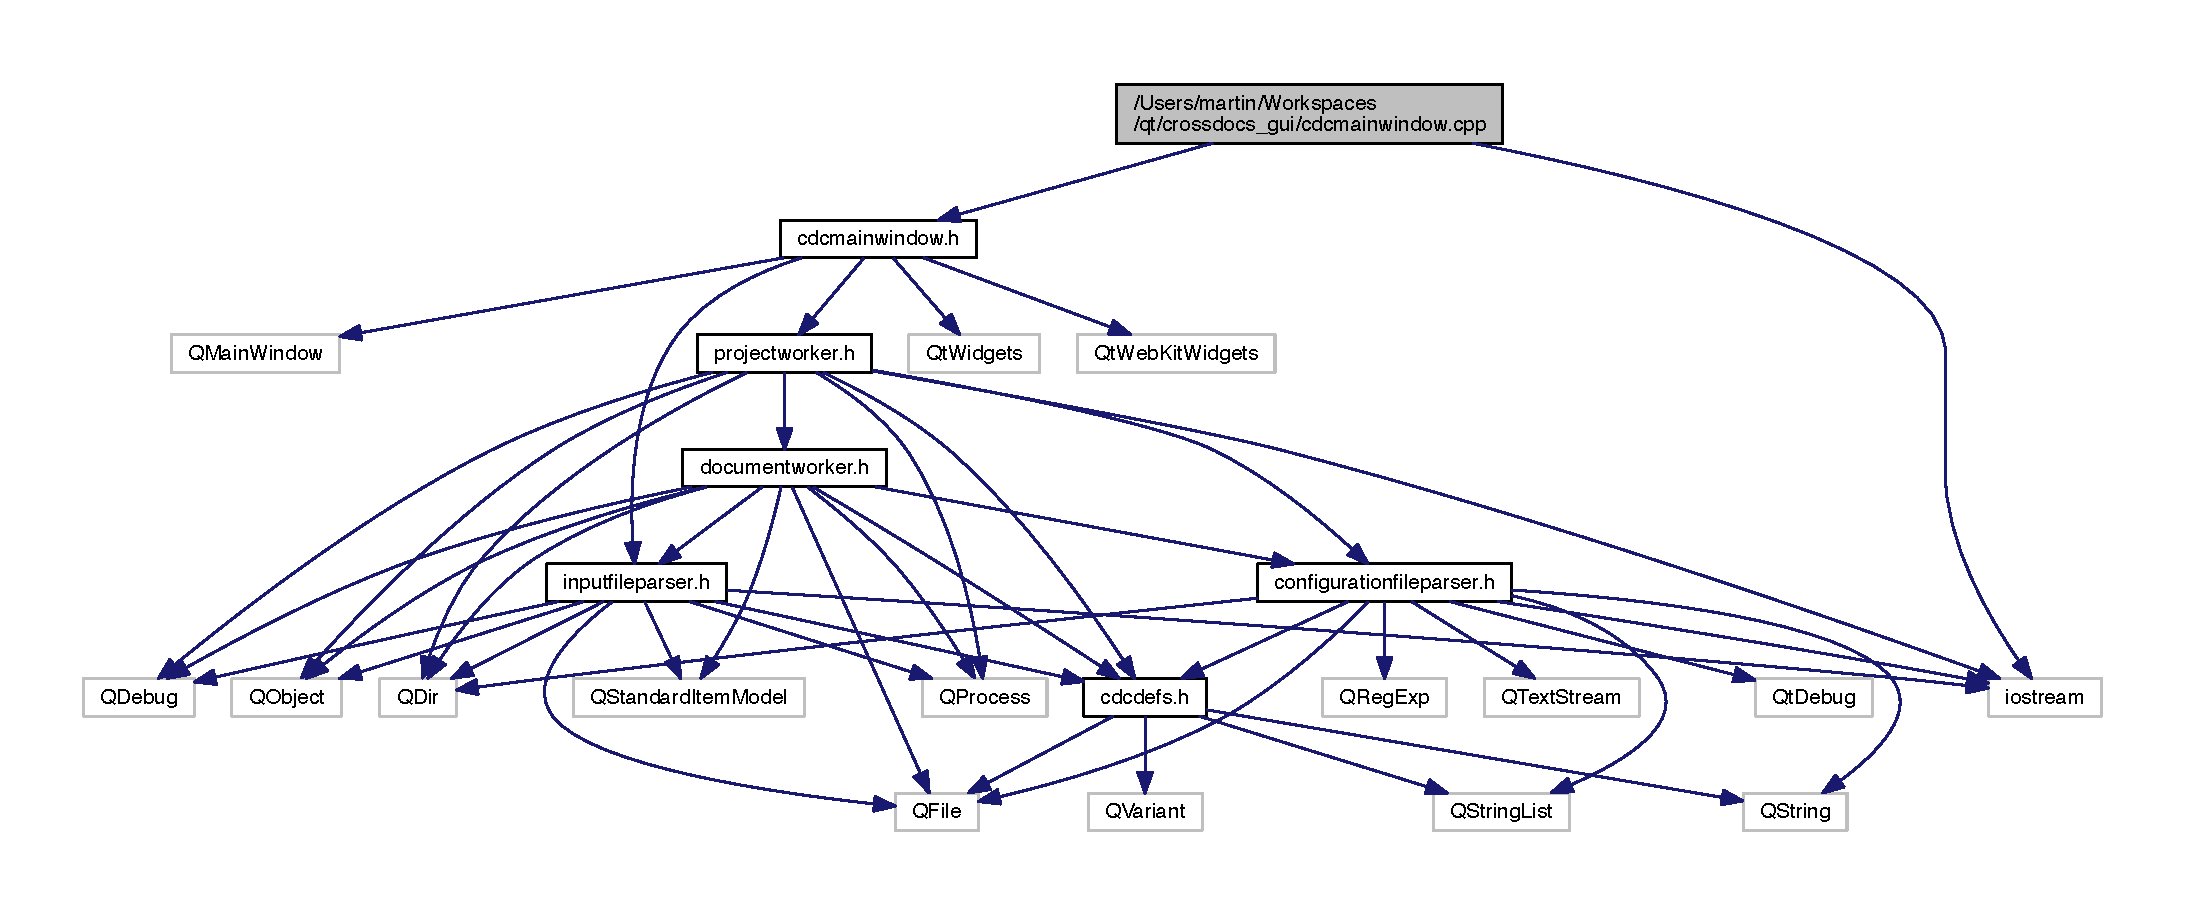
\includegraphics[width=350pt]{cdcmainwindow_8cpp__incl}
\end{center}
\end{figure}

\hypertarget{cdcmainwindow_8h}{\section{/\+Users/martin/\+Workspaces/qt/crossdocs\+\_\+gui/cdcmainwindow.h File Reference}
\label{cdcmainwindow_8h}\index{/\+Users/martin/\+Workspaces/qt/crossdocs\+\_\+gui/cdcmainwindow.\+h@{/\+Users/martin/\+Workspaces/qt/crossdocs\+\_\+gui/cdcmainwindow.\+h}}
}
{\ttfamily \#include $<$Q\+Main\+Window$>$}\\*
{\ttfamily \#include $<$Qt\+Widgets$>$}\\*
{\ttfamily \#include $<$Qt\+Web\+Kit\+Widgets$>$}\\*
{\ttfamily \#include \char`\"{}projectworker.\+h\char`\"{}}\\*
{\ttfamily \#include \char`\"{}inputfileparser.\+h\char`\"{}}\\*
Include dependency graph for cdcmainwindow.\+h\+:\nopagebreak
\begin{figure}[H]
\begin{center}
\leavevmode
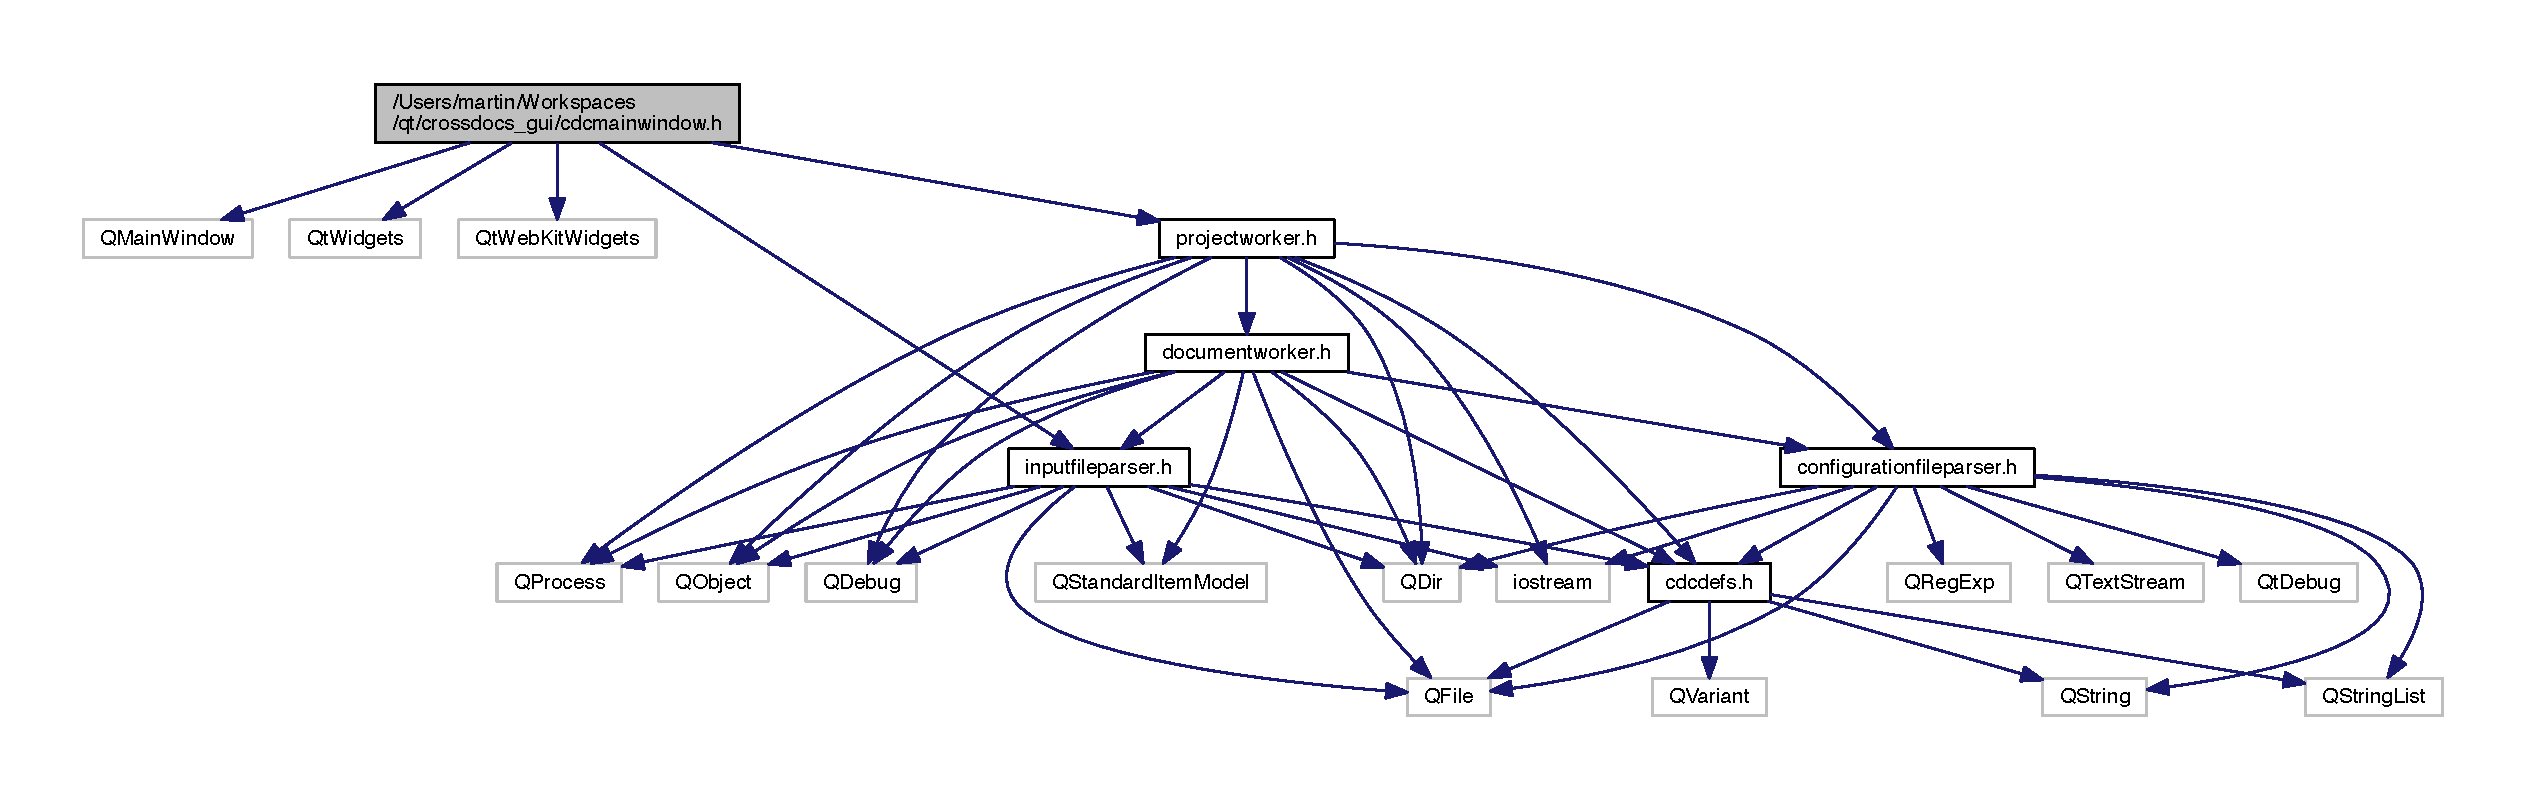
\includegraphics[width=350pt]{cdcmainwindow_8h__incl}
\end{center}
\end{figure}
This graph shows which files directly or indirectly include this file\+:\nopagebreak
\begin{figure}[H]
\begin{center}
\leavevmode
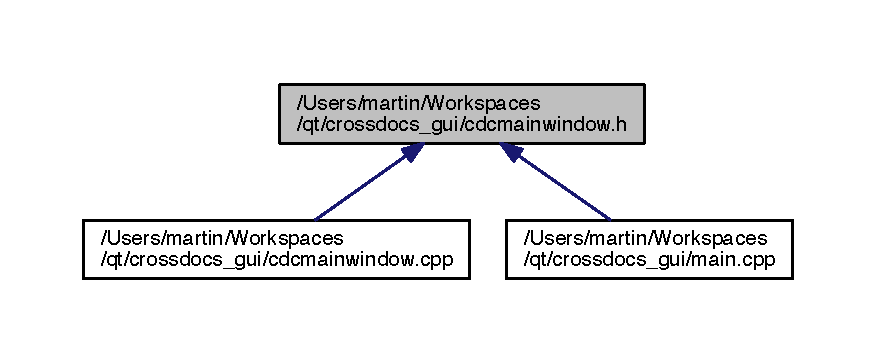
\includegraphics[width=350pt]{cdcmainwindow_8h__dep__incl}
\end{center}
\end{figure}
\subsection*{Classes}
\begin{DoxyCompactItemize}
\item 
class \hyperlink{classcdc_main_window}{cdc\+Main\+Window}
\end{DoxyCompactItemize}

\hypertarget{configurationfileparser_8cpp}{\section{/\+Users/martin/\+Workspaces/qt/crossdocs\+\_\+gui/configurationfileparser.cpp File Reference}
\label{configurationfileparser_8cpp}\index{/\+Users/martin/\+Workspaces/qt/crossdocs\+\_\+gui/configurationfileparser.\+cpp@{/\+Users/martin/\+Workspaces/qt/crossdocs\+\_\+gui/configurationfileparser.\+cpp}}
}


Definitions for $\ast$.cdc file parsing.  


{\ttfamily \#include \char`\"{}configurationfileparser.\+h\char`\"{}}\\*
Include dependency graph for configurationfileparser.\+cpp\+:\nopagebreak
\begin{figure}[H]
\begin{center}
\leavevmode
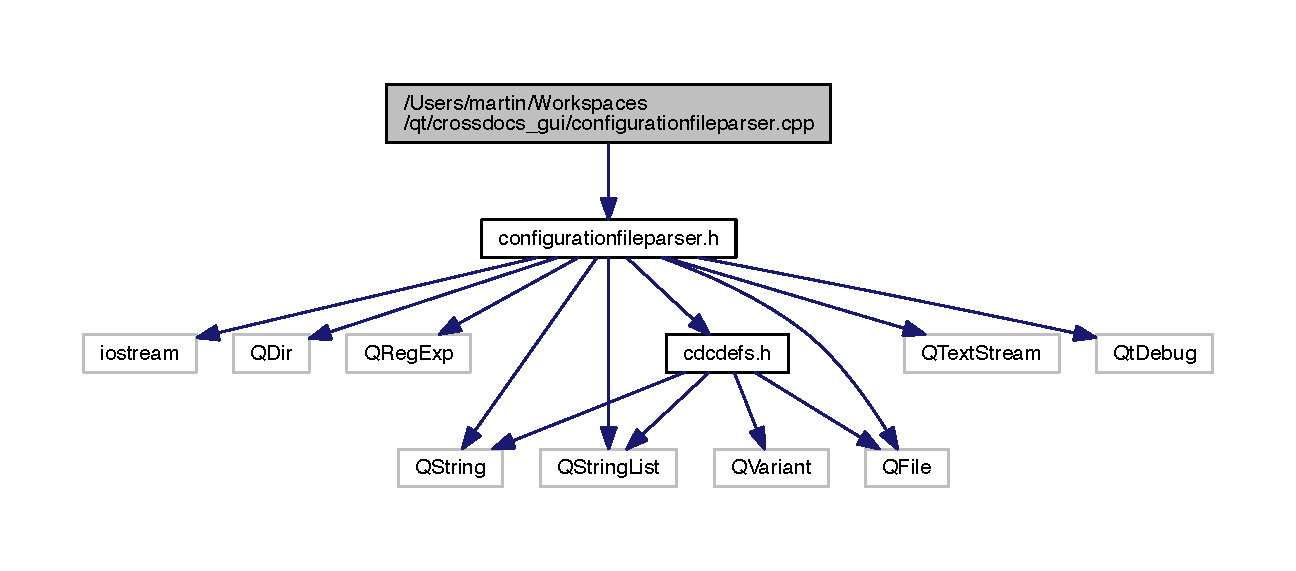
\includegraphics[width=350pt]{configurationfileparser_8cpp__incl}
\end{center}
\end{figure}
\subsection*{Enumerations}
\begin{DoxyCompactItemize}
\item 
enum \hyperlink{configurationfileparser_8cpp_a03975fe93d45f171264b2ac18fdd47cb}{C\+D\+C\+\_\+c\+State} \{ \hyperlink{configurationfileparser_8cpp_a03975fe93d45f171264b2ac18fdd47cbaec2f993aec2c27fc750119ab17b16cdb}{C\+D\+C\+\_\+c\+State\+::idle}, 
\hyperlink{configurationfileparser_8cpp_a03975fe93d45f171264b2ac18fdd47cba8ff8a0434cd2480bbba581a4e93b78f3}{C\+D\+C\+\_\+c\+State\+::at\+\_\+header}, 
\hyperlink{configurationfileparser_8cpp_a03975fe93d45f171264b2ac18fdd47cbad9eec784bf1f493012bcbcde06f3e4b9}{C\+D\+C\+\_\+c\+State\+::at\+\_\+argument}, 
\hyperlink{configurationfileparser_8cpp_a03975fe93d45f171264b2ac18fdd47cbae11185b6e35c1b767174dc988aa0f179}{C\+D\+C\+\_\+c\+State\+::fail}
 \}
\end{DoxyCompactItemize}


\subsection{Detailed Description}
Definitions for $\ast$.cdc file parsing. 



 / \+\_\+\+\_\+ \textbackslash{} $\vert$ \+\_\+ \textbackslash{} $\vert$ / \textbackslash{}/\+\_\+ \+\_\+\+\_\+ \+\_\+\+\_\+\+\_\+ \+\_\+\+\_\+\+\_\+ \+\_\+\+\_\+\+\_\+$\vert$ $\vert$ $\vert$ $\vert$\+\_\+\+\_\+\+\_\+ \+\_\+\+\_\+\+\_\+ \+\_\+\+\_\+\+\_\+ $\vert$ $\vert$ $\vert$ '\+\_\+\+\_\+/ \+\_\+ \textbackslash{}/ \+\_\+\+\_\+/ \+\_\+\+\_\+$\vert$ $\vert$ $\vert$ / \+\_\+ \textbackslash{} / \+\_\+\+\_\+/ \+\_\+\+\_\+$\vert$ $\vert$ \+\_\+\+\_\+/\textbackslash{} $\vert$ $\vert$ $\vert$\+\_\+$\vert$ \+\_\+\+\_\+ \+\_\+\+\_\+ \textbackslash{} $\vert$/ / $\vert$\+\_\+$\vert$ $\vert$ (\+\_\+\+\_\+\+\_\+\+\_\+ \textbackslash{} \+\_\+\+\_\+\+\_\+\+\_\+/\+\_\+$\vert$ \+\_\+\+\_\+\+\_\+/$\vert$\+\_\+\+\_\+\+\_\+/\+\_\+\+\_\+\+\_\+/\+\_\+\+\_\+\+\_\+/ \+\_\+\+\_\+\+\_\+/ \+\_\+\+\_\+\+\_\+$\vert$\+\_\+\+\_\+\+\_\+/

\begin{DoxyAuthor}{Author}
Martin Vincent Bloedorn 
\end{DoxyAuthor}
\begin{DoxyVersion}{Version}
V0.\+1.\+0 
\end{DoxyVersion}
\begin{DoxyDate}{Date}
03-\/\+August-\/2014 
\end{DoxyDate}


Definition in file \hyperlink{configurationfileparser_8cpp_source}{configurationfileparser.\+cpp}.



\subsection{Enumeration Type Documentation}
\hypertarget{configurationfileparser_8cpp_a03975fe93d45f171264b2ac18fdd47cb}{\index{configurationfileparser.\+cpp@{configurationfileparser.\+cpp}!C\+D\+C\+\_\+c\+State@{C\+D\+C\+\_\+c\+State}}
\index{C\+D\+C\+\_\+c\+State@{C\+D\+C\+\_\+c\+State}!configurationfileparser.\+cpp@{configurationfileparser.\+cpp}}
\subsubsection[{C\+D\+C\+\_\+c\+State}]{\setlength{\rightskip}{0pt plus 5cm}enum {\bf C\+D\+C\+\_\+c\+State}\hspace{0.3cm}{\ttfamily [strong]}}}\label{configurationfileparser_8cpp_a03975fe93d45f171264b2ac18fdd47cb}
\begin{Desc}
\item[Enumerator]\par
\begin{description}
\index{idle@{idle}!configurationfileparser.\+cpp@{configurationfileparser.\+cpp}}\index{configurationfileparser.\+cpp@{configurationfileparser.\+cpp}!idle@{idle}}\item[{\em 
\hypertarget{configurationfileparser_8cpp_a03975fe93d45f171264b2ac18fdd47cbaec2f993aec2c27fc750119ab17b16cdb}{idle}\label{configurationfileparser_8cpp_a03975fe93d45f171264b2ac18fdd47cbaec2f993aec2c27fc750119ab17b16cdb}
}]\index{at\+\_\+header@{at\+\_\+header}!configurationfileparser.\+cpp@{configurationfileparser.\+cpp}}\index{configurationfileparser.\+cpp@{configurationfileparser.\+cpp}!at\+\_\+header@{at\+\_\+header}}\item[{\em 
\hypertarget{configurationfileparser_8cpp_a03975fe93d45f171264b2ac18fdd47cba8ff8a0434cd2480bbba581a4e93b78f3}{at\+\_\+header}\label{configurationfileparser_8cpp_a03975fe93d45f171264b2ac18fdd47cba8ff8a0434cd2480bbba581a4e93b78f3}
}]\index{at\+\_\+argument@{at\+\_\+argument}!configurationfileparser.\+cpp@{configurationfileparser.\+cpp}}\index{configurationfileparser.\+cpp@{configurationfileparser.\+cpp}!at\+\_\+argument@{at\+\_\+argument}}\item[{\em 
\hypertarget{configurationfileparser_8cpp_a03975fe93d45f171264b2ac18fdd47cbad9eec784bf1f493012bcbcde06f3e4b9}{at\+\_\+argument}\label{configurationfileparser_8cpp_a03975fe93d45f171264b2ac18fdd47cbad9eec784bf1f493012bcbcde06f3e4b9}
}]\index{fail@{fail}!configurationfileparser.\+cpp@{configurationfileparser.\+cpp}}\index{configurationfileparser.\+cpp@{configurationfileparser.\+cpp}!fail@{fail}}\item[{\em 
\hypertarget{configurationfileparser_8cpp_a03975fe93d45f171264b2ac18fdd47cbae11185b6e35c1b767174dc988aa0f179}{fail}\label{configurationfileparser_8cpp_a03975fe93d45f171264b2ac18fdd47cbae11185b6e35c1b767174dc988aa0f179}
}]\end{description}
\end{Desc}


Definition at line 23 of file configurationfileparser.\+cpp.


\hypertarget{configurationfileparser_8h}{\section{/\+Users/martin/\+Workspaces/qt/crossdocs\+\_\+gui/configurationfileparser.h File Reference}
\label{configurationfileparser_8h}\index{/\+Users/martin/\+Workspaces/qt/crossdocs\+\_\+gui/configurationfileparser.\+h@{/\+Users/martin/\+Workspaces/qt/crossdocs\+\_\+gui/configurationfileparser.\+h}}
}


Definitions for $\ast$.cdc file parsing.  


{\ttfamily \#include $<$iostream$>$}\\*
{\ttfamily \#include $<$Q\+Dir$>$}\\*
{\ttfamily \#include $<$Q\+Reg\+Exp$>$}\\*
{\ttfamily \#include $<$Q\+String$>$}\\*
{\ttfamily \#include $<$Q\+String\+List$>$}\\*
{\ttfamily \#include $<$Q\+File$>$}\\*
{\ttfamily \#include $<$Q\+Text\+Stream$>$}\\*
{\ttfamily \#include $<$Qt\+Debug$>$}\\*
{\ttfamily \#include \char`\"{}cdcdefs.\+h\char`\"{}}\\*
Include dependency graph for configurationfileparser.\+h\+:\nopagebreak
\begin{figure}[H]
\begin{center}
\leavevmode
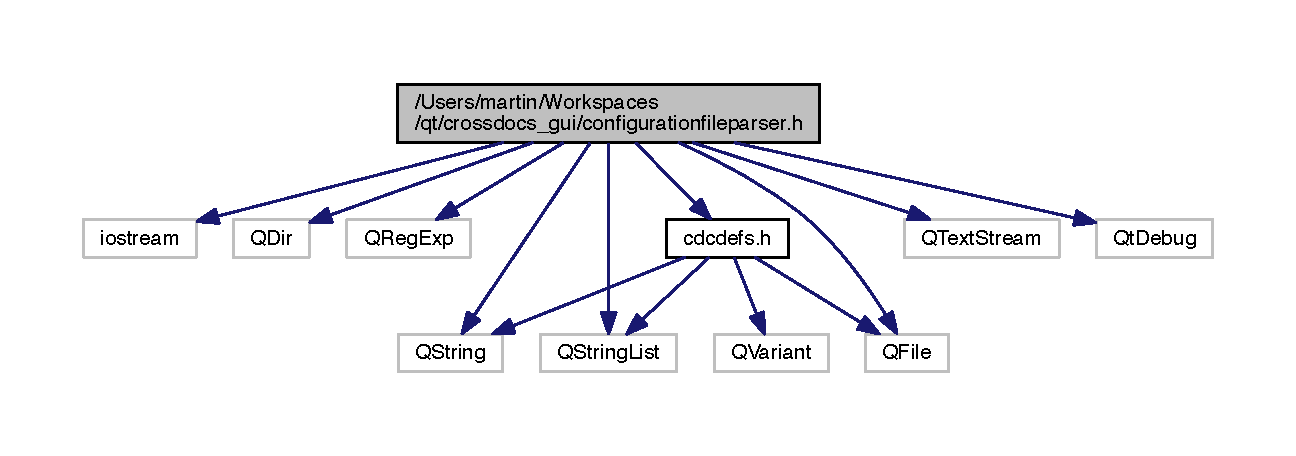
\includegraphics[width=350pt]{configurationfileparser_8h__incl}
\end{center}
\end{figure}
This graph shows which files directly or indirectly include this file\+:\nopagebreak
\begin{figure}[H]
\begin{center}
\leavevmode
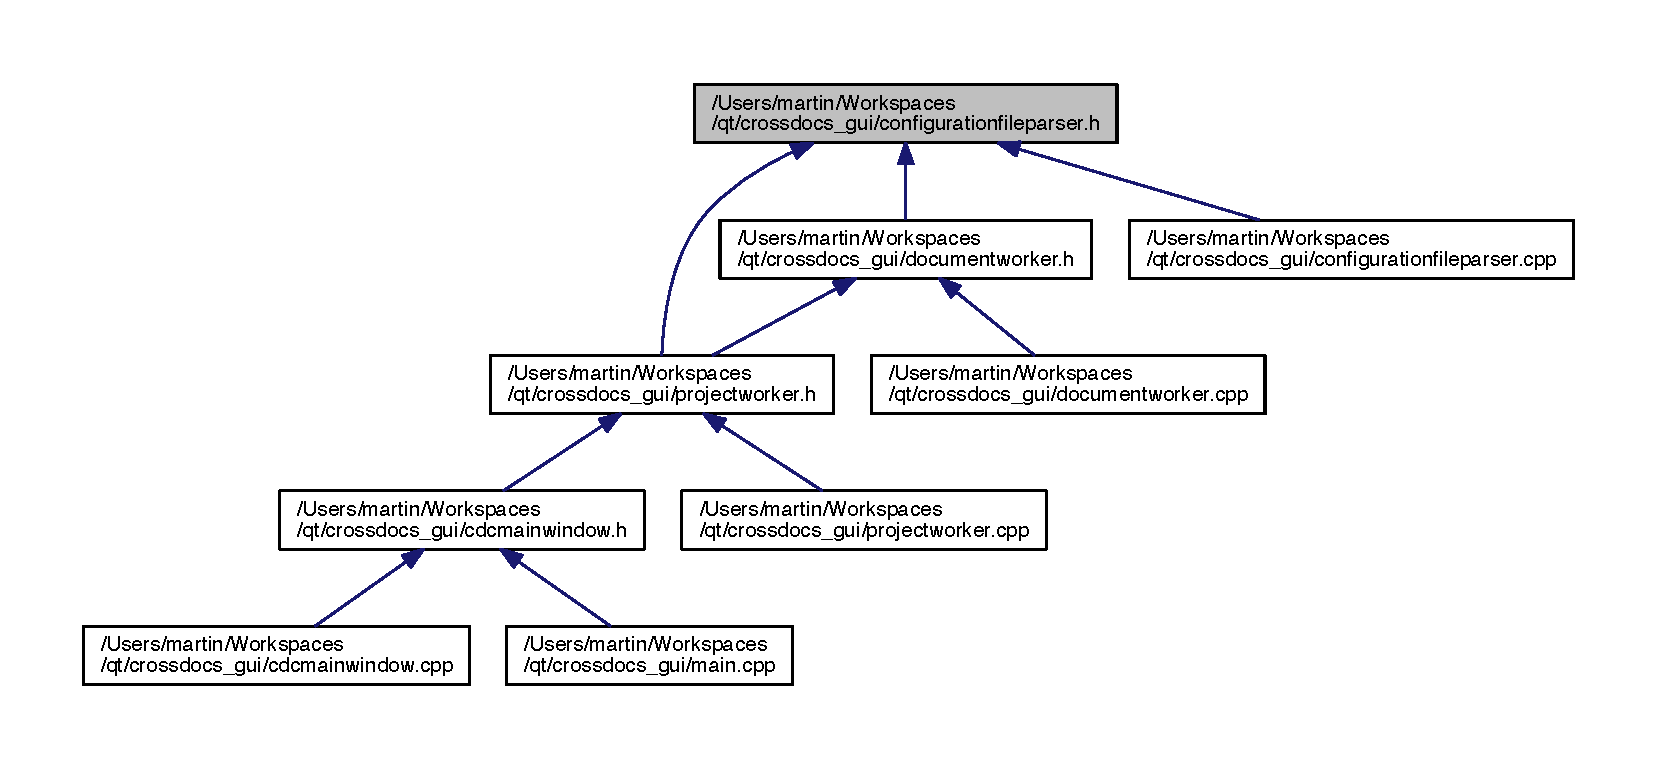
\includegraphics[width=350pt]{configurationfileparser_8h__dep__incl}
\end{center}
\end{figure}
\subsection*{Classes}
\begin{DoxyCompactItemize}
\item 
class \hyperlink{classconfiguration_file_parser}{configuration\+File\+Parser}
\end{DoxyCompactItemize}


\subsection{Detailed Description}
Definitions for $\ast$.cdc file parsing. 



 / \+\_\+\+\_\+ \textbackslash{} $\vert$ \+\_\+ \textbackslash{} $\vert$ / \textbackslash{}/\+\_\+ \+\_\+\+\_\+ \+\_\+\+\_\+\+\_\+ \+\_\+\+\_\+\+\_\+ \+\_\+\+\_\+\+\_\+$\vert$ $\vert$ $\vert$ $\vert$\+\_\+\+\_\+\+\_\+ \+\_\+\+\_\+\+\_\+ \+\_\+\+\_\+\+\_\+ $\vert$ $\vert$ $\vert$ '\+\_\+\+\_\+/ \+\_\+ \textbackslash{}/ \+\_\+\+\_\+/ \+\_\+\+\_\+$\vert$ $\vert$ $\vert$ / \+\_\+ \textbackslash{} / \+\_\+\+\_\+/ \+\_\+\+\_\+$\vert$ $\vert$ \+\_\+\+\_\+/\textbackslash{} $\vert$ $\vert$ $\vert$\+\_\+$\vert$ \+\_\+\+\_\+ \+\_\+\+\_\+ \textbackslash{} $\vert$/ / $\vert$\+\_\+$\vert$ $\vert$ (\+\_\+\+\_\+\+\_\+\+\_\+ \textbackslash{} \+\_\+\+\_\+\+\_\+\+\_\+/\+\_\+$\vert$ \+\_\+\+\_\+\+\_\+/$\vert$\+\_\+\+\_\+\+\_\+/\+\_\+\+\_\+\+\_\+/\+\_\+\+\_\+\+\_\+/ \+\_\+\+\_\+\+\_\+/ \+\_\+\+\_\+\+\_\+$\vert$\+\_\+\+\_\+\+\_\+/

\begin{DoxyAuthor}{Author}
Martin Vincent Bloedorn 
\end{DoxyAuthor}
\begin{DoxyVersion}{Version}
V0.\+1.\+0 
\end{DoxyVersion}
\begin{DoxyDate}{Date}
03-\/\+August-\/2014 
\end{DoxyDate}
\begin{DoxyRefDesc}{Todo}
\item[\hyperlink{todo__todo000002}{Todo}]Add suport for inline comments. \end{DoxyRefDesc}


Definition in file \hyperlink{configurationfileparser_8h_source}{configurationfileparser.\+h}.


\hypertarget{documentworker_8cpp}{\section{/\+Users/martin/\+Workspaces/qt/crossdocs\+\_\+gui/documentworker.cpp File Reference}
\label{documentworker_8cpp}\index{/\+Users/martin/\+Workspaces/qt/crossdocs\+\_\+gui/documentworker.\+cpp@{/\+Users/martin/\+Workspaces/qt/crossdocs\+\_\+gui/documentworker.\+cpp}}
}


C\+D\+C document functions\+: management, build engine, etc.  


{\ttfamily \#include \char`\"{}documentworker.\+h\char`\"{}}\\*
Include dependency graph for documentworker.\+cpp\+:\nopagebreak
\begin{figure}[H]
\begin{center}
\leavevmode
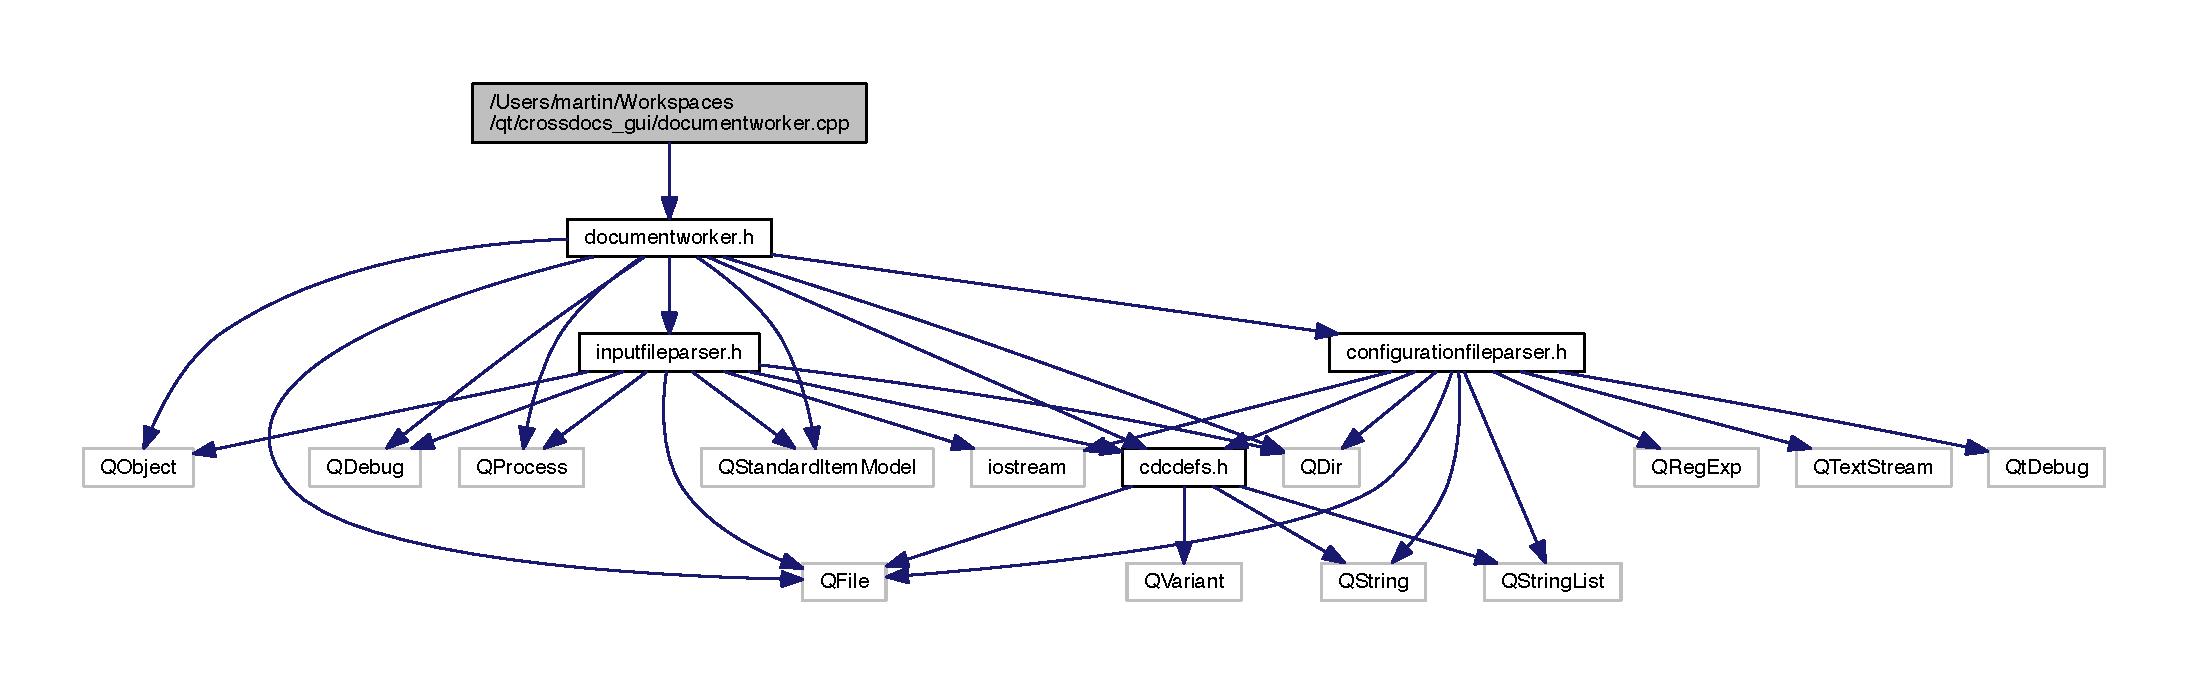
\includegraphics[width=350pt]{documentworker_8cpp__incl}
\end{center}
\end{figure}
\subsection*{Variables}
\begin{DoxyCompactItemize}
\item 
const Q\+String \hyperlink{documentworker_8cpp_afc3552df4a426355881cb35d69445ac0}{docsec\+Tag} = \char`\"{}document\char`\"{}
\item 
const Q\+String \hyperlink{documentworker_8cpp_a3b0ed622aa7a50156b4558bc41361cbb}{docsec\+Name} = \char`\"{}name\char`\"{}
\item 
const Q\+String \hyperlink{documentworker_8cpp_acdacaac08a72e2af86c329afbcff2d99}{docsec\+Input\+Files} = \char`\"{}input\+\_\+files\char`\"{}
\item 
const \hyperlink{cdcdefs_8h_ab649dd84a9663b16384131638df4d313}{C\+D\+C\+\_\+file\+Syntax} \hyperlink{documentworker_8cpp_a2aec0914c76323416c4a6f1a7c6b5c03}{default\+Syntax} = \hyperlink{cdcdefs_8h_abd38cc943467f0d66216a60454d5ee06a1259e5bf3dfd3ef0991fa65ceeda6fec}{C\+D\+C\+\_\+file\+Syntax\+::doxygen}
\end{DoxyCompactItemize}


\subsection{Detailed Description}
C\+D\+C document functions\+: management, build engine, etc. 



 / \+\_\+\+\_\+ \textbackslash{} $\vert$ \+\_\+ \textbackslash{} $\vert$ / \textbackslash{}/\+\_\+ \+\_\+\+\_\+ \+\_\+\+\_\+\+\_\+ \+\_\+\+\_\+\+\_\+ \+\_\+\+\_\+\+\_\+$\vert$ $\vert$ $\vert$ $\vert$\+\_\+\+\_\+\+\_\+ \+\_\+\+\_\+\+\_\+ \+\_\+\+\_\+\+\_\+ $\vert$ $\vert$ $\vert$ '\+\_\+\+\_\+/ \+\_\+ \textbackslash{}/ \+\_\+\+\_\+/ \+\_\+\+\_\+$\vert$ $\vert$ $\vert$ / \+\_\+ \textbackslash{} / \+\_\+\+\_\+/ \+\_\+\+\_\+$\vert$ $\vert$ \+\_\+\+\_\+/\textbackslash{} $\vert$ $\vert$ $\vert$\+\_\+$\vert$ \+\_\+\+\_\+ \+\_\+\+\_\+ \textbackslash{} $\vert$/ / $\vert$\+\_\+$\vert$ $\vert$ (\+\_\+\+\_\+\+\_\+\+\_\+ \textbackslash{} \+\_\+\+\_\+\+\_\+\+\_\+/\+\_\+$\vert$ \+\_\+\+\_\+\+\_\+/$\vert$\+\_\+\+\_\+\+\_\+/\+\_\+\+\_\+\+\_\+/\+\_\+\+\_\+\+\_\+/ \+\_\+\+\_\+\+\_\+/ \+\_\+\+\_\+\+\_\+$\vert$\+\_\+\+\_\+\+\_\+/

\begin{DoxyAuthor}{Author}
Martin Vincent Bloedorn 
\end{DoxyAuthor}
\begin{DoxyVersion}{Version}
V0.\+1.\+0 
\end{DoxyVersion}
\begin{DoxyDate}{Date}
18-\/\+August-\/2014 
\end{DoxyDate}


Definition in file \hyperlink{documentworker_8cpp_source}{documentworker.\+cpp}.



\subsection{Variable Documentation}
\hypertarget{documentworker_8cpp_a2aec0914c76323416c4a6f1a7c6b5c03}{\index{documentworker.\+cpp@{documentworker.\+cpp}!default\+Syntax@{default\+Syntax}}
\index{default\+Syntax@{default\+Syntax}!documentworker.\+cpp@{documentworker.\+cpp}}
\subsubsection[{default\+Syntax}]{\setlength{\rightskip}{0pt plus 5cm}const {\bf C\+D\+C\+\_\+file\+Syntax} default\+Syntax = {\bf C\+D\+C\+\_\+file\+Syntax\+::doxygen}}}\label{documentworker_8cpp_a2aec0914c76323416c4a6f1a7c6b5c03}


Definition at line 25 of file documentworker.\+cpp.

\hypertarget{documentworker_8cpp_acdacaac08a72e2af86c329afbcff2d99}{\index{documentworker.\+cpp@{documentworker.\+cpp}!docsec\+Input\+Files@{docsec\+Input\+Files}}
\index{docsec\+Input\+Files@{docsec\+Input\+Files}!documentworker.\+cpp@{documentworker.\+cpp}}
\subsubsection[{docsec\+Input\+Files}]{\setlength{\rightskip}{0pt plus 5cm}const Q\+String docsec\+Input\+Files = \char`\"{}input\+\_\+files\char`\"{}}}\label{documentworker_8cpp_acdacaac08a72e2af86c329afbcff2d99}


Definition at line 24 of file documentworker.\+cpp.

\hypertarget{documentworker_8cpp_a3b0ed622aa7a50156b4558bc41361cbb}{\index{documentworker.\+cpp@{documentworker.\+cpp}!docsec\+Name@{docsec\+Name}}
\index{docsec\+Name@{docsec\+Name}!documentworker.\+cpp@{documentworker.\+cpp}}
\subsubsection[{docsec\+Name}]{\setlength{\rightskip}{0pt plus 5cm}const Q\+String docsec\+Name = \char`\"{}name\char`\"{}}}\label{documentworker_8cpp_a3b0ed622aa7a50156b4558bc41361cbb}


Definition at line 23 of file documentworker.\+cpp.

\hypertarget{documentworker_8cpp_afc3552df4a426355881cb35d69445ac0}{\index{documentworker.\+cpp@{documentworker.\+cpp}!docsec\+Tag@{docsec\+Tag}}
\index{docsec\+Tag@{docsec\+Tag}!documentworker.\+cpp@{documentworker.\+cpp}}
\subsubsection[{docsec\+Tag}]{\setlength{\rightskip}{0pt plus 5cm}const Q\+String docsec\+Tag = \char`\"{}document\char`\"{}}}\label{documentworker_8cpp_afc3552df4a426355881cb35d69445ac0}


Definition at line 22 of file documentworker.\+cpp.


\hypertarget{documentworker_8h}{\section{/\+Users/martin/\+Workspaces/qt/crossdocs\+\_\+gui/documentworker.h File Reference}
\label{documentworker_8h}\index{/\+Users/martin/\+Workspaces/qt/crossdocs\+\_\+gui/documentworker.\+h@{/\+Users/martin/\+Workspaces/qt/crossdocs\+\_\+gui/documentworker.\+h}}
}
{\ttfamily \#include $<$Q\+Object$>$}\\*
{\ttfamily \#include $<$Q\+Debug$>$}\\*
{\ttfamily \#include $<$Q\+Process$>$}\\*
{\ttfamily \#include $<$Q\+File$>$}\\*
{\ttfamily \#include $<$Q\+Dir$>$}\\*
{\ttfamily \#include $<$Q\+Standard\+Item\+Model$>$}\\*
{\ttfamily \#include \char`\"{}cdcdefs.\+h\char`\"{}}\\*
{\ttfamily \#include \char`\"{}configurationfileparser.\+h\char`\"{}}\\*
{\ttfamily \#include \char`\"{}inputfileparser.\+h\char`\"{}}\\*
Include dependency graph for documentworker.\+h\+:\nopagebreak
\begin{figure}[H]
\begin{center}
\leavevmode
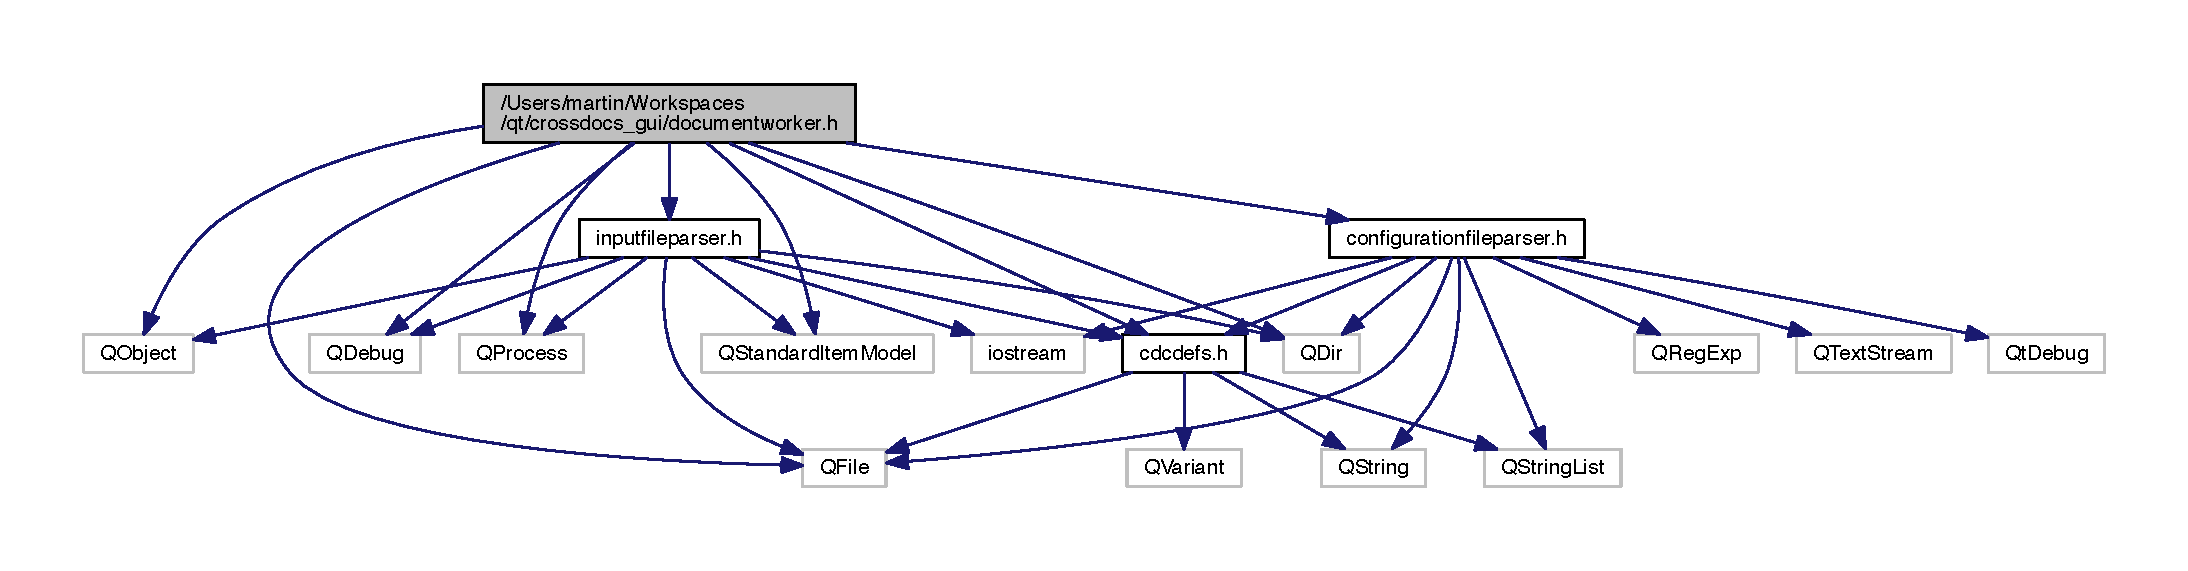
\includegraphics[width=350pt]{documentworker_8h__incl}
\end{center}
\end{figure}
This graph shows which files directly or indirectly include this file\+:\nopagebreak
\begin{figure}[H]
\begin{center}
\leavevmode
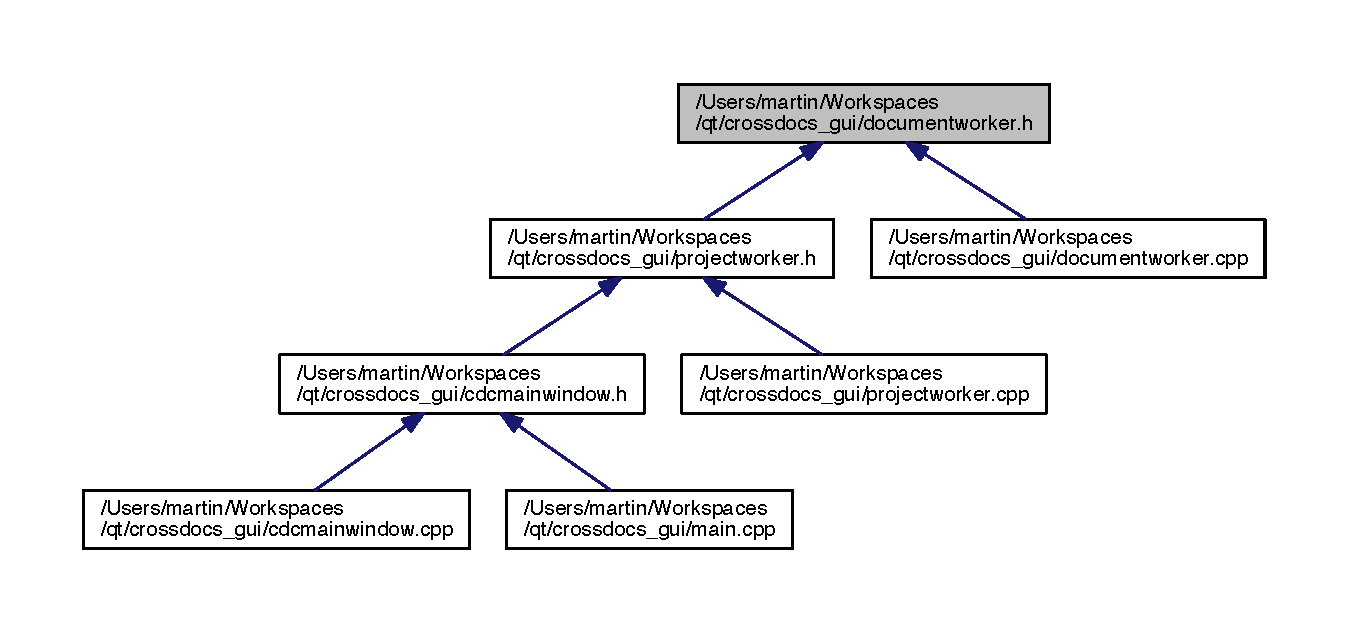
\includegraphics[width=350pt]{documentworker_8h__dep__incl}
\end{center}
\end{figure}
\subsection*{Classes}
\begin{DoxyCompactItemize}
\item 
class \hyperlink{classdocument_worker}{document\+Worker}
\item 
struct \hyperlink{structdocument_worker_1_1_c_d_c__input_file}{document\+Worker\+::\+C\+D\+C\+\_\+input\+File}
\begin{DoxyCompactList}\small\item\em Configuration file for document. \end{DoxyCompactList}\end{DoxyCompactItemize}

\hypertarget{inputfileparser_8cpp}{\section{/\+Users/martin/\+Workspaces/qt/crossdocs\+\_\+gui/inputfileparser.cpp File Reference}
\label{inputfileparser_8cpp}\index{/\+Users/martin/\+Workspaces/qt/crossdocs\+\_\+gui/inputfileparser.\+cpp@{/\+Users/martin/\+Workspaces/qt/crossdocs\+\_\+gui/inputfileparser.\+cpp}}
}


Analyses input file for its sections, subsections, etc.  


{\ttfamily \#include \char`\"{}inputfileparser.\+h\char`\"{}}\\*
Include dependency graph for inputfileparser.\+cpp\+:\nopagebreak
\begin{figure}[H]
\begin{center}
\leavevmode
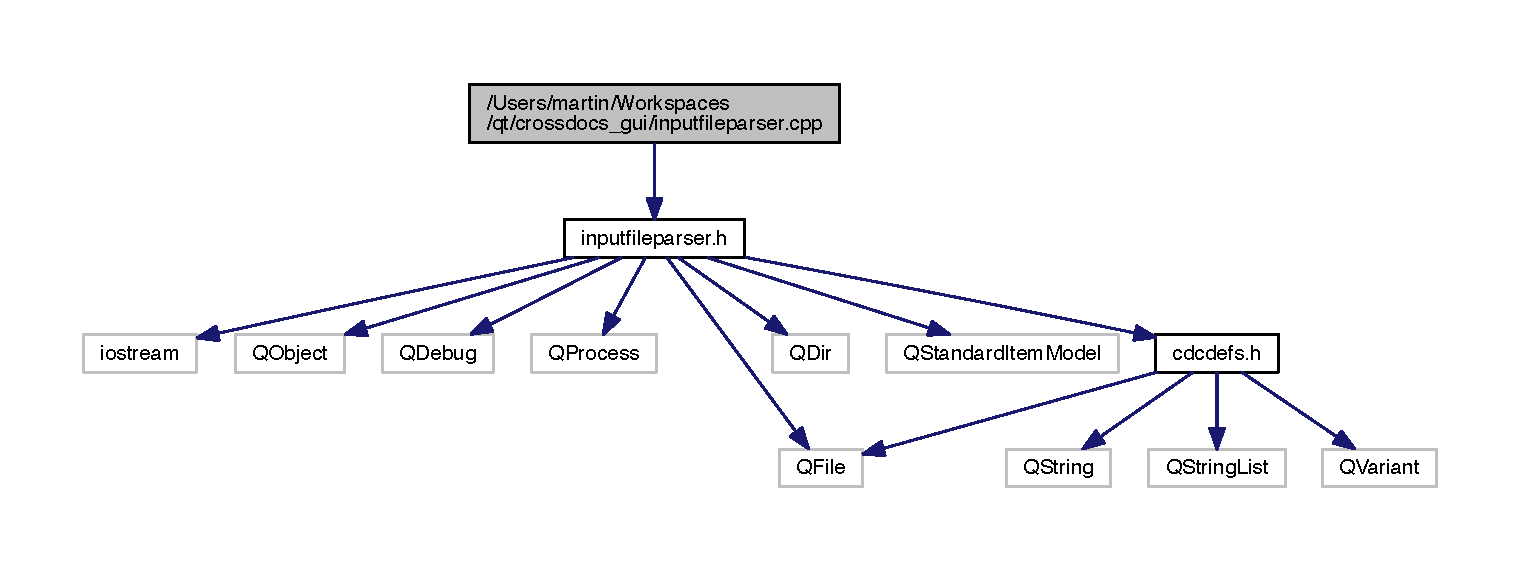
\includegraphics[width=350pt]{inputfileparser_8cpp__incl}
\end{center}
\end{figure}


\subsection{Detailed Description}
Analyses input file for its sections, subsections, etc. 



 / \+\_\+\+\_\+ \textbackslash{} $\vert$ \+\_\+ \textbackslash{} $\vert$ / \textbackslash{}/\+\_\+ \+\_\+\+\_\+ \+\_\+\+\_\+\+\_\+ \+\_\+\+\_\+\+\_\+ \+\_\+\+\_\+\+\_\+$\vert$ $\vert$ $\vert$ $\vert$\+\_\+\+\_\+\+\_\+ \+\_\+\+\_\+\+\_\+ \+\_\+\+\_\+\+\_\+ $\vert$ $\vert$ $\vert$ '\+\_\+\+\_\+/ \+\_\+ \textbackslash{}/ \+\_\+\+\_\+/ \+\_\+\+\_\+$\vert$ $\vert$ $\vert$ / \+\_\+ \textbackslash{} / \+\_\+\+\_\+/ \+\_\+\+\_\+$\vert$ $\vert$ \+\_\+\+\_\+/\textbackslash{} $\vert$ $\vert$ $\vert$\+\_\+$\vert$ \+\_\+\+\_\+ \+\_\+\+\_\+ \textbackslash{} $\vert$/ / $\vert$\+\_\+$\vert$ $\vert$ (\+\_\+\+\_\+\+\_\+\+\_\+ \textbackslash{} \+\_\+\+\_\+\+\_\+\+\_\+/\+\_\+$\vert$ \+\_\+\+\_\+\+\_\+/$\vert$\+\_\+\+\_\+\+\_\+/\+\_\+\+\_\+\+\_\+/\+\_\+\+\_\+\+\_\+/ \+\_\+\+\_\+\+\_\+/ \+\_\+\+\_\+\+\_\+$\vert$\+\_\+\+\_\+\+\_\+/

\begin{DoxyAuthor}{Author}
Martin Vincent Bloedorn 
\end{DoxyAuthor}
\begin{DoxyVersion}{Version}
V0.\+1.\+0 
\end{DoxyVersion}
\begin{DoxyDate}{Date}
24-\/\+August-\/2014 
\end{DoxyDate}


Definition in file \hyperlink{inputfileparser_8cpp_source}{inputfileparser.\+cpp}.


\hypertarget{inputfileparser_8h}{\section{/\+Users/martin/\+Workspaces/qt/crossdocs\+\_\+gui/inputfileparser.h File Reference}
\label{inputfileparser_8h}\index{/\+Users/martin/\+Workspaces/qt/crossdocs\+\_\+gui/inputfileparser.\+h@{/\+Users/martin/\+Workspaces/qt/crossdocs\+\_\+gui/inputfileparser.\+h}}
}
{\ttfamily \#include $<$iostream$>$}\\*
{\ttfamily \#include $<$Q\+Object$>$}\\*
{\ttfamily \#include $<$Q\+Debug$>$}\\*
{\ttfamily \#include $<$Q\+Process$>$}\\*
{\ttfamily \#include $<$Q\+File$>$}\\*
{\ttfamily \#include $<$Q\+Dir$>$}\\*
{\ttfamily \#include $<$Q\+Standard\+Item\+Model$>$}\\*
{\ttfamily \#include \char`\"{}cdcdefs.\+h\char`\"{}}\\*
Include dependency graph for inputfileparser.\+h\+:\nopagebreak
\begin{figure}[H]
\begin{center}
\leavevmode
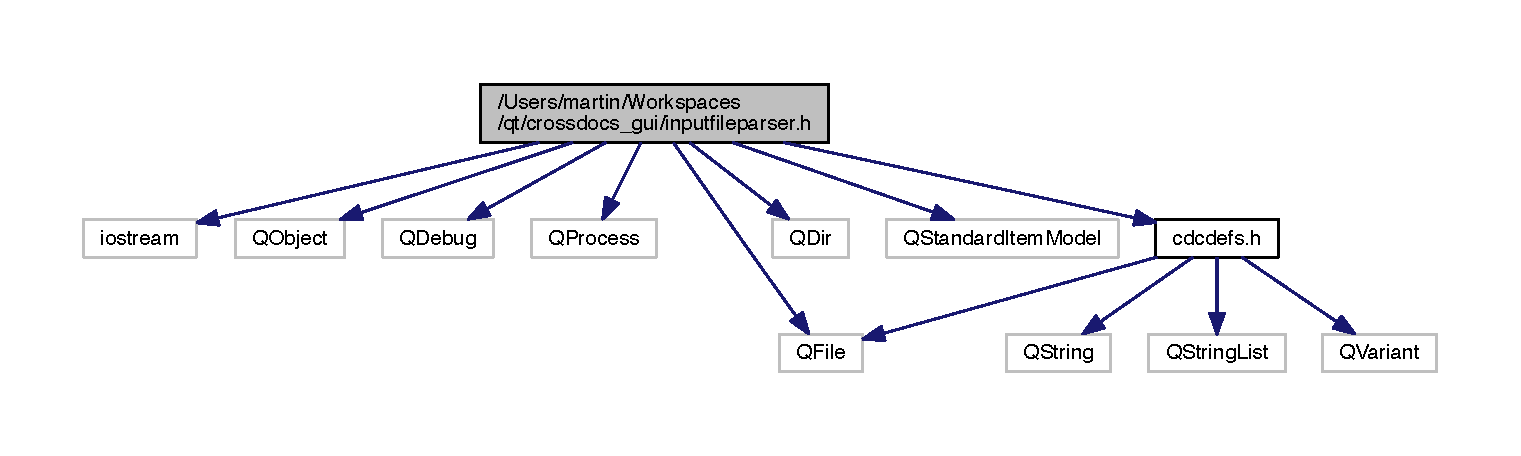
\includegraphics[width=350pt]{inputfileparser_8h__incl}
\end{center}
\end{figure}
This graph shows which files directly or indirectly include this file\+:\nopagebreak
\begin{figure}[H]
\begin{center}
\leavevmode
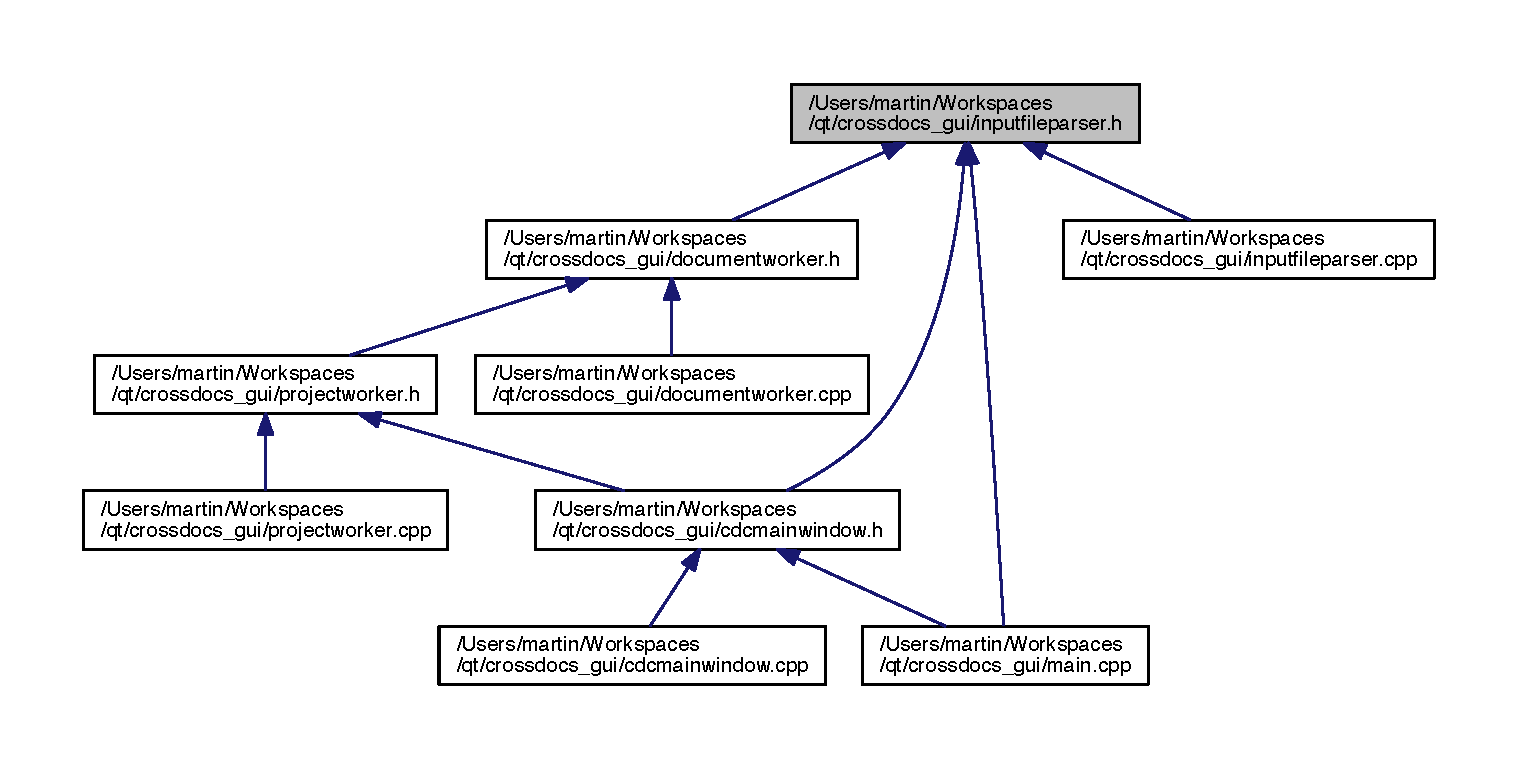
\includegraphics[width=350pt]{inputfileparser_8h__dep__incl}
\end{center}
\end{figure}
\subsection*{Classes}
\begin{DoxyCompactItemize}
\item 
class \hyperlink{classinput_file_parser}{input\+File\+Parser}
\end{DoxyCompactItemize}

\hypertarget{main_8cpp}{\section{/\+Users/martin/\+Workspaces/qt/crossdocs\+\_\+gui/main.cpp File Reference}
\label{main_8cpp}\index{/\+Users/martin/\+Workspaces/qt/crossdocs\+\_\+gui/main.\+cpp@{/\+Users/martin/\+Workspaces/qt/crossdocs\+\_\+gui/main.\+cpp}}
}


Cross\+Docs G\+U\+I entry point.  


{\ttfamily \#include $<$iostream$>$}\\*
{\ttfamily \#include $<$Q\+Debug$>$}\\*
{\ttfamily \#include \char`\"{}cdcmainwindow.\+h\char`\"{}}\\*
{\ttfamily \#include \char`\"{}inputfileparser.\+h\char`\"{}}\\*
Include dependency graph for main.\+cpp\+:\nopagebreak
\begin{figure}[H]
\begin{center}
\leavevmode
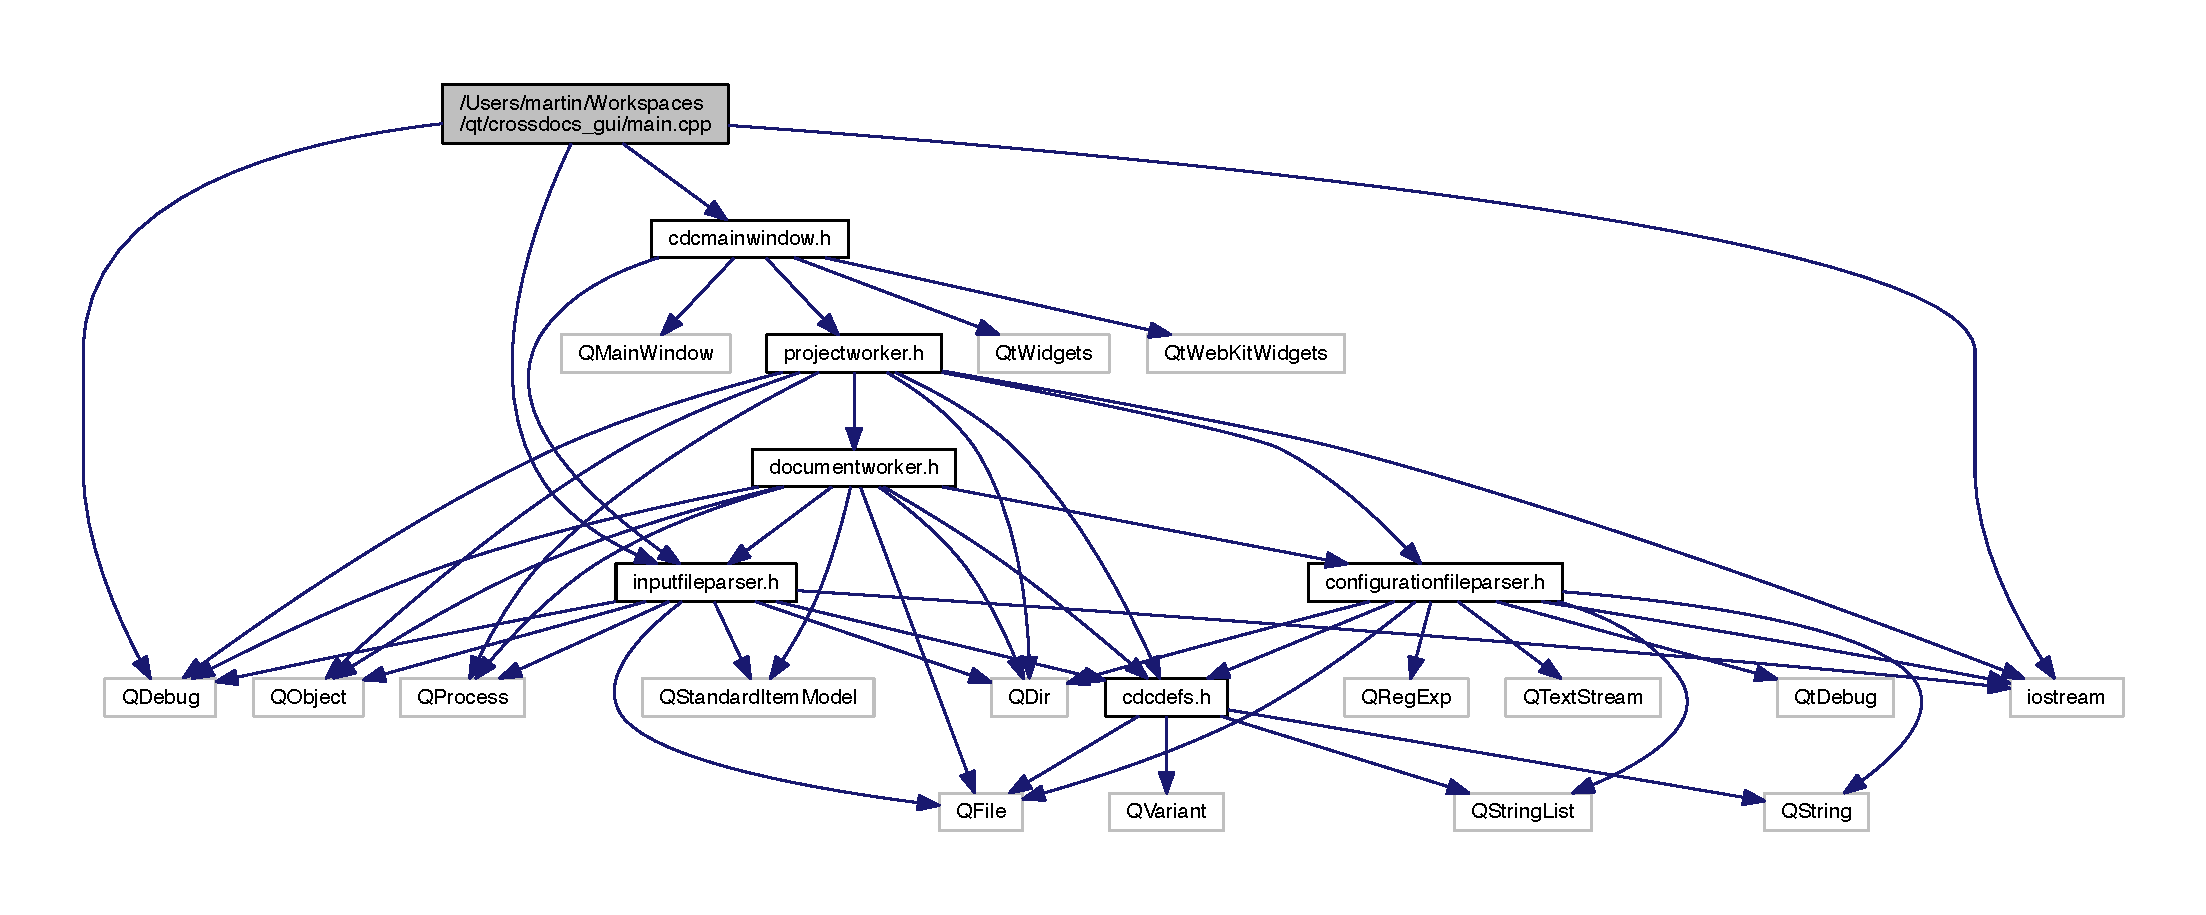
\includegraphics[width=350pt]{main_8cpp__incl}
\end{center}
\end{figure}
\subsection*{Functions}
\begin{DoxyCompactItemize}
\item 
void \hyperlink{main_8cpp_a9606ad1b9a909a366a2d8317438d2e58}{message\+Handler} (Qt\+Msg\+Type type, const Q\+Message\+Log\+Context \&context, const Q\+String \&msg)
\begin{DoxyCompactList}\small\item\em Wrapper for \hyperlink{classcdc_main_window_afe66a2955f78dca82931e14113abd139}{cdc\+Main\+Window\+::message\+Handler} , to use with q\+Install\+Message\+Handler . \end{DoxyCompactList}\item 
int \hyperlink{main_8cpp_a0ddf1224851353fc92bfbff6f499fa97}{main} (int argc, char $\ast$argv\mbox{[}$\,$\mbox{]})
\end{DoxyCompactItemize}
\subsection*{Variables}
\begin{DoxyCompactItemize}
\item 
\hyperlink{classcdc_main_window}{cdc\+Main\+Window} $\ast$ \hyperlink{main_8cpp_a3abf13a47992f76d710377b9d402a52d}{main\+Window}
\end{DoxyCompactItemize}


\subsection{Detailed Description}
Cross\+Docs G\+U\+I entry point. 



 / \+\_\+\+\_\+ \textbackslash{} $\vert$ \+\_\+ \textbackslash{} $\vert$ / \textbackslash{}/\+\_\+ \+\_\+\+\_\+ \+\_\+\+\_\+\+\_\+ \+\_\+\+\_\+\+\_\+ \+\_\+\+\_\+\+\_\+$\vert$ $\vert$ $\vert$ $\vert$\+\_\+\+\_\+\+\_\+ \+\_\+\+\_\+\+\_\+ \+\_\+\+\_\+\+\_\+ $\vert$ $\vert$ $\vert$ '\+\_\+\+\_\+/ \+\_\+ \textbackslash{}/ \+\_\+\+\_\+/ \+\_\+\+\_\+$\vert$ $\vert$ $\vert$ / \+\_\+ \textbackslash{} / \+\_\+\+\_\+/ \+\_\+\+\_\+$\vert$ $\vert$ \+\_\+\+\_\+/\textbackslash{} $\vert$ $\vert$ $\vert$\+\_\+$\vert$ \+\_\+\+\_\+ \+\_\+\+\_\+ \textbackslash{} $\vert$/ / $\vert$\+\_\+$\vert$ $\vert$ (\+\_\+\+\_\+\+\_\+\+\_\+ \textbackslash{} \+\_\+\+\_\+\+\_\+\+\_\+/\+\_\+$\vert$ \+\_\+\+\_\+\+\_\+/$\vert$\+\_\+\+\_\+\+\_\+/\+\_\+\+\_\+\+\_\+/\+\_\+\+\_\+\+\_\+/ \+\_\+\+\_\+\+\_\+/ \+\_\+\+\_\+\+\_\+$\vert$\+\_\+\+\_\+\+\_\+/

\begin{DoxyAuthor}{Author}
Martin Vincent Bloedorn 
\end{DoxyAuthor}
\begin{DoxyVersion}{Version}
V0.\+1.\+0 
\end{DoxyVersion}
\begin{DoxyDate}{Date}
17-\/\+August-\/2014 
\end{DoxyDate}


Definition in file \hyperlink{main_8cpp_source}{main.\+cpp}.



\subsection{Function Documentation}
\hypertarget{main_8cpp_a0ddf1224851353fc92bfbff6f499fa97}{\index{main.\+cpp@{main.\+cpp}!main@{main}}
\index{main@{main}!main.\+cpp@{main.\+cpp}}
\subsubsection[{main}]{\setlength{\rightskip}{0pt plus 5cm}int main (
\begin{DoxyParamCaption}
\item[{int}]{argc, }
\item[{char $\ast$}]{argv\mbox{[}$\,$\mbox{]}}
\end{DoxyParamCaption}
)}}\label{main_8cpp_a0ddf1224851353fc92bfbff6f499fa97}


Definition at line 36 of file main.\+cpp.

\hypertarget{main_8cpp_a9606ad1b9a909a366a2d8317438d2e58}{\index{main.\+cpp@{main.\+cpp}!message\+Handler@{message\+Handler}}
\index{message\+Handler@{message\+Handler}!main.\+cpp@{main.\+cpp}}
\subsubsection[{message\+Handler}]{\setlength{\rightskip}{0pt plus 5cm}void message\+Handler (
\begin{DoxyParamCaption}
\item[{Qt\+Msg\+Type}]{type, }
\item[{const Q\+Message\+Log\+Context \&}]{context, }
\item[{const Q\+String \&}]{msg}
\end{DoxyParamCaption}
)}}\label{main_8cpp_a9606ad1b9a909a366a2d8317438d2e58}


Wrapper for \hyperlink{classcdc_main_window_afe66a2955f78dca82931e14113abd139}{cdc\+Main\+Window\+::message\+Handler} , to use with q\+Install\+Message\+Handler . 



Definition at line 31 of file main.\+cpp.



\subsection{Variable Documentation}
\hypertarget{main_8cpp_a3abf13a47992f76d710377b9d402a52d}{\index{main.\+cpp@{main.\+cpp}!main\+Window@{main\+Window}}
\index{main\+Window@{main\+Window}!main.\+cpp@{main.\+cpp}}
\subsubsection[{main\+Window}]{\setlength{\rightskip}{0pt plus 5cm}{\bf cdc\+Main\+Window}$\ast$ main\+Window}}\label{main_8cpp_a3abf13a47992f76d710377b9d402a52d}


Definition at line 28 of file main.\+cpp.


\hypertarget{projectworker_8cpp}{\section{/\+Users/martin/\+Workspaces/qt/crossdocs\+\_\+gui/projectworker.cpp File Reference}
\label{projectworker_8cpp}\index{/\+Users/martin/\+Workspaces/qt/crossdocs\+\_\+gui/projectworker.\+cpp@{/\+Users/martin/\+Workspaces/qt/crossdocs\+\_\+gui/projectworker.\+cpp}}
}


C\+D\+C document functions\+: management, build engine, etc.  


{\ttfamily \#include \char`\"{}projectworker.\+h\char`\"{}}\\*
Include dependency graph for projectworker.\+cpp\+:\nopagebreak
\begin{figure}[H]
\begin{center}
\leavevmode
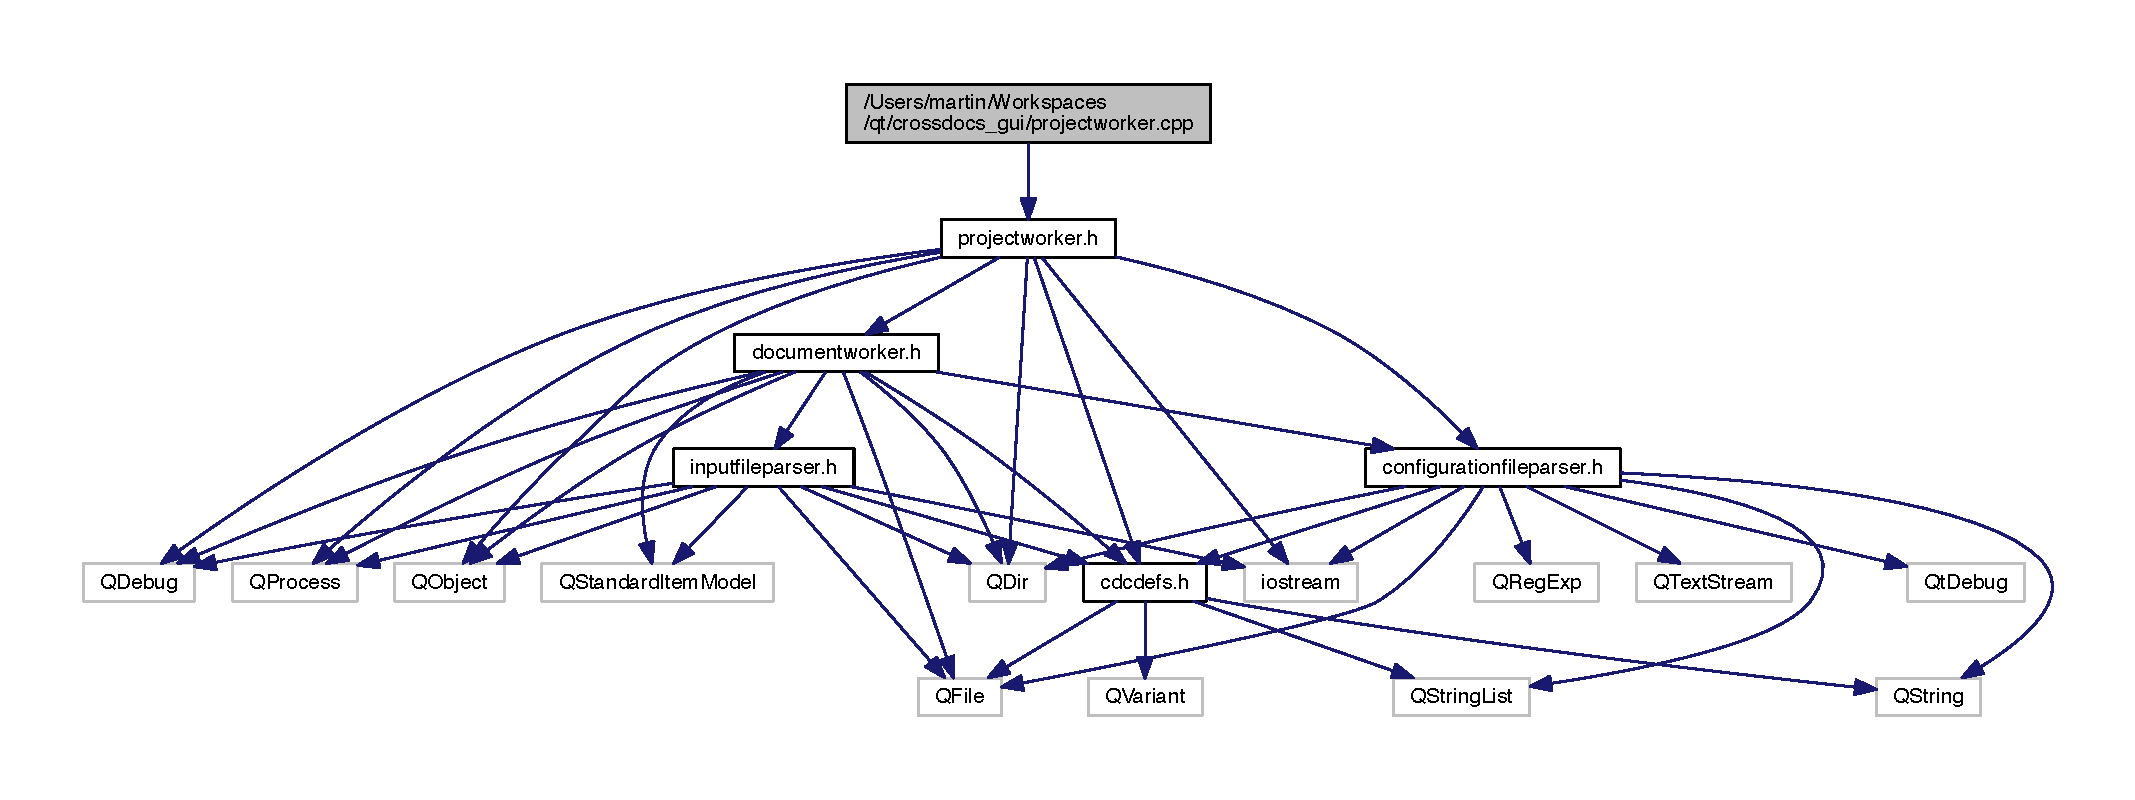
\includegraphics[width=350pt]{projectworker_8cpp__incl}
\end{center}
\end{figure}
\subsection*{Variables}
\begin{DoxyCompactItemize}
\item 
const Q\+String \hyperlink{projectworker_8cpp_a6ab62437500dec27ccbf6c8820ef45ad}{confsec\+Project\+Tag} = \char`\"{}project\char`\"{}
\item 
const Q\+String \hyperlink{projectworker_8cpp_a5aced6af1d7defb36e5083ad4d74f5f5}{confsec\+Documents} = \char`\"{}documents\char`\"{}
\item 
const Q\+String \hyperlink{projectworker_8cpp_a4b48111aab3ea0a416837e8eb0a0caf3}{confsec\+Project\+Name} = \char`\"{}name\char`\"{}
\item 
const Q\+String \hyperlink{projectworker_8cpp_a3ea66eefd25766ac01e25d9c3614f50e}{confsec\+Build\+Engine} = \char`\"{}build\+\_\+engine\char`\"{}
\end{DoxyCompactItemize}


\subsection{Detailed Description}
C\+D\+C document functions\+: management, build engine, etc. 

C\+D\+C project functions\+: management, build engine, etc.



 / \+\_\+\+\_\+ \textbackslash{} $\vert$ \+\_\+ \textbackslash{} $\vert$ / \textbackslash{}/\+\_\+ \+\_\+\+\_\+ \+\_\+\+\_\+\+\_\+ \+\_\+\+\_\+\+\_\+ \+\_\+\+\_\+\+\_\+$\vert$ $\vert$ $\vert$ $\vert$\+\_\+\+\_\+\+\_\+ \+\_\+\+\_\+\+\_\+ \+\_\+\+\_\+\+\_\+ $\vert$ $\vert$ $\vert$ '\+\_\+\+\_\+/ \+\_\+ \textbackslash{}/ \+\_\+\+\_\+/ \+\_\+\+\_\+$\vert$ $\vert$ $\vert$ / \+\_\+ \textbackslash{} / \+\_\+\+\_\+/ \+\_\+\+\_\+$\vert$ $\vert$ \+\_\+\+\_\+/\textbackslash{} $\vert$ $\vert$ $\vert$\+\_\+$\vert$ \+\_\+\+\_\+ \+\_\+\+\_\+ \textbackslash{} $\vert$/ / $\vert$\+\_\+$\vert$ $\vert$ (\+\_\+\+\_\+\+\_\+\+\_\+ \textbackslash{} \+\_\+\+\_\+\+\_\+\+\_\+/\+\_\+$\vert$ \+\_\+\+\_\+\+\_\+/$\vert$\+\_\+\+\_\+\+\_\+/\+\_\+\+\_\+\+\_\+/\+\_\+\+\_\+\+\_\+/ \+\_\+\+\_\+\+\_\+/ \+\_\+\+\_\+\+\_\+$\vert$\+\_\+\+\_\+\+\_\+/

\begin{DoxyAuthor}{Author}
Martin Vincent Bloedorn 
\end{DoxyAuthor}
\begin{DoxyVersion}{Version}
V0.\+1.\+0 
\end{DoxyVersion}
\begin{DoxyDate}{Date}
18-\/\+August-\/2014
\end{DoxyDate}


 / \+\_\+\+\_\+ \textbackslash{} $\vert$ \+\_\+ \textbackslash{} $\vert$ / \textbackslash{}/\+\_\+ \+\_\+\+\_\+ \+\_\+\+\_\+\+\_\+ \+\_\+\+\_\+\+\_\+ \+\_\+\+\_\+\+\_\+$\vert$ $\vert$ $\vert$ $\vert$\+\_\+\+\_\+\+\_\+ \+\_\+\+\_\+\+\_\+ \+\_\+\+\_\+\+\_\+ $\vert$ $\vert$ $\vert$ '\+\_\+\+\_\+/ \+\_\+ \textbackslash{}/ \+\_\+\+\_\+/ \+\_\+\+\_\+$\vert$ $\vert$ $\vert$ / \+\_\+ \textbackslash{} / \+\_\+\+\_\+/ \+\_\+\+\_\+$\vert$ $\vert$ \+\_\+\+\_\+/\textbackslash{} $\vert$ $\vert$ $\vert$\+\_\+$\vert$ \+\_\+\+\_\+ \+\_\+\+\_\+ \textbackslash{} $\vert$/ / $\vert$\+\_\+$\vert$ $\vert$ (\+\_\+\+\_\+\+\_\+\+\_\+ \textbackslash{} \+\_\+\+\_\+\+\_\+\+\_\+/\+\_\+$\vert$ \+\_\+\+\_\+\+\_\+/$\vert$\+\_\+\+\_\+\+\_\+/\+\_\+\+\_\+\+\_\+/\+\_\+\+\_\+\+\_\+/ \+\_\+\+\_\+\+\_\+/ \+\_\+\+\_\+\+\_\+$\vert$\+\_\+\+\_\+\+\_\+/

\begin{DoxyAuthor}{Author}
Martin Vincent Bloedorn 
\end{DoxyAuthor}
\begin{DoxyVersion}{Version}
V0.\+1.\+0 
\end{DoxyVersion}
\begin{DoxyDate}{Date}
17-\/\+August-\/2014 
\end{DoxyDate}


Definition in file \hyperlink{projectworker_8cpp_source}{projectworker.\+cpp}.



\subsection{Variable Documentation}
\hypertarget{projectworker_8cpp_a3ea66eefd25766ac01e25d9c3614f50e}{\index{projectworker.\+cpp@{projectworker.\+cpp}!confsec\+Build\+Engine@{confsec\+Build\+Engine}}
\index{confsec\+Build\+Engine@{confsec\+Build\+Engine}!projectworker.\+cpp@{projectworker.\+cpp}}
\subsubsection[{confsec\+Build\+Engine}]{\setlength{\rightskip}{0pt plus 5cm}const Q\+String confsec\+Build\+Engine = \char`\"{}build\+\_\+engine\char`\"{}}}\label{projectworker_8cpp_a3ea66eefd25766ac01e25d9c3614f50e}


Definition at line 25 of file projectworker.\+cpp.

\hypertarget{projectworker_8cpp_a5aced6af1d7defb36e5083ad4d74f5f5}{\index{projectworker.\+cpp@{projectworker.\+cpp}!confsec\+Documents@{confsec\+Documents}}
\index{confsec\+Documents@{confsec\+Documents}!projectworker.\+cpp@{projectworker.\+cpp}}
\subsubsection[{confsec\+Documents}]{\setlength{\rightskip}{0pt plus 5cm}const Q\+String confsec\+Documents = \char`\"{}documents\char`\"{}}}\label{projectworker_8cpp_a5aced6af1d7defb36e5083ad4d74f5f5}


Definition at line 23 of file projectworker.\+cpp.

\hypertarget{projectworker_8cpp_a4b48111aab3ea0a416837e8eb0a0caf3}{\index{projectworker.\+cpp@{projectworker.\+cpp}!confsec\+Project\+Name@{confsec\+Project\+Name}}
\index{confsec\+Project\+Name@{confsec\+Project\+Name}!projectworker.\+cpp@{projectworker.\+cpp}}
\subsubsection[{confsec\+Project\+Name}]{\setlength{\rightskip}{0pt plus 5cm}const Q\+String confsec\+Project\+Name = \char`\"{}name\char`\"{}}}\label{projectworker_8cpp_a4b48111aab3ea0a416837e8eb0a0caf3}


Definition at line 24 of file projectworker.\+cpp.

\hypertarget{projectworker_8cpp_a6ab62437500dec27ccbf6c8820ef45ad}{\index{projectworker.\+cpp@{projectworker.\+cpp}!confsec\+Project\+Tag@{confsec\+Project\+Tag}}
\index{confsec\+Project\+Tag@{confsec\+Project\+Tag}!projectworker.\+cpp@{projectworker.\+cpp}}
\subsubsection[{confsec\+Project\+Tag}]{\setlength{\rightskip}{0pt plus 5cm}const Q\+String confsec\+Project\+Tag = \char`\"{}project\char`\"{}}}\label{projectworker_8cpp_a6ab62437500dec27ccbf6c8820ef45ad}


Definition at line 22 of file projectworker.\+cpp.


\hypertarget{projectworker_8h}{\section{/\+Users/martin/\+Workspaces/qt/crossdocs\+\_\+gui/projectworker.h File Reference}
\label{projectworker_8h}\index{/\+Users/martin/\+Workspaces/qt/crossdocs\+\_\+gui/projectworker.\+h@{/\+Users/martin/\+Workspaces/qt/crossdocs\+\_\+gui/projectworker.\+h}}
}


C\+D\+C project functions\+: management, build engine, etc.  


{\ttfamily \#include $<$iostream$>$}\\*
{\ttfamily \#include $<$Q\+Object$>$}\\*
{\ttfamily \#include $<$Q\+Debug$>$}\\*
{\ttfamily \#include $<$Q\+Process$>$}\\*
{\ttfamily \#include $<$Q\+Dir$>$}\\*
{\ttfamily \#include \char`\"{}cdcdefs.\+h\char`\"{}}\\*
{\ttfamily \#include \char`\"{}configurationfileparser.\+h\char`\"{}}\\*
{\ttfamily \#include \char`\"{}documentworker.\+h\char`\"{}}\\*
Include dependency graph for projectworker.\+h\+:\nopagebreak
\begin{figure}[H]
\begin{center}
\leavevmode
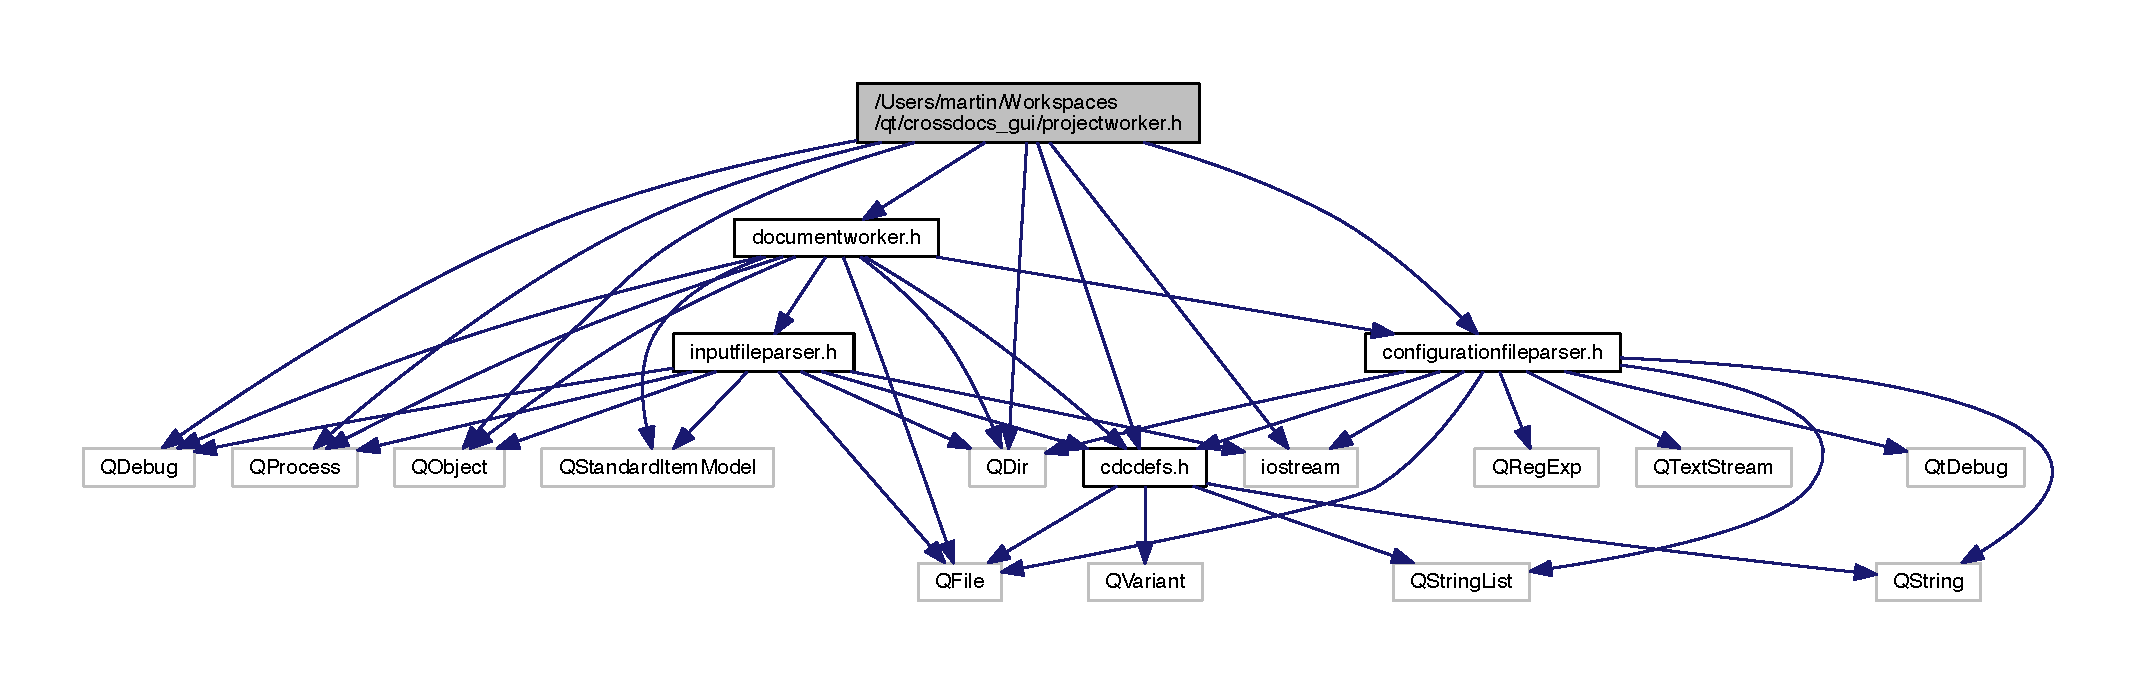
\includegraphics[width=350pt]{projectworker_8h__incl}
\end{center}
\end{figure}
This graph shows which files directly or indirectly include this file\+:\nopagebreak
\begin{figure}[H]
\begin{center}
\leavevmode
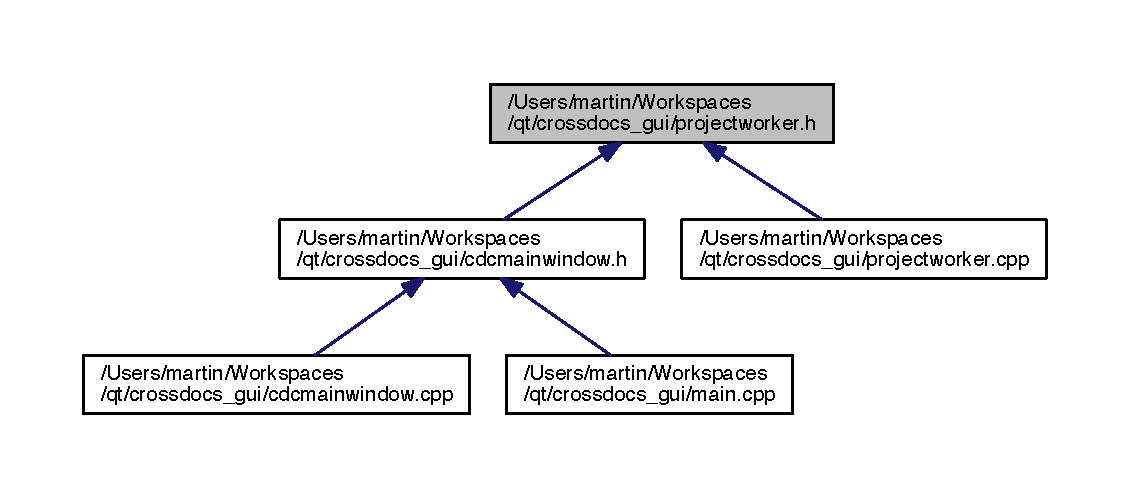
\includegraphics[width=350pt]{projectworker_8h__dep__incl}
\end{center}
\end{figure}
\subsection*{Classes}
\begin{DoxyCompactItemize}
\item 
class \hyperlink{classproject_worker}{project\+Worker}
\end{DoxyCompactItemize}


\subsection{Detailed Description}
C\+D\+C project functions\+: management, build engine, etc. 



 / \+\_\+\+\_\+ \textbackslash{} $\vert$ \+\_\+ \textbackslash{} $\vert$ / \textbackslash{}/\+\_\+ \+\_\+\+\_\+ \+\_\+\+\_\+\+\_\+ \+\_\+\+\_\+\+\_\+ \+\_\+\+\_\+\+\_\+$\vert$ $\vert$ $\vert$ $\vert$\+\_\+\+\_\+\+\_\+ \+\_\+\+\_\+\+\_\+ \+\_\+\+\_\+\+\_\+ $\vert$ $\vert$ $\vert$ '\+\_\+\+\_\+/ \+\_\+ \textbackslash{}/ \+\_\+\+\_\+/ \+\_\+\+\_\+$\vert$ $\vert$ $\vert$ / \+\_\+ \textbackslash{} / \+\_\+\+\_\+/ \+\_\+\+\_\+$\vert$ $\vert$ \+\_\+\+\_\+/\textbackslash{} $\vert$ $\vert$ $\vert$\+\_\+$\vert$ \+\_\+\+\_\+ \+\_\+\+\_\+ \textbackslash{} $\vert$/ / $\vert$\+\_\+$\vert$ $\vert$ (\+\_\+\+\_\+\+\_\+\+\_\+ \textbackslash{} \+\_\+\+\_\+\+\_\+\+\_\+/\+\_\+$\vert$ \+\_\+\+\_\+\+\_\+/$\vert$\+\_\+\+\_\+\+\_\+/\+\_\+\+\_\+\+\_\+/\+\_\+\+\_\+\+\_\+/ \+\_\+\+\_\+\+\_\+/ \+\_\+\+\_\+\+\_\+$\vert$\+\_\+\+\_\+\+\_\+/

\begin{DoxyAuthor}{Author}
Martin Vincent Bloedorn 
\end{DoxyAuthor}
\begin{DoxyVersion}{Version}
V0.\+1.\+0 
\end{DoxyVersion}
\begin{DoxyDate}{Date}
17-\/\+August-\/2014 
\end{DoxyDate}
\begin{DoxyRefDesc}{Todo}
\item[\hyperlink{todo__todo000003}{Todo}]Break front-\/end from back-\/end (C\+L\+I/\+G\+U\+I) 

Add support to create cdd files in non-\/existing folders. \end{DoxyRefDesc}


Definition in file \hyperlink{projectworker_8h_source}{projectworker.\+h}.


\hypertarget{qrc__resources_8cpp}{\section{/\+Users/martin/\+Workspaces/qt/crossdocs\+\_\+gui/qrc\+\_\+resources.cpp File Reference}
\label{qrc__resources_8cpp}\index{/\+Users/martin/\+Workspaces/qt/crossdocs\+\_\+gui/qrc\+\_\+resources.\+cpp@{/\+Users/martin/\+Workspaces/qt/crossdocs\+\_\+gui/qrc\+\_\+resources.\+cpp}}
}
{\ttfamily \#include $<$Qt\+Core/qglobal.\+h$>$}\\*
Include dependency graph for qrc\+\_\+resources.\+cpp\+:\nopagebreak
\begin{figure}[H]
\begin{center}
\leavevmode
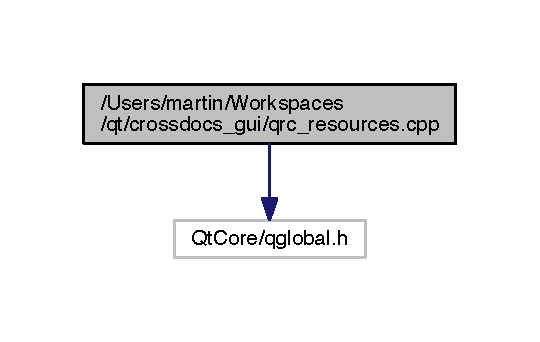
\includegraphics[width=259pt]{qrc__resources_8cpp__incl}
\end{center}
\end{figure}
\subsection*{Functions}
\begin{DoxyCompactItemize}
\item 
Q\+T\+\_\+\+B\+E\+G\+I\+N\+\_\+\+N\+A\+M\+E\+S\+P\+A\+C\+E \\*
Q\+\_\+\+C\+O\+R\+E\+\_\+\+E\+X\+P\+O\+R\+T bool \hyperlink{qrc__resources_8cpp_ab3bec3d1e679084be46edc41e4c91bc1}{q\+Register\+Resource\+Data} (int, const unsigned char $\ast$, const unsigned char $\ast$, const unsigned char $\ast$)
\item 
Q\+\_\+\+C\+O\+R\+E\+\_\+\+E\+X\+P\+O\+R\+T bool \hyperlink{qrc__resources_8cpp_ad65f8bca8010dd1fd135a28a085c6d03}{q\+Unregister\+Resource\+Data} (int, const unsigned char $\ast$, const unsigned char $\ast$, const unsigned char $\ast$)
\item 
Q\+T\+\_\+\+E\+N\+D\+\_\+\+N\+A\+M\+E\+S\+P\+A\+C\+E int \\*
Q\+T\+\_\+\+M\+A\+N\+G\+L\+E\+\_\+\+N\+A\+M\+E\+S\+P\+A\+C\+E() \hyperlink{qrc__resources_8cpp_a9df9503dae688e1ed736f03bf343b6ac}{q\+Init\+Resources\+\_\+resources} ()
\item 
int Q\+T\+\_\+\+M\+A\+N\+G\+L\+E\+\_\+\+N\+A\+M\+E\+S\+P\+A\+C\+E() \hyperlink{qrc__resources_8cpp_aed07cf98f1bcc47e6707bf1b60675291}{q\+Cleanup\+Resources\+\_\+resources} ()
\end{DoxyCompactItemize}


\subsection{Function Documentation}
\hypertarget{qrc__resources_8cpp_aed07cf98f1bcc47e6707bf1b60675291}{\index{qrc\+\_\+resources.\+cpp@{qrc\+\_\+resources.\+cpp}!q\+Cleanup\+Resources\+\_\+resources@{q\+Cleanup\+Resources\+\_\+resources}}
\index{q\+Cleanup\+Resources\+\_\+resources@{q\+Cleanup\+Resources\+\_\+resources}!qrc\+\_\+resources.\+cpp@{qrc\+\_\+resources.\+cpp}}
\subsubsection[{q\+Cleanup\+Resources\+\_\+resources}]{\setlength{\rightskip}{0pt plus 5cm}int Q\+T\+\_\+\+M\+A\+N\+G\+L\+E\+\_\+\+N\+A\+M\+E\+S\+P\+A\+C\+E() q\+Cleanup\+Resources\+\_\+resources (
\begin{DoxyParamCaption}
{}
\end{DoxyParamCaption}
)}}\label{qrc__resources_8cpp_aed07cf98f1bcc47e6707bf1b60675291}


Definition at line 29781 of file qrc\+\_\+resources.\+cpp.

\hypertarget{qrc__resources_8cpp_a9df9503dae688e1ed736f03bf343b6ac}{\index{qrc\+\_\+resources.\+cpp@{qrc\+\_\+resources.\+cpp}!q\+Init\+Resources\+\_\+resources@{q\+Init\+Resources\+\_\+resources}}
\index{q\+Init\+Resources\+\_\+resources@{q\+Init\+Resources\+\_\+resources}!qrc\+\_\+resources.\+cpp@{qrc\+\_\+resources.\+cpp}}
\subsubsection[{q\+Init\+Resources\+\_\+resources}]{\setlength{\rightskip}{0pt plus 5cm}Q\+T\+\_\+\+E\+N\+D\+\_\+\+N\+A\+M\+E\+S\+P\+A\+C\+E int Q\+T\+\_\+\+M\+A\+N\+G\+L\+E\+\_\+\+N\+A\+M\+E\+S\+P\+A\+C\+E() q\+Init\+Resources\+\_\+resources (
\begin{DoxyParamCaption}
{}
\end{DoxyParamCaption}
)}}\label{qrc__resources_8cpp_a9df9503dae688e1ed736f03bf343b6ac}


Definition at line 29772 of file qrc\+\_\+resources.\+cpp.

\hypertarget{qrc__resources_8cpp_ab3bec3d1e679084be46edc41e4c91bc1}{\index{qrc\+\_\+resources.\+cpp@{qrc\+\_\+resources.\+cpp}!q\+Register\+Resource\+Data@{q\+Register\+Resource\+Data}}
\index{q\+Register\+Resource\+Data@{q\+Register\+Resource\+Data}!qrc\+\_\+resources.\+cpp@{qrc\+\_\+resources.\+cpp}}
\subsubsection[{q\+Register\+Resource\+Data}]{\setlength{\rightskip}{0pt plus 5cm}Q\+T\+\_\+\+B\+E\+G\+I\+N\+\_\+\+N\+A\+M\+E\+S\+P\+A\+C\+E Q\+\_\+\+C\+O\+R\+E\+\_\+\+E\+X\+P\+O\+R\+T bool q\+Register\+Resource\+Data (
\begin{DoxyParamCaption}
\item[{int}]{, }
\item[{const unsigned char $\ast$}]{, }
\item[{const unsigned char $\ast$}]{, }
\item[{const unsigned char $\ast$}]{}
\end{DoxyParamCaption}
)}}\label{qrc__resources_8cpp_ab3bec3d1e679084be46edc41e4c91bc1}
\hypertarget{qrc__resources_8cpp_ad65f8bca8010dd1fd135a28a085c6d03}{\index{qrc\+\_\+resources.\+cpp@{qrc\+\_\+resources.\+cpp}!q\+Unregister\+Resource\+Data@{q\+Unregister\+Resource\+Data}}
\index{q\+Unregister\+Resource\+Data@{q\+Unregister\+Resource\+Data}!qrc\+\_\+resources.\+cpp@{qrc\+\_\+resources.\+cpp}}
\subsubsection[{q\+Unregister\+Resource\+Data}]{\setlength{\rightskip}{0pt plus 5cm}Q\+\_\+\+C\+O\+R\+E\+\_\+\+E\+X\+P\+O\+R\+T bool q\+Unregister\+Resource\+Data (
\begin{DoxyParamCaption}
\item[{int}]{, }
\item[{const unsigned char $\ast$}]{, }
\item[{const unsigned char $\ast$}]{, }
\item[{const unsigned char $\ast$}]{}
\end{DoxyParamCaption}
)}}\label{qrc__resources_8cpp_ad65f8bca8010dd1fd135a28a085c6d03}

%--- End generated contents ---

% Index
\newpage
\phantomsection
\addcontentsline{toc}{chapter}{Index}
\printindex

\end{document}
